\documentclass[10pt,doc,floatsintext,apacite]{apa6}
%\documentclass[10pt,journal,compsoc]{IEEEtran}
%\smartqed
\setcounter{secnumdepth}{2}
\usepackage[justification=centering]{caption}
\captionsetup{font={scriptsize}}
\usepackage[ruled]{algorithm2e}
\usepackage{algorithmic}
% \usepackage{times,amsmath,epsfig,proof,url}
\usepackage{amsmath}
\usepackage{indentfirst}
\usepackage{epsfig}
\usepackage{ulem}
% \usepackage{epstopdf}
\usepackage{listings}
\usepackage{subfig}
\usepackage{lipsum}
% \usepackage{subfigure}
%\usepackage{algorithmic}
% \usepackage{multicol,multirow}
% \usepackage{algorithm}
% \usepackage[noend]{algpseudocode}
% \usepackage{textcomp}
\usepackage{color}
%\usepackage[lined,algonl,ruled]{algorithm2e}
% \usepackage{subfigure}
\usepackage{graphicx}
\usepackage[T1]{fontenc}
\newcommand{\secref}[1]{Section \ref{#1}}
\newcommand{\figref}[1]{Figure \ref{#1}}
\newcommand{\tabref}[1]{Table \ref{#1}}
\newcommand{\equref}[1]{Equation (\ref{#1})}
\renewcommand{\algorithmicrequire}{\textbf{Input:}}
\renewcommand{\algorithmicensure}{\textbf{Output:}}
\newcommand{\KZ}[1]{\textcolor{red}{[Kenny: #1]}}
%\newcommand{\JY}[1]{\textcolor{blue}{[Jinyi: #1]}}
\newcommand{\KQ}[1]{\textcolor{red}{[#1]}}
\lstset{
  captionpos=b,
  tabsize=2,
  % numbers=left,
  % numberstyle=\tiny,
  % numbersep=5pt,
  breaklines=true,
  showstringspaces=true,
  basicstyle=\small,
  frame=none,
  emph={label},
  escapechar=* % Escape to LaTeX between |...|
}

\renewcommand{\algorithmcfname}{ALGORITHM}
\SetAlFnt{\small}
\SetAlCapFnt{\small}
\SetAlCapNameFnt{\small}
%\SetAlCapHSkip{0pt}
%\IncMargin{-\parindent}
%\title{Fault-tolerant Information Extraction from OCR Medical Images}
\title{
%Parsing Text in Medical Images via a Space-aware Data Description Language
Layout-aware Information Extraction from Semi-structured Medical Images
}
\shorttitle{Luo et al.}

\twoauthors{Kangqi Luo, Jinyi Lu, Kenny Q. Zhu}{Weiguo Gao, Jia Wei, Meizhuo Zhang}
%\twoaffiliations{Institute of Psychology}{Freud's Institute}

\twoaffiliations{Shanghai Jiao Tong University}{AstraZeneca China}
\abstract{
Digitizing paper documents and extracting structured information is an
important part of information retrieval and knowledge discovery.
Optical character recognition (OCR) has been widely used
in this task, and achieved promising results on textual documents
%and promising results have been achieved in applying OCR to textual documents,
such as books and reports.
For %semi-structured
medical images that combine graphics and words,
%extraction of useful textual information is difficult
due to the discontinuity of text flows,
extracting structured data from them becomes more challenging.
In this paper, we propose a
domain-specific language, called ODL, which allows users to describe
the value and layout format of text data contained in the images.
Based on the value and spatial constraints described in ODL,
the ODL parser parses the raw OCR output XML into a parse tree,
associating values found in the image with the data structure in the
ODL description, while conforming to the aforementioned constraints.
Robustness is the major advantage during this parsing process,
as the parser doesn't rely on carefully annotated bounding boxes
of structured data in the medical image,
and is able to tolerate or even automatically correct some of the errors
introduced by OCR.
% Moreover, the system guides the user in determining where to make incremental corrections to
% the parsing results and learns from these corrections to make better parses in the future.
Compared with baseline methods in the same task,
our ODL parser shows the better tolerance of positional variances between
images, and consistently outperforms existing approaches in terms of
extraction accuracy. This accuracy can be further improved by
learning from a few manual corrections.
}
%\rightheader{Fault-tolerant Information Extraction from OCR Medical Images}
%\leftheader{Jinyi et al.}
\begin{document}
%\small
% \markboth{IEEE TRANSACTIONS ON KNOWLEDGE AND DATA ENGINEERING}{Lu \textit{et al.}: Fault-Tolerant Optical Character Recognition from Semi-structured Medical Images}
% \markboth{L}{R}
%\markboth{Lu \textit{et al.}{Fault-Tolerant Optical Character Recognition from %Semi-structured Medical Images}
%\markboth{Lu et al.}{Fault-Tolerant Optical Character Recognition from Semi-structured Medical Images}

% Fault-tolerant Optical Character Recognition
% from Semi-structured Medical Images

% \author
% {Jinyi Lu{\small $^{1}$}, Kenny Q. Zhu{\small $^{2}$},
% Weiguo Gao{\small $^{3}$}, Jia Wei{\small $^{4}$}
% and Meizhuo Zhang{\small $^{5}$}
% \vspace{1.6mm}\\
% \fontsize{10}{10}\selectfont\itshape
% $^{1,2}$ Shanghai Jiao Tong University\\
% $^{3,4,5}$ AstraZeneca China
% \vspace{1.6mm}\\
% \fontsize{9}{9}\selectfont\ttfamily\upshape
% $^{1}$jinyilu93@gmail.com,
% $^{2}$kzhu@cs.sjtu.edu.cn\\
% $^{3,4,5}$\{Weiguo.Gao,Jenny.Wei,Meizhuo.Zhang\}@astrazeneca.com
% \thanks{Kenny Q. Zhu and Jia Wei are the corresponding authors.}}


%\institute{Jinyi Lu \at
%              Shanghai Jiao Tong University \\
%			  \email{JinyiLu93@egmail.com}           %  \\
%%             \emph{Present address:} of F. Author  %  if needed
%           \and
%           Jialing Pei \at
%              Shanghhai Jiao Tong University \\
%              \email{peijialing@sjtu.edu.cn}
%            \and
%            Kenny Q. Zhu \at
%              Shanghai Jiao Tong University\\
%              \email{kzhu@cs.sjtu.edu.cn}
%            \and
%            Weiguo Gao \at
%              AstraZeneca China\\
%              \email{Weiguo.Gao@astrazeneca.com}
%            \and
%            Jia Wei \at
%              AstraZeneca China\\
%              \email{Jenny.Wei@astrazeneca.com}
%            \and
%            Meizhuo Zhang \at
%              AstraZeneca China\\
%              \email{Meizhuo.Zhang@astrazeneca.com}
%}
%\IEEEtitleabstractindextext{%
%\begin{abstract}
%\end{abstract}

% Note that keywords are not normally used for peerreview papers.
%\begin{IEEEkeywords}
%Information extraction, optical character recognition, document analysis,
%specialized application languages, fuzzy parser, spatial information,
%medical images, medical information systems
%\end{IEEEkeywords}}
\keywords{information extraction,
domain-specific language,
spatial information,
medical images,
optical character recognition,
document analysis}
%specialized application languages,
%fuzzy parser,
%medical information systems


% Multifrequency media access control has been well understood in
% general wireless ad hoc networks, while in wireless sensor networks,
% researchers still focus on single frequency solutions. In wireless
% sensor networks, each device is typically equipped with a single
% radio transceiver and applications adopt much smaller packet sizes
% compared to those in general wireless ad hoc networks. Hence, the
% multifrequency MAC protocols proposed for general wireless ad hoc
% networks are not suitable for wireless sensor network applications,
% which we further demonstrate through our simulation experiments. In
% this article, we propose MMSN, which takes advantage of
% multifrequency availability while, at the same time, takes into
% consideration the restrictions of wireless sensor networks. Through
% extensive experiments, MMSN exhibits the prominent ability to utilize
% parallel transmissions among neighboring nodes. When multiple physical
% frequencies are available, it also achieves increased energy
% efficiency, demonstrating the ability to work against radio
% interference and the tolerance to a wide range of measured time
% synchronization errors.
%\keywords
%{Information extraction, optical character recognition, document analysis,
%specialized application languages, fuzzy parser, spatial information,
%medical images, medical information systems}

\maketitle

%\author{Jinyi Lu, Jialing Pei, Kenny Q. Zhu,
%Weiguo Gao, Jia Wei and Meizhuo Zhang%
%\thanks{J. Lu, J. Pei and K. Q. Zhu are with the Department of Computer Science, Shanghai Jiao Tong University, 800 Dongchuan Road, Shanghai 200240, P.R. China.
%E-mail: JinyiLu93@gmail.com, peijialing@sjtu.edu.cn, kzhu@cs.sjtu.edu.cn.}
%\thanks{W. Gao, J. Wei and M. Zhang are with AstraZeneca China,
%199 Liangjing Road, Shanghai 201203, P.R. China.
%E-mail:Weiguo.Gao@astrazeneca.com, Jenny.Wei@astrazeneca.com, Meizhuo.Zhang@astrazeneca.com.}
% \IEEEcompsocitemizethanks{\IEEEcompsocthanksitem
% J. Lu and K. Q. Zhu are with the Department of Computer Science, Shanghai Jiao Tong University, 800 Dongchuan Road, Shanghai 200240, P.R. China. \protect\\
% E-mail: JinyiLu93@gmail.com, kzhu@cs.sjtu.edu.cn.
% \IEEEcompsocthanksitem W. Gao, J. Wei and M. Zhang are with AstraZeneca China,
% 199 Liangjing Road, Shanghai 201203, P.R. China. \protect\\
% E-mail:\{Weiguo.Gao, Jenny.Wei, Meizhuo.Zhang\}@astrazeneca.com.}% <-this % stops an unwanted space
% \thanks{K. Q. Zhu and J. Wei are the corresponding authors.}
%



% J. Doe and J. Doe are with Anonymous University.}% <-this % stops an unwanted space
% \thanks{Manuscript received April 19, 2005; revised September 17, 2014.}}

% \author{Michael~Shell,~\IEEEmembership{Member,~IEEE,}
%         John~Doe,~\IEEEmembership{Fellow,~OSA,}
%         and~Jane~Doe,~\IEEEmembership{Life~Fellow,~IEEE}% <-this % stops a space
% \IEEEcompsocitemizethanks{\IEEEcompsocthanksitem M. Shell is with the Department
% of Electrical and Computer Engineering, Georgia Institute of Technology, Atlanta,
% GA, 30332.\protect\\
% % note need leading \protect in front of \\ to get a newline within \thanks as
% % \\ is fragile and will error, could use \hfil\break instead.
% E-mail: see http://www.michaelshell.org/contact.html
% \IEEEcompsocthanksitem J. Doe and J. Doe are with Anonymous University.}% <-this % stops an unwanted space
% \thanks{Manuscript received April 19, 2005; revised September 17, 2014.}}
% \pagestyle{myheadings}
% \markboth{IEEE TRANSACTIONS ON PATTERN ANALYSIS AND MACHINE INTELLIGENCE}{Jinyi \MakeLowercase{\textit{et al.}}: Fault-Tolerant Optical Character Recognition from Semi-structured Medical Images}

% \IEEEtitleabstractindextext{%


% Note that keywords are not normally used for peerreview papers.


% }


%\begin{bottomstuff}
%	J. Lu, J. Pei and K. Q. Zhu are with the Department of Computer Science, Shanghai Jiao Tong University, 800 Dongchuan Road, Shanghai 200240, P.R. China.
%	E-mail: JinyiLu93@gmail.com, peijialing@sjtu.edu.cn, kzhu@cs.sjtu.edu.cn.
%	W. Gao, J. Wei and M. Zhang are with AstraZeneca China,
%	199 Liangjing Road, Shanghai 201203, P.R. China.
%	E-mail:Weiguo.Gao@astrazeneca.com, Jenny.Wei@astrazeneca.com, Meizhuo.Zhang@astrazeneca.com.
%\end{bottomstuff}

%\IEEEdisplaynontitleabstractindextext
%\IEEEpeerreviewmaketitle

% \section{Introduction}

Protein$-$protein interactions (PPIs) are of central importance for the majority of biological functions, such as signal transduction, metabolic pathways, molecular dynamics, and protein networks\cite{Hoffmann.Krallinger.ea:2005}, for they serve as the most fundamental building blocks of the entire interacademic systems of any organisms. Collecting data on pairwise interaction relationships is essential for multiple purpose, including identification of modules with certain functionality\cite{Spirin.Mirny.03}, mapping diseases to dominated genes\cite{Ideker.Sharan.08}, and after all, understanding wholistic metabolic/genetic networks from a system biology perspective.

A lot of databases have been built to store protein and genetic interactions from major model organism species and are available in various standardized formats, such as MINT\cite{Zanzoni.Montecchi-Palazzi.ea:2002}, BIND\cite{Bader.ea:2003}, BIOGRID\cite{DBLP:journals/nar/StarkBRBBT06}, etc. Among those mainstream databases, the data largely rely on voluntary reports by scientists or researchers, besides, comprehensive curation efforts become indispensable for the sake of accuracy. However, the amount of biology-related literatures with respect to protein interactions grows explosively and thus make it either impossible or impractical to manually detect PPI information anymore.

Considering huge amount of PPI information with great wealth hidden in published papers, in recent years, numerous mining techniques have been proposed that aim to extract PPI information automatically from free text, especially machine learning, information retrieval, and natural language processing\cite{DBLP:journals/bib/WinnenburgWPDS08}.These approaches can be roughly categorized into three classes: co$-$occurrence, rule$-$based, and machine learning. 

Co$-$occurrence is the approach with most simplicity and naivete. Just as its name implies, this method intends to find out pairs of proteins that co-occur in the same context. The scope of "same context" ranges from phrase, sentence, paragraph to whole abstract, even document. The underlying assumption is that whenever two proteins are mentioned together by authors, chances are high that there is some kind of relationship between them. However, however, in-context closeness even semantic relation does not necessarily represent actual biological interaction. As a consequence, a large fraction of candidate pairs are mismatched inevitably, causing a high recall but low precision.

The second approach is rule-based extraction, in other words, pattern matching. There are many types of rules, most of them concern natural language processing (NLP). One way is to specify hand-crafted regular expressions before hand, which mostly lean on language usage preference. Besides, by using full or partial (shallow) parsing strategies, more information would be acquired, such as part-of-speech taggers, local dependencies between syntactic components, context-free grammar\cite{DBLP:journals/bioinformatics/TemkinG03}, and full sentence structure. Compared to co$-$occurrence, rule-based approach enjoy better precision but much lower recall. In addition, since the rules are usually derived from training data, that is to say, the improper choice of training data would be significantly lethal, therefore quality of extraction is invariably instable and may not applicable to other data.

The third and most commonly used approach use machine learning techniques, in this case, the task to extract protein$-$protein interactions turns out to be a binary classification problem. Each protein pairs are represented along with a set of features, which is associated with their context, then a well$-$defined classifier gives the answer whether the candidate protein pairs is classified to be qualified PPI. (TO BE FURTHER FILLED!!!)

In this paper, we introduce a general bootstrapping framework for Protein$-$protein interaction extraction from natural text.Our method differs from most of the previous works in three aspects:

(1)The extraction process is driven by only tiny fraction of training data, which are regarded as seed data. In each round, it would derive reliable patterns automatically from seed data, then extract more positive PPI pairs consequently, what's more, the seed data would be augmented by the newly extracted results with high confidence.

(2)multiple graph kernel. 

(3)various evaluation.




\section{Introduction}
\label{sec:intro}

% Part 1: Text IE, scenarios, OCR
% What is text information extraction?
Information extraction is the task of automatically extracting information
or knowledge from unstructured or semi-structured documents.
In the domain of image processing,
the task of textual information extraction (TIE)
is automatically detecting and recognizing texts from given images.
% where is it used?
TIE is applied in a large variety of image categories,
such as printed books, newspapers, digital drawings,
or even more general images~\cite{jung2004text}.
% What's the kernel technique?
Optical character recognition (OCR) is the popular approach to solve TIE,
turning images of printed text into machine encoded texts.
OCR is a hot research topic in recent years, and the performance is promising
on \st{plain-text-based images} \KQ{images containing largely text},
such as novels and reports.
For example, Tesseract~\cite{smith2007overview},
one of the most popular open source multilingual recognizers,
achieved an error rate of 3.72\% for recognizing English words
and 3.77\% for simplified Chinese characters\cite{smith2009adapting}.
Based on the exclusive use and high accuracy of OCR,
the Google Books~\cite{vincent2007google} and Gutenberg Project~\cite{lebert2008project}
have scanned a large number of printed books
and converted into text for free and open access.

\begin{figure*}[!htb]
\centering
\subfloat[ECG]{
\label{fig:medicalimage:ecg}
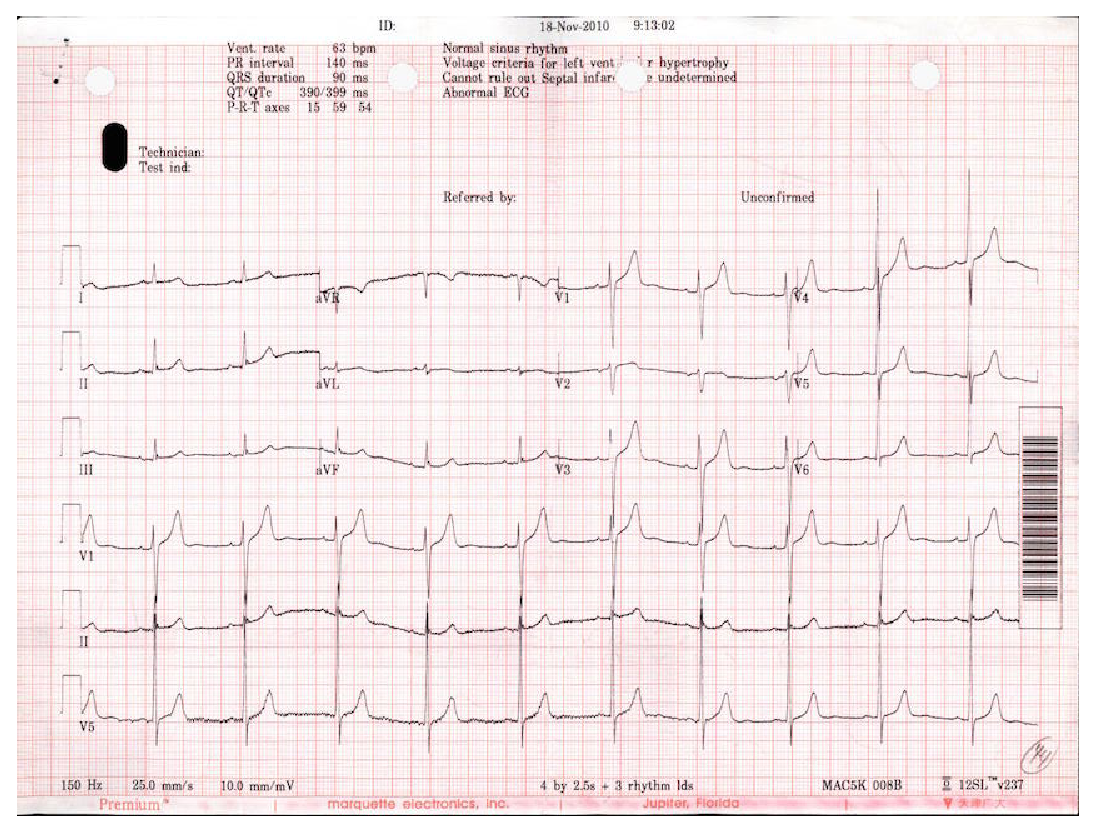
\epsfig{file=figure/ECG.eps, width=1.10\columnwidth}
}
% % \hfill
% \subfloat[X-RAY]{
% \label{fig:medicalimage:xray}
% \epsfig{file=figure/X-RAY.eps, width=0.4\columnwidth}
% }
% \hfill
\subfloat[MRI]{
\label{fig:medicalimage:mrt}
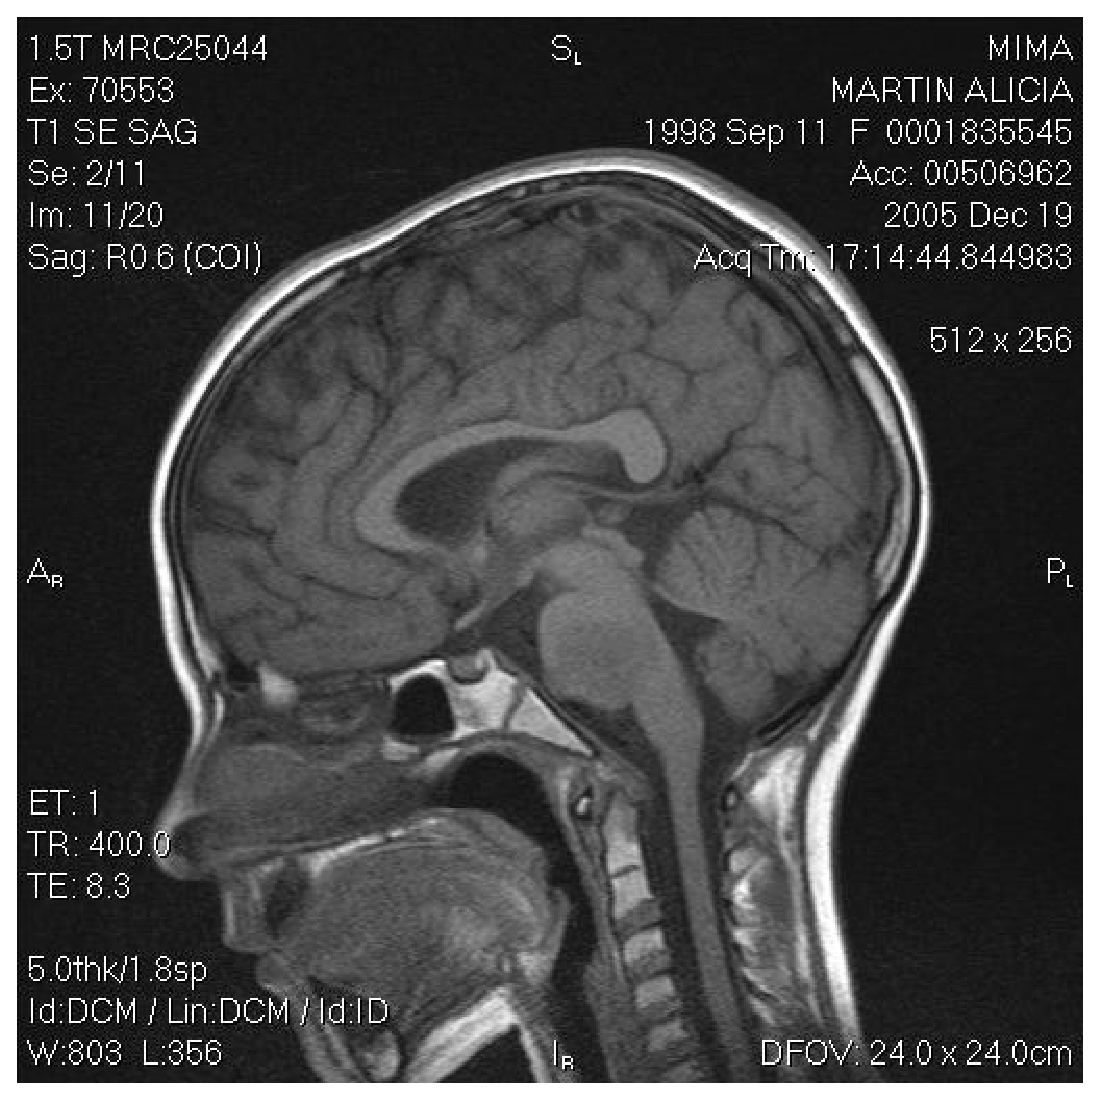
\epsfig{file=figure/MRI.eps, width=0.88\columnwidth}
}
% \subfloat[EEG]{
% \label{fig:medicalimage:eeg}
% 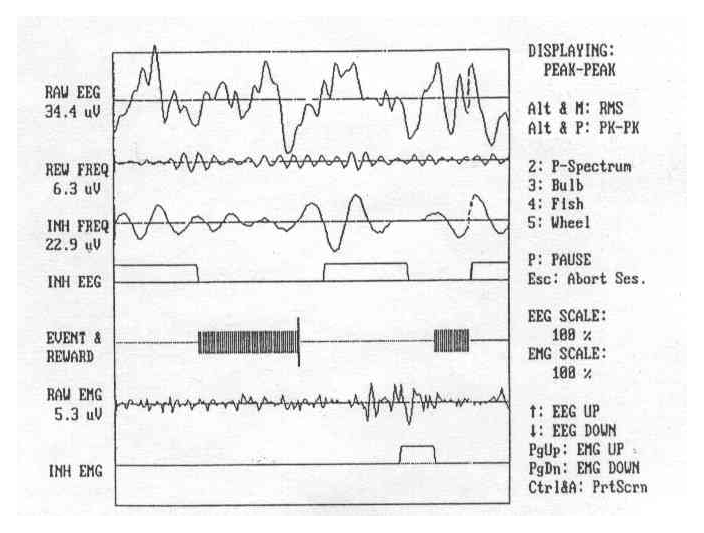
\epsfig{file=figure/EEG.eps, width=0.4\columnwidth}
% }
\caption{Examples of medical images with textual information.}
\label{fig:med-image-example}
\end{figure*}


% Part 2: Medical imaging, example image, raw OCR result (text + layout information)
% What's medical image, why important?
Due to ever evolving hardware and software, many medical images
such as electro-cardio graphs (ECGs), magnetic resonance imaging (MRI),
X-ray or ultrasound images are directly printed and stored
\st{in hard copy formats} \KQ{on paper}.
Medical images shown in \figref{fig:med-image-example}
contain a mix of graphics and text,
which include technical settings of the hardware used,
test measurements and simple diagnoses.
% TODO: why growing demand?
In order to build the manageable electronic medical records for patients,
there has been a growing demand for extracting such text-based
medical information from these medical images.
% What's the exmaple, and what's in the OCR output?
Given the ECG image in \figref{fig:running-ecg} as the running example,
existing OCR softwares are able to produce texts with spatial layout information,
indicating the positions of each recognized text in the image.
\figref{fig:running-xml} shows the raw OCR result produced by Tesseract,
where recognized texts are organized in the form of XML hierarchy of spans,
and we call them ``text boxes'' throughout this paper.
Texts are stored only in leaf text boxes,
and the layout information of each box is represented by
the coordinates (left, top, right, bottom) of its bounding box.
We use the term ``bounding box'' and ``zone'' interchangeably in this paper.
% TODO: Mention OCR error here??
It's worth mentioning that OCR softwares may generate incorrect texts.
for example, the original text ``Vent. rate'' in the image
is incorrectly recognized as ``Vcnt. rule'',
also ``63 bpm'' is recognized as ``53 bpm''.

\begin{figure*}[ht]
\centering
\epsfig{file=figure/running_ECG.eps, width=1.9\columnwidth}
\caption{An ECG with interesting text areas marked by red ovals.}
\label{fig:running-ecg}
\end{figure*}

% \begin{figure}[ht]
% \centering
% \subfigure[]{
% \label{fig:subfig:a}
% \begin{minipage}[b]{0.2\textwidth}
%\newsavebox{\firstlisting}
%\begin{lrbox}{\firstlisting}% Store first listing
%\begin{lstlisting}
%<p class='ocr_par' dir='ltr'>
%   <span class='ocr_line' id='line_2'>
%       <span class='ocrx_word' id='word_6'>Vent.</span> 
%       <span class='ocrx_word' id='word_7'>rate</span> 
%       <span class='ocrx_word' id='word_8'>65</span> 
%       <span class='ocrx_word' id='word_9'>bpm</span> 
%   </span>
%   <span class='ocr_line' id='line_3'>
%       <span class='ocrx_word' id='word_14'>PR</span> 
%       <span class='ocrx_word' id='word_15'>interval</span> 
%       <span class='ocrx_word' id='word_16'>162</span> 
%       <span class='ocrx_word' id='word_17'>ms</span> 
%   </span>
%    ...
%</p> 
%\end{lstlisting}
%\end{lrbox}
% \end{minipage}
% }
% \hspace[1in]
% \subfigure[]{
% % \label{fig:subfig:b}
% % \begin{minipage}[b]{0.2\textwidth}
\newsavebox{\secondlisting}
\begin{lrbox}{\secondlisting}
% \tiny
\begin{lstlisting}[basicstyle=\tiny,]
<p class="ocr_par" title="box 263 33 444 119">
   <span class="ocr_l" title="box 264 33 336 45">
       <span class="ocrx_w" title="box 264 33 299 45">Vcnt.</span> 
       <span class="ocrx_w" title="box 308 34 336 45">rule</span> 
   </span>
   <span class='ocr_l'>
       <span class="ocrx_w" title="box 264 51 283 64">PR</span> 
       <span class="ocrx_w" title="box 291 51 346 64">Interval</span> 
       <span class="ocrx_w" title="box 389 52 411 64">140</span> 
       <span class="ocrx_w" title="box 420 55 439 64">ms</span> 
   </span>
   ...
   </span>
</p>
<p class="ocr_p" dir="ltr">
   <span class="ocr_l">
       <span class="ocrx_w" title="box 396 33 411 45">53</span> 
       <span class="ocrx_w" title="box 420 33 449 48">bpm</span> 
   </span>
</p>
\end{lstlisting}
\end{lrbox}
% % \end{minipage}
% }

% \KZ{\figref{fig:ocrre} is output from what software? Tesseract?}
\begin{figure}[th]
%\subfloat[Image From Printer1]{
%\label{fig:ocrresub:a}
%\scalebox{0.8}{\usebox{\firstlisting}}} 
%\hfill
%\subfloat[Image From Printer2]{
\scalebox{0.6}{\usebox{\secondlisting}}
% \label{fig:ocrre}
\caption{Simplified OCR Results in XML for an ECG with Layout Information}
%\label{fig:ocrresub:b}
\label{fig:ocrre}
\end{figure}

% \lipsum[2]



% Part 3: Goal of this paper: structured information (kv pair) extraction
%         Challenge: hard to write wrapper (professional, not friendly)
%                    noisy information & OCR error
%         direct approach: zonal approaches
%         weakness: error propagation
% kernel: structure --> pure OCR (text, regex based approach) is not reliable: not in a same box
% ZOI approach: zonal / page layout: inaccurate position (between diff. figures), error propagation

% What's the final goal?
Apart from scanning the images into digital formats,
extracting the structured textual knowledge is more important for
building electronic medical records.
% Using examples to illustrate.
For example in \figref{fig:running-ecg},
we would like to extract the attribute-value pairs
(e.g., \textit{Vent. rate = 63 bpm}) and possibly other values such as
date (e.g., \textit{18-Nov-2010}) and time (e.g., \textit{9:13:02}),
since those values endow us with information of the particular patient.
% Informally define the task
% Obviously, raw OCR results didn't explicitly encode such structured knowledge,
Since discovering structured knowledge is beyond the scope of the OCR techniques,
the goal of this work is to provide a systematic solution,
which enables users to easily specify the data of interest in the images,
and automatically extract the corresponding textual values from raw OCR results.

There are some naive solutions for this information extraction task.
% Naive approach 1: regex matching
The first approach is to write regex expressions for each data to be extracted,
and apply them to different text boxes of the OCR result.
For example, using \textit{``Vent\textbackslash . rate .* bpm''}
to capture the target bpm value.
However, this approach suffers from two major problems.
First and obviously,
incorrect recognized texts lead to mismatches of regex rules.
Second, the hierarchical layout of OCR results are
not always organized in a human-readable manner.
For example in \figref{fig:running-xml}, the text ``Vcnt. rule'' and ``53 bpm''
are not automatically combined into the same text box, but are rather far apart.
In fact, the hierarchical layout is sensitive to many factors,
including color, contrast, accidental spots on the prints, or the angle of the scanner camera.
In this case, text-based regex rules are not well suited for medical images.
Besides, writing regex rules is too ad-hoc and non-trivial for end users.

% Naive approach 2: ZOI based
The second approach is more straightforward:
the user first annotates all the target zones of each
\st{desired data} \KQ{piece of data},
then simply conducts OCR on each fragment of images.
Though intuitive and easy to implement,
this approach highly relies on the the accuracy of carefully annotated zones,
either too larger or too smaller will affect the local OCR results.
% TODO: why?? I don't know.
In addition, there exists slight positional variations of target zones
between two images, even if they share the same format.
Therefore, the user have to annotate zones for every individual image,
which is tedious and labour intensive.

% Naive approach 3: page layout
Another alternative solution involves the page layout analysis technique~\cite{o1993document},
which includes identifying and organizing the textual regions
in the scanned image of a text document.
\figref{fig:running-page-layout} shows the page layout result of the running example.
In particular, the technique first segments textual zones (blue blocks) from
non-textual zones and arrange them in their original order,
then detects individual text unit (red lines under texts) in each zone.
% Then in order to analyze the logical roles of the text zones
% (titles, captions, footnotes, etc.), logical layout analysis
% is used for labeling the semantics of the text zones.
Page layout analysis is mainly used for analyzing the semantics of text zones
for plain text image documents,
and it encounters two problems when applied to this task.
% When applied to structured TIE on medical images,
% this technique encounters two problems.
First, it is based on the strong assumption that images of the same format
share the same structure of page layout result.
Noises in the image will affect the page layout result and
eventually generate totally error textual information.
Second, users must implement an addition wrapper to describe the location
(which texts in which regions) of each desired data.
This step highly depends on the detail result of page layout,
and writing such wrapper is almost intractable
for common users without expert knowledge.
% The page layout analysis technique is used to determine where the text
% resides on a page ,
% % By using page layout analysis technique, the hierarchy of physical components
% % can be generated and to match with the hierarchy of logical components, which
% % is predefined.
% The problem with applying
% such technique on medical images is that it creates so much noises
% that performance is ultimately affected.
% For medical images like ECG, useful information is often
% found in the small components of the image, while most of the images are
% regarded as noises.
% % check paper and more description, weakness, ref
\begin{figure*}[ht]
\centering
\epsfig{file=figure/page_layout.jpg, width=1.9\columnwidth}
\caption{Example result of page layout analysis.}
\label{fig:running-page-layout}
\end{figure*}

% Part 4: Our approach: ODL based (in fact we are writing a parser)
%         user-friendly;
%         present spatial information via element order (LR, UD) and rough spatial constraints, without too precise position
%         What's more: support error prompt and automatic correction based on OCR info & human correction.
% to solve: treat as an alignment problem: find the best alignment between var and box,
%       satisfying both data-level and spatial-level constraints.
% Challenge: How to measure the spatial-level fitness without hard code position information?
% Our approach: DSL-based, 3 advantages:
%    1. user-friendly: simple syntax to describe what's in the image, and what's the data-of-interest. all need: following left-to-right and top-to-bottom style.
%    2. robust and efficient alignment (fuzzy): leverage relative position and rough coordinates defined in ODL tolerant position delta
%    3. correction model: automatic made correction based on OCR and human feedbacks, and prompt errors to easily tell user what's wrong.

% 1. avoid what, our intuition is?
In order to attack the limitations of the above approaches,
We propose a domain-specific language for describing and extracting
structured textual information from the raw OCR data of medical images.
We call it OCR description language, or ODL in short.
The ODL parser then parses the raw OCR data
of the medical images according to the description,
and extracts structured textual data in a tree shape.
The ODL based solution has three major advantages.
% adv 1. user-friendly
First, compared with the previous methods, ODL is more user-friendly.
%Instead of writing ad-hoc wrappers,
Borrowing the syntax from PADS~\cite{fisher2005pads},
an ad-hoc data processing language,
ODL provides a concrete syntax which allows users to easily define
fixed strings and variables to be extracted,
customize compositions for better organizing structured data,
apply value constraints on variables, and rough spatial constraints on structures.
% adv 2. layout-aware
Second, the syntax of ODL is layout-aware.
Besides the explicit description of the bounding boxes of individual data,
ODL also implies the relative layout between different data elements,
which is based on the left-to-right and top-to-bottom data description manner.
Those rich layout information support the effectiveness of the ODL parser.
% so that ODL implies the relative layout between different elements.
% adv 3. robust and efficient alignment
Third, the parsing process of ODL is robust.
Intuitively, the process aims at finding the best alignments
between the data defined in ODL and the text boxes of the raw OCR result,
satisfying both value constraints,
spatial constraints and their relative layouts.
The fuzzy matching strategy is applied to tolerate
or even automatically correct recognition errors brought by OCR,
as well as slight layout variances between images.
Therefore, neither carefully annotated zones nor
perfect OCR recognitions are required in the extraction step.
% % adv 3. automatic correction
% Third, the extraction results of ODL can be further
% improved by automatic correction.
% ODL is able to detect imperfect alignments via
% string mismatches or constraint violations,
% and then prompts the user to manually correct prominent parsing errors.
% These manual corrections serve as incremental annotations,
% which update the fuzzy matching strategy, and produce better extraction results.

% Or: 1. user friendly; 2. rich spatial semantics (implicit, explicit); 3. fuzzy


% Part 5: In summary, bullets.
In summary, this paper makes three main contributions.
\begin{enumerate}
\item We design a declarative spatial data description language
for describing both spatial and value constraints in medical images,
which can be used to automatically generate parsers for
structured information extraction from these images.
The syntax of ODL can be generalized to
%textual information extraction on
the other image domains (\secref{sec:syntax});
\item We propose a robust ODL parser,
which builds the association between the text boxes from raw OCR results
and the corresponding description in ODL.
During the parsing phase, the parser is able to tolerate
the noises and errors brought by OCR recognition,
as well as inaccurate bounding boxes of input description (\secref{sec:parsing});
\item We conduct preliminary experimental studies of
structured information extraction on real ECG dataset.
The end-to-end evaluation result shows that our ODL based solution
consistently outperforms existing approaches.
Besides, the extraction accuracy further increases by 2\%,
given only a few number of manual corrections.
(\secref{sec:eval}).
\end{enumerate}


\section{Approach}
\label{sec:approach}
In this section, we first introduce the general framework of ChatMatch, which is modeled as
a sport tournament, then discuss some possible scoring functions that can be used by
the virtual judges in these competitions.

%Our whole evaluation framework consists of competition and scoring at three different levels. 
%The game level is at the bottom 
%and is played between two players. 
%Then comes the match level.
%To ensure the fairness of the game, 
%two games will be played between every two robots, 
%with each side starting a conversation.
%The result of two games determines the outcome of a match. 
%The tournament level is at the top
% and is composed of matches among different pairs of players. 

\subsection{Competition Protocol}
\label{sec:competition}
The competition takes place, from top to bottom, at tournament, match and
game levels.

\subsection*{Tournament Rules}
%\KZ{Give an overview of the how the tournament is run.}
We adopt a double round-robin 
sports tournament, where all bots participating in the competition 
converse directly with each other twice.
This is better than a knock-out system because it assesses a bot's ability to
deal with both strong and weak bots.
%For example, whether with weaker bots will induce them to make more mistakes or  how stronger bots will motivate their performance.
If we have $n$ chatbots players in our tournament, 
there will be $n\times (n-1) $ games in total.

\subsection*{Match Rules}
%\KZ{Talk about how the matches are administered. Just the procedure only.}
There are two chatbots competing in a single match. 
Each match consists of two games,
 started by a different bot. 
If we have $n$ bots in our tournaments, there 
will be ${n \choose 2}$ matches in total. 

\subsection*{Game Rules}
%\KZ{The procedure of the game. How each game is started and stopped.}
Each game is started by a player whose first utterance is provided by 
the system. The choice of the first utterance can be different 
depending on the domain of the bots and the ability we want to 
rank about the bots. For example, if we want to test 
the ability on movies, we can set a movie-related 
first utterance. 

During a game, there might be different ways to 
end the conversation. We can set a fixed number of exchanges 
or a terminating condition such as whether a bot makes a fatal error
or whether a certain score is reached.

\begin{table*}[th]
\centering
\scriptsize
\begin{tabular}{c|l|l}
%\hline
\toprule
\textbf{Dimension} & \textbf{Definition} &\textbf{Approach} \\ \midrule
Fluency  & Responses are fluent and natural.& Sentence perplexity. \\
Knowledge & Responses indicate the bot has the knowledge. & The number of times the bot expresses its ignorance to a question.\\
Proactivity & Responses actively proceed the conversation.&The number of times the bot raises a question. \\
Specificity & Responses are not generic.&The average of Distinct-1 and Distinct-2 \citep{li2015diversity}.\\
Diversity &Responses which are diverse and non-repetitive. &Repetition detection following the function in \algoref{algo:rep}. \\
Consistency &Responses do not contradict chat history. &Detect inconsistent questions following the function in \algoref{algo:inconsist}\\
Relevance & Responses are related to current context.& Ability to catch the relevant concept in chat history defined in \algoref{algo:bonus}. \\
\bottomrule
\end{tabular}
\caption{Seven evaluation dimensions.}
\label{tab:methods}
\end{table*}


\subsection{Scoring}
\label{sec:scoring}
\subsection*{Game-level Scoring}
%\KZ{Define a few functions: one to catch repeating, one to chat contradiction and one to catch long term memory.}

%Here we define the rules for recording points in one game between two bots. 
Inspired by \citet{finch2020towards}, 
we score each turn based on seven aspects of rules 
concerning \textit{consistency}, \textit{fluency}, \textit{knowledge}, \textit{specificity}, 
\textit{diversity}, \textit{relevance} and \textit{proactivity}. 
%As these seven metrics present a high level of 
%overlap among all distinct evaluation metrics used 
%during different process of human evaluation,
%we believe the combination of these seven distinct dimensions will be reliable. 
Finally, we sum up the scores for each bot for all the turns.
\tabref{tab:methods} documents the definition of these dimensions, which can all be scored
automatically.

%After finishing the calculation of the bonus and penalty scores for each turn, we obtain the scores of the two bots in a game with weighted sum according to \eqnref{eq:sum-up}

%\begin{equation}
%S(bot) = \sum_t - c\times C(t)  - r \times R(t) + b \times B(t)
%\label{eq:sum-up}
%\end{equation}
%$S$ denotes the total score gained by a bot for a game.
\begin{figure}[th]
        \centering
        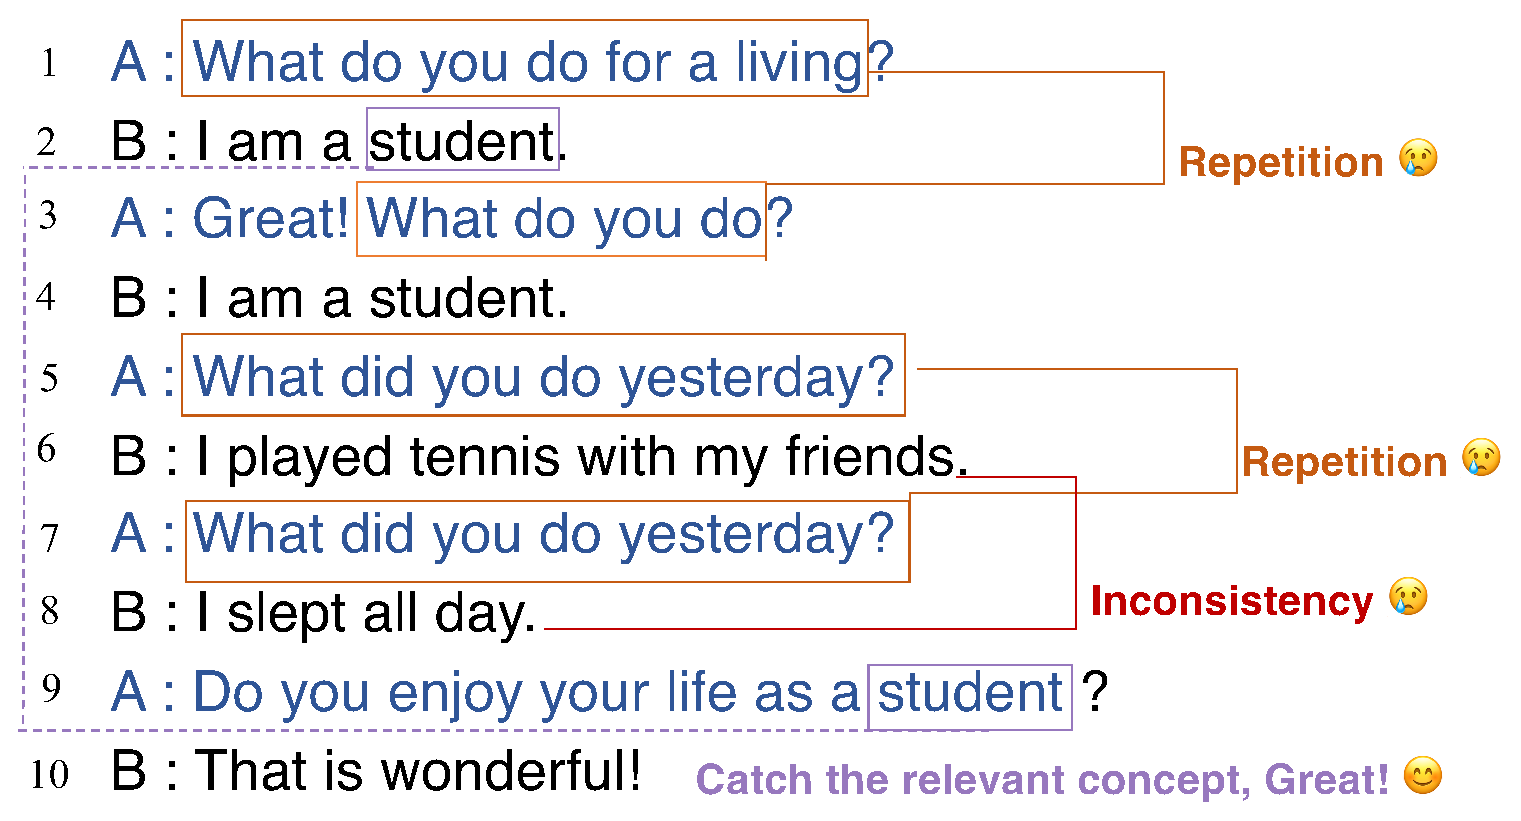
\includegraphics[width=0.95\columnwidth]{example2.eps}
        \caption{A chat snippet between two bots.}
        \label{fig:example}
\end{figure}

Fluency, Knowledge, Proactivity and Specificity are scored for each turn separately
and aggregated at the end of the conversation.
Detection for diversity, consistency and relevance are more involved and are explained
using \figref{fig:example}. 

As for diversity, at each turn $t$, we first check if there exists any repetitive question.  
We can easily find turn 3 and turn 7 repeated turn 1 and turn 5 
respectively. They will then be penalized one point for repetition. 
Repetition is not penalized if the previous turn is already 
marked as a repetitive question. For example, in \figref{fig:example}, 
although turn 4 is considered a repetition of turn 2,  
we are not going to penalize it as turn 3 is a repetitive question. 

The detection of inconsistency is always triggered after the detection of repeated questions. 
If the answers to the same questions are different, we will penalize the current turn, 
such as turn 8 in \figref{fig:example}.

We decide a repetition or an inconsistency by calculating the similarity of the two turns. 
We use a similarity function to complete the calculations, which we will 
discuss in \secref{sec:experiment}. The actual diversity and consistency scores
are the negation from the amount of repetition and inconsistency.

Relevance is assessed as a bonus to reward
a bot if it is able to memorize the important relevant concepts that have shown up 
before in the conversation. We sort the concepts that have shown up in 
chat history by their IDF scores. For example, in turn 9, $A$ 
mentions the concept word ``student'' presented by $B$ in turn 2. With this
turn, $A$ will win a bonus point.


The algorithms and notations for computing diviersty, consistency and relevance are included
in \tabref{tab:functions}, \algoref{algo:rep}, \algoref{algo:inconsist}, and \algoref{algo:bonus}. 

\begin{table}[th]
\centering
\small
\begin{tabular}{c|l}
%\hline
\toprule
\textbf{Notation} & \textbf{Description} \\ \midrule
$t$ & Current turn \\
$H(t)$  &  a list of history turns prior to $t$ \\
$Sim(x,y)$ & similarity between two turns $x$ and $y$ \\
$\sigma_r$ & Threshold for detecting repetition \\
$\sigma_c$ & Threshold for detecting consistency \\
$r$ & Weight for repetition \\
$c$ & Weight for inconsistency \\
$b$ & Weight for bonus \\
$d$ & Min distance between consecutive mentions \\
IDF list & List of lemma in chatlog sorted by IDF\\
$p$ & Percentage of important lemmas in IDF list\\
$R(t)$ &  Repetition penalty for turn $t$ \\
$C(t)$ &  Inconsistency penalty for turn $t$ \\ 
$B(t)$ &  Memory bonus for turn $t$ \\
$Rep(t)$ & A list of repeated turns for turn $t$ \\  
\bottomrule
\end{tabular}
\caption{
Functions and variables in algorithms.}
\label{tab:functions}
\end{table}

\begin{algorithm}[th]
\small
\caption{Scoring for Diversity}
\label{algo:rep}
\hspace*{0.02in} {\bf Input:}
 $t$, $H$, $Sim$, $\sigma_{r}$
; \hspace*{0.02in} {\bf Output: } 
 $R$;
\begin{algorithmic}[1]
\State //Starting to detect repetition
\For {$u$ in $H(t)$}
	\If {$Sim(t,u) \geq \sigma_{r}$}
		\State Add $u$ to $Rep(t)$
	\EndIf
\EndFor
    \If{$len(Rep(t))\geq 0$}
        \If{$t$ is a question and We can find a question in $Rep(t)$}
        \State $ R(t) \leftarrow  R(t) + 1$ 
        \Else
        \If {the previous turn of $t$ is not a repetitive question}
        \State $R(t)) \leftarrow R(t) + 1$ 
        \EndIf
        \EndIf
    \EndIf
\end{algorithmic}
\end{algorithm}


\begin{algorithm}[th]
\small
\caption{Scoring for Consistency}
\label{algo:inconsist}
\hspace*{0.02in} {\bf Input:}
$t$, $H$, $Sim$, $\sigma_{c}$
; \hspace*{0.02in} {\bf Output:  } 
 $C$;
\begin{algorithmic}[1]
\State // Inconsistency detection
 \If {previous turn of $p$ is a repetitive question} 
   \If{ the response $res$ to the question repeated by turn $p$ contradicts turn $i$ with $Sim(t, res) \leq \sigma_{c}$ }
    \State $C(t) \leftarrow C(t) + 1$
   \EndIf
  \EndIf
\end{algorithmic}
\end{algorithm}

\begin{algorithm}[th]
\small
\caption{Scoring for Relevance}
\label{algo:bonus}
\hspace*{0.02in} {\bf Input:}
$t$, $p$, $d$
; \hspace*{0.02in} {\bf Output:  } 
$B$;
\begin{algorithmic}[1]
\State // Assessing the ability of catching relevant concepts\\
$B(t) \leftarrow 0$
\For {all tokens $tk$ in current turn $t$}
 \If {$t$ - previous occurrence turn of $tk > d$ and $tk$ in the top $p\%$ of the IDF list of all tokens in the dialogue} 
   \State $B(t) \leftarrow 1$
  \EndIf
 \EndFor
\end{algorithmic}
\end{algorithm}

At the end of each game, each bot gets seven scores, one for each dimension.  
After pairwise comparison on individual dimension, a bot gains one point for win and zero point for a tie or lose.
The final score of each bot is determined by the sum of their individual scores.
%\KZ{Are these scores positive or negative? Comparable between bots?}

\subsubsection*{Match-level Scoring}
%\KZ{Use an equation to compute the final scores?}
One match which consists of two games, each started with a different bot, 
decides winning or losing between two bots.
For match-level scoring, we mimic the scoring rules of soccer tournament. 
For each match, $W$ points for the winner,  
$T$ points for a tie and 
$L$ points for the loser.
The value of $W$, $T$ and $L$ will be discussed in \secref{sec:ablation}. 

%\KZ{At the match level, we need to consider different starting context for the bots? I think we should present a few options for the reader and say that we are limited to these.}

\subsubsection*{Tournament-level Scoring}
%\KZ{Use an equation to compute the final scores?}
We count the points by simply summing up their scores gained in every match. Currently, several bots with the same final rank are tolerated. For future study, it's possible to mimic more detailed rules presented in sports match such as determine their ranking based on their win-loss relationship in the match between them.  
If they are still tied, we could propose an “overtime” for these two bots, one human judge may observe their performance and then make the decision of the game.
 %TODO: framework

%\section{Language for Speculation}\label{sec:language}

In this section, we define a language for speculation -- its syntax and
operational semantics. We also present illustrative examples.
% We start out by presenting the data model which is independent of the rest of the language.
% Then we describe the syntax and the operational semantics of the language,
% and finally we discuss the exit and commit semantics along with some examples
% to help understanding of the language.

\subsection{Data Model}\label{sec:datamodel}

In speculative nondeterminism, we assume a 
centralized data store acting as the primary programming environment. The implementation of this store is
not part of the language and therefore independent from the operational semantics of the language.
Here we present the abstract data model of the store that can be instantiated into different
concrete models.

A data model is a 6-tuple
$$\dm=\langle D_0,\alltype,\allop,\allstore,\vdash,\psi\rangle$$
where
\begin{description}
  \item[$D_0$] defines an empty data store, for example, 
    an empty set $\emptyset=\{\}$ or an empty multi-set $\lbb\rbb$.
  \item[$\alltype$] is the set of all possible data items in the data model.
    For example, $\alltype=\nat$ for data models such as a set of natural numbers. 
  \item[$\allop$] is the set of all data operations available in the data model.
  \item[$\allstore$] is the set of all possible data stores.
    For example, $\allstore=2^\nat$ for data models such as a set of natural numbers.
  \item[$\vdash\subseteq\allstore\times\allop$] is a binary relation denoted by $D\vdash d$.
    It defines when operation $d$ can be executed on the data store $D$.
    For example, if the operation $d$ has a precondition, $D\vdash d$ is
    true if and only if the condition is true when evaluated on the data store $D$.
  \item[$\psi:\allop\times\allstore\to\alltype\times\allstore$] is the transition function that
    defines the effect of data operations on the store. 
    In general, a data operation can do read, update, or both. 
    For read purpose, a data item $t\in\alltype$ in the data store must be returned from $\psi$. 
\end{description}

Next we give some examples of concrete data models under the above framework.

\subsubsection*{Tuple Space}

The idea of tuple space comes from Linda \cite{Gelernter85:Linda}, where
a tuple space is a multi-set of tuples that can be accessed concurrently.
A tuple is an ordered collection of fields. 
Agents can post their data to the tuple space in the form of tuples, and 
retrieve tuples as data from the tuple space that match a certain pattern.
There are three major operations in the tuple space data model:
(i) $\In$ reads and removes a tuple from a tuple space;
(ii) $\Out$ produces a tuple, writing it into a tuple space;
(iii) $\Rd$ non-destructively reads a tuple space and gets a copy of a tuple. 
Both $\In$ and $\Rd$ are blocking while $\Out$ is non-blocking.
Formal definitions and operational semantics for
the $\In/\Out/\Rd$ operations \cite{Ciancarini95}
can be easily adapted to this framework.

\subsubsection*{Key-value Store}

{\em Key-value store} is a mapping from keys 
to values, e.g.
$[a\mapsto 3, b\mapsto 5]$ is a key-value store
where the key $a$ gets value $3$ and $b$ gets $5$.
Typical data operations include: (i) creating a new key-value pair,
(ii) updating an existing key with a new value,
(iii) getting a value according to a key, and
(iv) removing a key and its corresponding value.
Conditional guards can also be combined with these data operations,
e.g., $a>4\Rightarrow b\gets 2$ waits (blocks) until
the condition $a>4$ is true in the store,
and then updates the value of $b$ to $2$.

\subsubsection*{Other Models}

Other more structured data models include relational data and logic programs.
Data operations are insertion and deletion of tuples/predicates. Applications
using these models are also typical.


\subsection{Syntax}\label{sec:syntax}

% \RY{explain syntax, examples and then semantics. The semantics needs to
% be more detailed in the explanation and motivate the definitions etc.,
% e.g. what does commit do, what is the effect of this particular commit.
% What does exit do - why not just exit immediately. Also commit and
% exit are not immediate, again this is because of what they do.
% The local transitions part seems messy with things which are not defined
% but used. \\
% Erlang style notation has to be briefly explained. Use the first
% 2 rules in fly for this.
% }

\begin{figure}
\centering
\begin{eqnarray*}
     \text{Agent } a & := & p:f ~~|~~ \exiting ~~|~~ \exited \\
   \text{Program } p & := & e ~~|~~ op.e ~~|~~ t.e ~~|~~ e_1.e_2 ~~|~~ \epsilon \\
\text{Operation } op & := & d ~~|~~ e_1\oplus e_2 ~~|~~ \cm ~~|~~ \cu ~~|~~ \exit \\
                     &    & \\
      \text{Tree } T & := & w ~~|~~ T_1\oplus_k T_2 \\
     \text{World } w & := & \langle A,D,S\rangle \\
    \text{Agents } A & := & [] ~~|~~ [a_1,\dots,a_m] \\
 \text{Snapshots } S & := & \emptyset ~~|~~ \{s_1,\dots,s_n\} \\
  \text{Snapshot } s & := & \langle k,v\rangle
\end{eqnarray*}
\caption{Syntax and Runtime Data Structures.
$f:\allstore\to\nat$ is a exit function.
$e$ denotes a local computation,
$t\in\alltype$ is the input for the local computation,
and $\epsilon$ is the end of a local computation.
Dot (.) in $p$ means sequencing.
$d\in\allop$ is a data operation while $D\in\allstore$ is a data store.
$k\in\nat$ is the identifier of an agent.
$v\in\nat$ is an exit value of an agent.
}\label{fig:syntax}
\end{figure}

The syntax of the language for speculation is 
formally described in Figure \ref{fig:syntax}. 
The idea is that we have two languages, one which deals with the speculative
computation, the other is a host language where the speculation constructs
are embedded within.
The host and speculation language are conceptually orthogonal though
in practice one would want them to be closer.
In our syntax, an agent consists of a program $p$ and an exit function $f$. 
In the syntax in Figure \ref{fig:syntax}, $e$ is used to denote a language
computation in the host language. Since the host language is arbitrary, we
only define a meta syntax here\footnote{
The syntax here is similar to \cite{Ciancarini95} which gives a semantics
of Linda embedded in a host language.
}
in that $e$ is meant to evolve to some other
local computation $e'$ outside our semantics.
We use $\epsilon$ to denote the end of such a local computation. 
There is a special syntax $t.e$ where $t$ is intended to be the
result of the data operation $d$ ($t$ is the result of transition function $\psi$).
The meaning is that $e$ is intended to consume the result $t$, which overloads,
the dot symbol.\footnote{
This is because $d$ is defined in the data model but divorced from the host
language, thus, there would be something in the host language to deal with
the result $t$.
}
During runtime, an agent can also switch to special states $\exiting$ and $\exit$, 
which will be explained in Section \ref{sec:semantics}. 

The top-level runtime data structure is the tree of worlds,
while a world is a triple of a list of agents $A$, 
a data store $D$, and a set of snapshots $S$. 
A snapshot $s=\langle k,v\rangle$ is used in exit 
where $k$ denotes the $k$-th agent and $v$ is the exit value. 
%

\begin{figure}[tb]
\begin{lstlisting}[caption={Speculation Example using Tuple Space. 
We use \texttt{(...)} to denote tuples and
$\lambda x.\varphi(x)$ denotes a condition for $\In$ and $\Rd$ on the specific field in a tuple, where $\varphi$ is the condition expression such as ``$x\texttt{=ac}\lor x\texttt{=cb}$'' which means $x$ is equal to either {\tt ac} or {\tt cb}.},label=lst:ts-example]
|$\In$|(ticket, ab)
|$\oplus$|
(|$\In$|(ticket, |$\lambda x.x\texttt{=ac}\lor x\texttt{=cb}$|) = (ticket, X)
 if X = ac
   |$\In$|(ticket, cb)
 else
   |$\In$|(ticket, ac))
\end{lstlisting}
\end{figure}

We use the tuple space data model throughout this paper 
due to its simplicity and expressive power.
In order to explain further, we rewrite Listing \ref{lst:intro-speculate}
concretely using the tuple space data model and show it in Listing \ref{lst:ts-example}.
%
We use this style of host language from now on to 
demonstrate local computations as well as to embed speculation primitives, where
(i) identifiers starting with lowercase letters are symbol literals,
(ii) identifiers starting with uppercase letters are variables,
(iii) equal sign (\texttt{=}) denotes pattern matching and binding,
(iv) variables are immutable after binding,
(v) $\lambda x.\varphi(x)$ is a first-class anonymous function 
taking $x$ as the parameter and evaluating $\varphi(x)$ as 
the result of the function on calling. 
%\KZ{But what's $x$? Its type?} 
Such features are derived from functional languages such as Haskell and Erlang. 
The choice of host language is primarily for ease of presentation,
since the speculative nondeterminism framework is independent of 
the host language and local computations.
However, we also have a prototype implementation in Erlang which also uses
Erlang as the host language, thus our syntax is most similar to Erlang.


\subsection{Examples}\label{sec:examples}

Next we describe some examples to help understanding the language.
% \XJ{TODO: exit function f inside at least one example}

% \subsubsection*{Bob and Jill (BJ)}

This example is about trading in an online marketplace. 
Photographer Bob wants to upgrade his equipment while Jill wants to downgrade.
Bob can either buy good lens and sell his average lens, 
or buy a good camera and sell his average camera.
Jill can either sell her good lens and buy an average camera, 
or sell her good camera and buy an average camera.
Listing \ref{lst:bob} and \ref{lst:jill} show the 
agent programs of Bob and Jill, respectively.
Both \texttt{buy()} and \texttt{sell()} are blocking and implemented in Listing \ref{lst:bjcom}.
\texttt{id()} returns a unique transaction number for each invocation.

\begin{figure}[tb]
\begin{lstlisting}[label=lst:bob,caption=Bob's Agent]
(buy(goodlens); sell(avglens); |$\cm$|)
|$\oplus$| (buy(goodcam); sell(avgcam); |$\cm$|)
|$\exit$|
\end{lstlisting}
\begin{lstlisting}[label=lst:jill,caption=Jill's Agent]
(sell(goodlens); buy(avgcam); |$\cm$|)
|$\oplus$| (buy(goodcam); buy(avgcam); |$\cm$|)
|$\exit$|
\end{lstlisting}
\begin{lstlisting}[label=lst:bjcom,caption=Common Routines for Trading]
sell(X): I = id(); |$\Out$|(sell,X,I); |$\In$|(buy,X,I)
buy(X):  (_,_,I) = |$\In$|(sell,X,_); |$\Out$|(buy,X,I)
\end{lstlisting}
\end{figure}

\TODO{include a tree of BJ?}


\subsubsection*{Flight Reservation (FR)}

In this example, we reuse the setting described in Section \ref{sec:intro}.
There are two types of agents: ticket sellers and ticket buyers. Ticket sellers are 
airlines which put up the air tickets for sale. Ticket buyers
are users who wants to travel from one city to another either on a direct
flight or by several hops. 
There are five cities ($a$ through $e$) 
and \figref{fig:flight} shows the flight connectivity map where 
an edge indicates that there is direct flight (in both directions) 
connecting two cities and the number on the edge is the price of the
flight. 
% For simplicity we ignore the flight times. 
In the seller program (Listing \ref{lst:tsell}), 
the ticket seller loops for several times, 
each time picks an edge randomly, 
and sells a ticket corresponding to that edge
(direction is also randomly selected). 
In the buyer program (Listing \ref{lst:tbuy}), 
every traveler (buyer) has exactly \$100 and tries to acquire enough tickets
that would fly him or her from $a$ to $e$ so long as the total price is 
less than \$100. In other words, $a\to b\to e$ 
and $a\to c\to d\to e$ are both possible routes.
{\tt fly()} is defined using pattern matching on parameters.
The base case is to arrive at the destination in the first fly, i.e.
{\tt fly(e, e, ...)} will evaluate to a symbol {\tt arrived} since 
the starting point is the destination. 
The recursive case is {\tt fly(a, e, ...)} will obtain unvisited neighbors and call {\tt try()}.
Note that using recursion with speculative nondeterminism is straightforward
as it is considered as a local computation and 
local computations are neither limited nor affected by our framework.

\begin{figure}[tb]
\centering
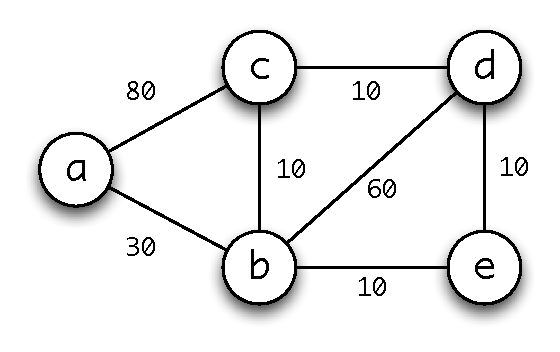
\epsfig{file=eps/flight-costs.eps,width=0.45\columnwidth}
\caption{Flight Map and Cost Between 5 Cities}
\label{fig:flight}
\end{figure}

\begin{figure}[tb]
\begin{lstlisting}[label=lst:tsell,caption=Ticket Seller's Agent. \texttt{[...]} denotes a list while \texttt{X[$i$]} is the $i$-th element of list \texttt{X}. \texttt{rand($m$)} returns a random integer between $0$ and $m$ (inclusive). \texttt{X.Y} denotes the concatenation of symbols so that \texttt{u.v} evaluates to \texttt{uv}.]
Ts = [[a,b,30],[a,c,80],[b,c,10],
      [b,d,60],[b,e,10],[c,d,10],[d,e,10]]
loop
  T = Ts[rand(6)]
  if rand(1) = 0
    |$\Out$|(ticket, T[0].T[1], T[2])
  else
    |$\Out$|(ticket, T[1].T[0], T[2])
|$\exit$|
\end{lstlisting}
\begin{lstlisting}[label=lst:tbuy,caption={Ticket Buyer's Agent. Both {\tt fly()} and {\tt try()} are defined using pattern matching on parameters. \texttt{[N:Ns]} denotes a list which has \texttt{N} as its head and \texttt{Ns} as its tail. Underscore (\texttt{\_}) matches anything in the context of pattern matching.}]
fly(X, X, Cash, V): arrived
fly(X, Y, Cash, V): Ns = unvisited_neighbors(X, V)
                    try(X, Ns, Y, Cash, V)

try(X, [N],    Y, Cash, V): buy(X, N, Y, Cash, V)
try(X, [N:Ns], Y, Cash, V): (buy(X, N, Y, Cash, V)
                            |$\oplus$|try(X, Ns, Y, Cash, V))
                            |$\cm$|

buy(X, N, Y, Cash, V):
  |$\In$|(ticket, X.N, |$\lambda x.x\le\texttt{Cash}$|) = (_, _, Cost)
  fly(N, Y, Cash - Cost, [N:V])

fly(a, e, 100, [a])
|$\exit$|
\end{lstlisting}
\vspace*{-5mm}
\end{figure}

\subsubsection*{Stock Trading (ST)}

In this example, we set up a mini stock market which follows the prices in the public exchange 
but is not openly available to the public. 
Traders can join the market at any time but their trades will not affect the public market.
Markets like this do exist in real life in the form of 
``Dark Pools''\cite{degryse2008shedding}  
which offers anonymous and private investors to
trade away from the public exachanges.

Our market starts with $N$ stocks, each has a fixed amount of shares dedicated for this market.
In general, each trader has a fixed amount of money in the beginning, 
and can buy (or sell) stocks from (or to) the market according to the public prices.
% Each trader also has a high watermark and a low watermark of cash.
% When the cash value is less than the low watermark (or greater than the high watermark), 
% the trader will keep selling (or buying) stocks in order to increase (or decrease) the cash value. 
% This strategy comes from real-world strategies where people want to control the risk.
% Different watermarks lead to different behaviors, and for this example, 
% the traders speculate to be either conservative or aggressive.
Listing \ref{lst:trader} shows the trader's agent program. 
Each trader trades several rounds until his cash value reaches the goal. 
For each round, the trader randomly picks a stock {\tt X}, buys it as much as possible, 
and waits for the price of {\tt X} to change. 
$\alpha$ is a value between 0 and 1 which indicates the profit/loss margin percentage. 
For example, if a trader buys {\tt X} at a price of {\tt P}, 
he sells it at a price of either higher than $(1+\alpha)\times{\tt P}$ (to profit)
or lower than $(1-\alpha)\times{\tt P}$ (to prevent further loss). 
Different $\alpha$ values lead to different trading behaviors, and for this example,
the traders speculate to be either 
conservative (smaller $\alpha$) or aggressive (larger $\alpha$).
Note that there is no atomicity guarantee between checking the price of a stock 
and actually buying it, which is also the behavior of a real market.
Also an intention to buy can be partially filled by the stock-serving agent
(see Listing \ref{lst:stock}).
The stock-serving agent also waits for price updating (i.e. {\tt (update, ...)})
from the public exchange in a realtime fashion. 

\begin{figure}[tb]
\begin{lstlisting}[label=lst:trader,caption={Trader's Agent. Numbers are irrelevant and just for illustration purposes.}]
Me     = unique_account_name
Stocks = [...]  // a list of stock names
Start  = 5000   // start with cash of $5000
Goal   = 5500   // the goal is to end up with $5500

trade(Cash, |$\alpha$|):
  X = Stocks[rand(N-1)]

  |$\Rd$|(price, X, _) = (_, _, P1)
  Q1 = |$\lfloor$|Cash / P1|$\rfloor$|
  |$\Out$|(buy, X, Q1, Me)
  |$\In$|(ack, Me, _, _) = (_, _, P2, Q2)
  C1 = Cash - P2 * Q2

  |$\Rd$|(price, X, |$\lambda x.x\ge(1+\alpha)\times{\tt P2}\lor x\le(1-\alpha)\times{\tt P2}$|)
  |$\Out$|(sell, X, Q2, Me)
  |$\In$|(ack, Me, _) = (_, _, P3)
  C2 = C1 + P3 * Q2

  if C2 < Goal
    trade(C2, |$\alpha$|)
  else
    |$\cm$|

trade(Start, 0.01) |$\oplus$| trade(Start, 0.05)
|$\exit$|
\end{lstlisting}
\begin{lstlisting}[label=lst:stock,caption=Stock-serving Agent. \texttt{P} is the current price of the stock while \texttt{Q} is the quantity of stocks available for sale.]
Me = unique_stock_name

serve(P, Q):
  case |$\In$|(_, Me, _, _)
    (update, _, NewPrc, _): |$\In$|(price, Me, _)
                            |$\Out$|(price, Me, NewPrc)
                            serve(NewPrc, Q)

    (buy, _, Q1, X): Q2 = min(Q1, Q)
                     |$\Out$|(ack, X, P, Q2)
                     serve(P, Q - Q2)
    
    (sell, _, Q2, X): |$\Out$|(ack, X, P)
                      serve(P, Q + Q2)

|$\Out$|(price, Me, Start_Price)
serve(Start_Price, Start_Quantity)
\end{lstlisting}
\vspace*{-6mm}
\end{figure}

\subsubsection*{Dining Philosophers (DP)}

% \begin{figure}[tb]
% \centering
% 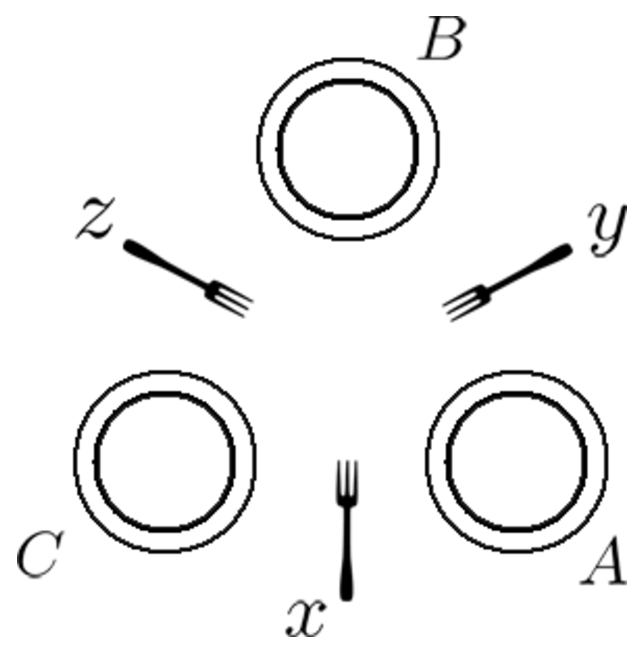
\epsfig{file=eps/dining.eps,width=0.3\columnwidth}
% \caption{Three Dining Philosophers Problem.
% $A,B,C$ are philosophers while $x,y,z$ are forks.}
% \label{fig:dining}
% \end{figure}

% \RY{can delete the figure. Listing 9 can be joined horizontally rather
% than vertically as now}

Consider the well-known ``Dining Philosophers Problem''
\cite{Dijkstra2002:Hierarchical} - there are three
philosophers $A$, $B$ and $C$, sitting around a dining table,
with three forks $x$, $y$ and $z$ between them.
This classic concurrency problem
shows that deadlock happens with certain sequences of acquiring the forks,
e.g., $A$ acquires $x$, $B$ acquires $y$ and then
$C$ acquires $z$. 
The classic solution to this problem is using a synchronization mechanism 
such as a counting semaphore, imposing a partial order on acquiring the forks, 
or requiring one philosopher to be asymmetric.
However, such kind of solution requires additional constraints to the problem. 
%
In this example, the speculation framework offers an alternative
solution which is purely based on the definition of the problem.
We extend the problem to $N$ dining philosophers 
sitting around a table with $N$ forks.
For simplicity, each philosopher has a unique index ranging from $0$ to $N-1$. 
Listing \ref{lst:dpinit} shows the initialization of data stores 
for dining philosophers.
Listing \ref{lst:dp} shows the agent program for dining philosophers.
\texttt{my\_index()} returns the index of the current philosopher.

\begin{figure}[tb]
\begin{lstlisting}[label=lst:dpinit,caption=Dining Philosophers (initialization)]
for I = 0 to N-1
  |$\Out$|(fork,I)
|$\exit$|
\end{lstlisting}
\begin{lstlisting}[label=lst:dp,caption={Dining Philosophers. \texttt{\%} denotes the modulo operation. {\tt ;} separates multiple statements in one line. $\Out$ is non-blocking in the tuple space data model, so we don't need choices for putting back forks.}]
L = my_index(); R = (L+1) % N
(|$\In$|(fork,L); |$\In$|(fork,R)) |$\oplus$| (|$\In$|(fork,R); |$\In$|(fork,L))
|$\cm$|
|$\Out$|(fork,L); |$\Out$|(fork,R)
|$\exit$|
\end{lstlisting}
\shrink
\shrink
\end{figure}

By using such kind of speculation, it can be guaranteed that 
there is always one world where nobody deadlocks. 
For example, assume $N=3$, the combination of the choices from three philosophers 
theoretically creates eight worlds as in Figure \ref{fig:diningrun} 
(though in practice some of the worlds may never be there due to pruning).

\begin{figure}
\centering\small
\Tree[.$\oplus_A$
    [.$\oplus_{B_1}$
        [.$\oplus_{C_1}$
            {$A\compact:-x$ \\ $\quad-y$ \\ $B\compact:-y$ \\ $\quad-z$ \\ $C\compact:-z$ \\ $\quad-x$ \\ $(w_1)$}
            {\bk$A\compact:-x$ \\ \bk$\quad-y$ \\ \bk$B\compact:-y$ \\ \bk$\quad-z$ \\ \bk$C\compact:-x$ \\ \bk$\quad-z$ \\ $(w_2)$}
        ][.$\oplus_{C_2}$
            {$A\compact:-x$ \\ $\quad-y$ \\ $B\compact:-z$ \\ $\quad-y$ \\ $C\compact:-z$ \\ $\quad-x$ \\ $(w_3)$}
            {\bk$A\compact:-x$ \\ \bk$\quad-y$ \\ \bk$B\compact:-z$ \\ \bk$\quad-y$ \\ \bk$C\compact:-x$ \\ \bk$\quad-z$ \\ $(w_4)$}
        ]
    ][.$\oplus_{C_3}$
        [.$\oplus_{B_2}$
            {$A\compact:-y$ \\ $\quad-x$ \\ $B\compact:-y$ \\ $\quad-z$ \\ $C\compact:-z$ \\ $\quad-x$ \\ $(w_5)$}
            {\bk$A\compact:-y$ \\ \bk$\quad-x$ \\ \bk$B\compact:-z$ \\ \bk$\quad-y$ \\ \bk$C\compact:-z$ \\ \bk$\quad-x$ \\ $(w_6)$}
        ][.$\oplus_{B_3}$
            {$A\compact:-y$ \\ $\quad-x$ \\ $B\compact:-y$ \\ $\quad-z$ \\ $C\compact:-x$ \\ $\quad-z$ \\ $(w_7)$}
            {\bk$A\compact:-y$ \\ \bk$\quad-x$ \\ \bk$B\compact:-z$ \\ \bk$\quad-y$ \\ \bk$C\compact:-x$ \\ \bk$\quad-z$ \\ $(w_8)$}
        ]
    ]
]
\caption{Three Dining Philosophers Problem (tree of choices). Minus sign ($-$) denotes taking the fork. Deadlock only happens in $w_1$ and $w_8$.}
\label{fig:diningrun}
\shrink
\end{figure}

There are many practical algorithms and applications (e.g., 2-phase locking)
that are special cases or extensions of the Dining Philosopher Problem (DPP). 
So we generalize DPP as follows.
\begin{definition}[Generalized Dining Philosopher Problem]
Given a set of resources $R$ which are available at the beginning, 
$n$ agents each interested in a subset of resources 
$R_i\subseteq R (1\le i\le n)$, and each agent is a two-phase process:
  \begin{enumerate}
    \item In the \emph{acquisition phase} the agent consumes every resource $r\in R_i$ in any order;
    \item In the \emph{release phase} the agent puts back every resource $r\in R_i$ in any order.
  \end{enumerate}
  $R_i$'s may overlap so the scheduler may produce a schedule which can cause deadlock 
among the agents.
\end{definition}

\begin{theorem} Generalized Dining Philosopher Problems do not deadlock 
using speculative nondeterminism.
\end{theorem}
\begin{proof}[Proof sketch]
% first show there is always a solution
First, we construct a combination of choices which will never deadlock. 
Fix an ordering of the elements in $R$, for example $r_1,r_2,\dots,r_m$ where $m=|R|$. 
For any agent $i$, it consumes $R_i$ in this fixed order. 
Then there will be races instead of deadlocks because there will not be the 
case that agent $i$ consumes $r_x$ and waits for $r_y$, and agent $j$ consumes
$r_y$ and waits for $r_x$ ($x<y$ and $y<x$ cannot be true at the same time). 
% then show the solution will not be pruned
Then it can be shown this combination will not be pruned by commits in an 
eventually blocking world due to the commit semantics described in rule \ref{rule:cm}. 
\end{proof}


\begin{figure}[ht!]
\centering
% TODO: use a tabular{cr} to format better
\flushright\fbox{Entrance transition: $T\|a\Longrightarrow T'$}
\[
  \tag{\sc Entrance1}\label{rule:entrance1}
  \langle A,D,S\rangle \| a \Longrightarrow \langle A+[a],D,S\rangle
\]
\[
  \tag{\sc Entrance2}\label{rule:entrance2}
  T_1\oplus_k T_2 \| a \Longrightarrow (T_1 \| a)\oplus_k (T_2 \| a)
\]
\flushright\fbox{Tree transition: $T\To T'$}
\[
  \tag{\sc Swap}\label{rule:swap}
  T_1\oplus_k T_2 \To T_2\oplus_k T_1
\]
\[
  \tag{\sc DataOp}\label{rule:dataop}
  \frac
  {A[k]=d.e:f \qquad D\vdash d \qquad \langle t,D'\rangle=\psi(d,D)}
  {\langle A,D,S\rangle \To \langle A[k\mapsto t.e:f], D', S\rangle}
\]
\[
  \tag{\sc Choice}\label{rule:choice}
  \frac
  {\begin{matrix}
    A[k]=(e_1\oplus e_2).e:f \\
    T_1=\langle A[k\mapsto e_1.e:f],D,S\rangle \\
    T_2=\langle A[k\mapsto e_2.e:f],D,S\rangle
   \end{matrix}}
  {\langle A,D,S\rangle \To T_1\oplus_k T_2}
\]
\[
  \tag{\sc Cm}\label{rule:cm}
  \frac
  {A[k]=\cm.e:f}
  {\langle A,D,S\rangle\oplus_k T \To \langle A[k\mapsto e:f],D,S\rangle}
\]
\[
  \tag{\sc Cu}\label{rule:cu}
  \frac
  {A[k]=\cu.e:f}
  {\langle A,D,S\rangle\oplus_k T \To T}
\]
\[
  \tag{\sc Exit1}\label{rule:exit1}
  \frac
  {A[k]=\exit.e :f \qquad s=\langle k,f(D)\rangle}
  {\langle A,D,S\rangle \To \langle A[k\mapsto\exiting],D,S\cup\{s\}\rangle}
\]
\[
  \tag{\sc Exit2}\label{rule:exit2}
  \frac
  {\begin{matrix}
    \forall w\in leaves(T): exiting(w,k) \land v = exitv(w,k)
   \end{matrix}}
  {T \To exit(T,k)}
\]
\[
  \tag{\sc Collapse}\label{rule:collapse}
  \frac
  {\begin{matrix}
    w \in leaves(T) \\
    \forall k: exiting(w,k) \lor exited(w,k)
   \end{matrix}}
  {T \To w}
\]
\flushright\fbox{Local computation transition: $e\computes e'$}
%\begin{align*}
\[
\begin{array}{llll}
  e &\computes op.e' \hspace*{5mm} &
  e &\computes \epsilon \\
  t.e &\computes e' &
  e_1.e_2 &\computes e_1'.e_2 \\
\end{array}
\]
%%  \epsilon.e &\computes e
%\end{align*}
\flushright\fbox{Helper functions}
\begin{gather*}
  \frac
  {T = T_1\oplus_k T_2}
  {leaves(T) = leaves(T_1)\uplus leaves(T_2)} \\
  leaves(w) = \lbb w\rbb \\
  \frac
  {w=\langle A,D,S\rangle \qquad \langle k,v\rangle\in S}
  {exitv(w,k) = v} \\
  \frac
  {w=\langle A,D,S\rangle}
  {exiting(w,k) = (A[k]=\exiting)} \\
  \frac
  {w=\langle A,D,S\rangle}
  {exited(w,k) = (A[k]=\exited)} \\
  \frac
  {T = T_1\oplus_i T_2}
  {exit(T,k) = exit(T_1,k)\oplus_i exit(T_2,k)} \\
  \frac
  {w=\langle A,D,S\rangle}
  {exit(w,k) = \langle A[k\mapsto\exited],D,S\rangle}
\end{gather*}
\caption{Semantics of the Speculation Language.
$[\dots]$ denotes a list,
$A[k]$ is the $k$-th element in list $A$, and
$A[k\mapsto x]$ denotes the updating of the $k$-th element to $x$.}
\label{fig:semantics}
\end{figure}

\subsection{Semantics}\label{sec:semantics}

The semantics of the speculation language is 
given in \figref{fig:semantics}. 

\paragraph*{Entrance}
New agents can dynamically enter the system at any time.
\ref{rule:entrance1} and \ref{rule:entrance2} the addition of
a new agent $a$ to the system (denoted $\|$). The Plus sign ($+$) 
denotes list concatenation. The whole tree is recursively traversed and $a$ is appended to the agent list in every world. 

\paragraph*{Choice Symmetry}
\ref{rule:swap} shows that the two branches of an interior node in the tree are treated equally.

\paragraph*{Data Operation}
An agent wants to execute operation $d$ on the data store $D$
(see \ref{rule:dataop}).
This transition first has to meet condition $D\vdash d$. 
The effect of $d$ on data store $D$ is defined by
the transition function $\psi$ in the data model and it only
affects the current world having store $D$
without affecting other worlds in the tree.
The result of $d$ is denoted is $t$ and provided to the remaining local 
computation $e$ as a parameter (denoted by the special syntax $t.e$). 
$t.e$ is not processed by the speculation framework, but 
activates the local computation $e$ and will eventually transform to another 
local computation $e'$ (i.e. $t.e\computes e'$). 

\paragraph*{Local Computation}
The local computation transition is simply a placeholder for
the semantics of the actual computation in the host language.
As that is orthogonal to our semantics, the details are left
unspecified. There is one special operation, $t.e$, which applies
the result of a data operation $t$ to some local computation $e$.
For example, it might be to store $t$ in a variable in the host language.
% \KZ{The following may need to be changed:\\
% We shall omit the details of the language in which 
% local computations are expressed and just assume that
% there exist a local computation transition $\computes$.
% From the perspective of the speculation framework, 
% the only thing that matters is the operation $op$ 
% produced by a local computation. 
% As shown in \figref{fig:semantics}, 
% a local computation $e$ transforms to $op.e'$ to 
% execute $op$ under the framework, or to $\epsilon$ to 
% finish execution. 
% After a data operation which reads something from the data store,
% a data item $t$ in the store is returned to the local computation $e$, 
% and further transforms to a new local computation $e'$, which is 
% $e$ parameterized by $t$. 
% $e_1.e_2$ denotes sequential execution of $e_1$ and $e_2$. 
% After $e_1$ transforms to $\epsilon$, $e_2$ starts execution 
% ($\epsilon.e\computes e$).
% }

\paragraph*{Choice and Commit}
Speculative nondeterminism provides for the creation and subsequent
pruning of choices. 
\ref{rule:choice} fires if an agent is reduced to a choice $(e_1\oplus e_2).e$, 
and it consumes the choice construct in the agent to split the current world into two
(i.e. $T_1$ and $T_2$). 
Section \ref{sec:commit} discusses further the ramifications of commit,
here, we start with first describing what the commit rules do.
When the $k$-th agent executes $\cm$ in a leaf world of the tree structure, 
as shown in rule \ref{rule:cm}, the other side of the choice (i.e. $T$) is pruned
only if the current choice node is $\oplus_k$. 
Similarly, $\cu$ is used where the agent wants to explicitly gives up the current choice branch,
so the current side of the choice is pruned, 
as shown in rule \ref{rule:cu}. 
$\cm$ and $\cu$ are symmetric and both of them are {\em commit} operators.
Commit of the $k$-th agent can only be executed in a world with $\oplus_k$ as its parent,
and it is blocking when the parent node is not $\oplus_k$.
%which makes the commit more localized and less aggressive. 
% This form of commit semantics is therefore known as {\em localized commit}.
%With this commit semantics, it only affects a small fraction of the whole tree. 
%Also it is possible to make pruning decisions locally, which makes it efficient. 

\paragraph*{Exit}
In general, a single agent will have many versions of itself executing
in all the multiple virtual worlds.
Thus, if it were simply to exit from all the worlds on the first
$\exit$ operation, this could lead to some form of data inconsistency.
We deal with this using the exit function $f$ specified by each agent which
allows an agent-specific consistency condition to be used.
Note that different agents may be interested in different aspects of the data store. 
When an agent exits, all the worlds should look the same from the perspective of that agent. 
However, another agent may not consider the worlds to be the 
same since it can have a different exit function. 
This also means that an agent properly exiting is only achieved when
the consistency requirement is obtained.

Rule \ref{rule:exit1} and \ref{rule:exit2} shows the exit semantics. 
\ref{rule:exit1} shows the case when an {\em instance} 
of the $k$-th agent reaches $\exit$ in a world. 
In this case, the exit function $f$ is applied to the current data store $D$ and a {\em snapshot} 
is created and added to $S$. 
 
The exit function $f$ takes a data store as input, and returns an integer as the evaluated result. 
The data store is just the one associated with the current world. 
According to the data store, the exit function is expected to produce an integer 
which can be a 0/1 indicator, a heuristic value, or an encoding of more complicated mathematical objects. 
For example, in the simplest case, $f(d)\equiv 1$ allows the agent to exit without any condition 
as long as it completes execution of all the operations in the program. 
The ability to return an integer provides more flexibility and enables 
complex exiting logic to be embedded in this exit function.

While taking a snapshot, 
the agent in that world switches to a special state $\exiting$.
\ref{rule:exit2} checks all the worlds in the tree. Only if (i) the $k$-th agent has 
switched to $\exiting$ state in all the worlds, and (ii) the exit value $v$ of the $k$-th agent 
is {\em identical} across all the worlds, 
then the $k$-th agent can exit from the worlds at the same time. 
For \ref{rule:exit2}, the exit value $v$, which can be thought of as the return value from
the speculative computation, will be eventually provided to 
a local computation $\tilde e$
which is completely outside the system of virtual worlds, 
and has no more speculation and data store operations. 
The idea of this type of consistent exit across all worlds is analogous
algebraic factorization, i.e.
$ab + ac = a(b+c)$.

\paragraph*{Collapse}
Note that commit is optional in an agent program, so the agents can 
let the tree expand without pruning, and finally leave the tree 
without reducing to one world. 
Therefore some agents may never exit due to the inconsistency of some worlds, 
even if all the agents have finished execution.
\ref{rule:collapse} handles this case 
to let these agents exit as well as to reclaim system resources. 
The system could employ a global collapse rule to pick any world where 
all agents have completed execution and reduce the tree to one world.
For \ref{rule:collapse}, the exit value for every agent $k$ is also returned in this way.
$\tilde e$ can make use of the exit value to extract what the agent concerns. 
%\KZ{Need to say exit is implicit if it's not added to the program?}

\paragraph*{Helper Functions}
We also define a set of helper functions to simplify the semantics. 
\begin{description}
\item[$leaves(T)$] returns a multi-set of the leaf worlds in tree $T$. 
\item[$exitv(w,k)$] retrieves the exit value, i.e. the evaluation result of the exit function, of the $k$-th agent in world $w$.
\item[$exiting(w,k)$] is a predicate indicating whether the $k$-th agent in world $w$ is in the special state of $\exiting$.
\item[$exited(w,k)$] is a predicate indicating whether the $k$-th agent in world $w$ is in the special state of $\exited$.
\item[$exit(T,k)$] switches the $k$-th agent in all the worlds in $T$ to the special state of $\exited$.
\end{description}

\subsection{More on Commit}\label{sec:commit}
Commit is a special and important operation in speculative nondeterminism because:
(i) it gives the agent the power to specify preferences among different choices,
e.g., in Listing \ref{lst:intro-commit-sleep}; 
(ii) it prunes some of the virtual worlds to make it easier for agents to exit
because the fewer remaining worlds means easier consistency checks,
and thus it improves the responsiveness and overall throughput of the system;
(iii) by pruning worlds, it also reclaims precious system resources such as
memory and CPU cycles, which is critical to the viability of the multi-world 
speculation , even though the naive combinatorial problem space is exponential and
prohibitive.

However, it is also important to understand that whenever commit is used and
pruning is done, potential solutions can be pruned away, and deadlock or blocking
may arise as a result. So from the system point of view, we design a commit
semantics that is {\em localized} and less aggressive because the scope of the pruning
is restricted to be of height 1 only and affects only a small fraction of
the whole tree (see Rule \ref{rule:cm}). This commit semantics is also
more efficient because pruning decisions are made locally. There are of course
other possible commit semantics \cite{JaffarYZ07} which are more eager in pruning. 
For example, one type of commit requires agent $T$ to commit in all left or right
subtree rooted at $\oplus_T$. These are either too aggressive and lose 
too many solutions or require coordination
among various worlds which is more costly to execute in practice.

From the programmer's point of view, she should use commit with care, knowing that
without commit, the multi-world space grows very quickly and the program probably
cannot scale, but with commit, the program could potentially lose valuable solution.
It makes more sense to put commit later rather than early in the choice. 
If one must put a commit in the middle of a sequence of operations like
$op_1.op_2.\cm.op_3.op_4$, she should ensure that the remaining operations
after $\cm$, i.e., $op_3$ and $op_4$, are not likely to block, 
e.g., when they are local computations.

%The commit semantics described in Section \ref{sec:semantics} 
%is called {\em localized commit} as it restricts
%the scope of pruning to be of height 1 only.  
%%$\cm$ by agent $X$ cannot
%%prune until the direct parent of the committed world is $\oplus_X$.
%%$\cu$ kills the current world immediately without coordination with other worlds.
%Besides localized commit, there is a number of other possible commit
%semantics \cite{JaffarYZ07}.
%They differ in their eagerness to prune the worlds.
%They are ordered roughly from the most eager to the most conservative:
%{\em absolutely eager commit}, {\em eager commit}, {\em coordinated commit}, 
%{\em late commit} and {\em no commit}. 
%




\section{Syntax of OCR Description Language}
\label{sec:syntax}

In this section, we introduce the OCR description language,
and explain what kind of structured data that ODL is able to describe.
The abstract syntax of ODL is formally described in \figref{fig:syntax}.
ODL is able to describe both structured data and
spatial layouts of textual information within the medical image.
In the following parts, we will discuss the ODL syntax and its type system in more detail.
% \newsavebox{\absfalign}
% \begin{lrbox}{\absfalign}
% % \fontsize{6pt}{7pt}\selectfont
% \begin{align*}
% \text{int} ::= ~&[-+]?[0-9]+ \\
% \text{float} ::= ~&[-+]?[0-9]*.[0-9]+ \\
% \text{num} ::= ~&int|float\\
% \text{len} ::= ~&num ~~ (pixel|cm) \\
% \text{coord} ::= ~&\langle len_1, ~~ len_2, ~~ len_3, ~~ len_4\rangle \\
% \text{bop} ::= ~&+|-|*|/|=|!=|<|>|<=|>=\\
% % \text{datatype} ::= 
% % ~&Oint(int, int)\\
% % |~& Ofloat(int, int, int, int)\\
% % |~& Ostring(string)\\
% \text{Value v} ::= 
% ~&() \\
% |~& int \\
% |~& float \\
% |~& string \\
% |~& len \\
% |~& coord \\
% % |~& {v_1, ~~ ..., ~ v_n}\\
% %|~& \{v_1 | v_2 | ... | v_n\}\\
% |~& \{v_1, ..., v_n\} \\
% \end{align*}
% \end{lrbox}

% \newsavebox{\abssalign}
% \begin{lrbox}{\abssalign}
% % \fontsize{6pt}{7pt}\selectfont
% \begin{align*}
% \text{Expression e} ::= 
% % |~& datatype ~~ x \tag{variable}\label{syntax:variable}\\
% ~&c \tag{constant}\label{syntax:constant}\\
% |~& x \tag{name}\label{syntax:name}\\
% % |~& nop ~~ e\\
% |~& e_0(e_1, e_2, ..., e_n) \tag{constraints} \label{syntax:constraints}\\
% % |~& \lambda x.e \tag{funciton}\label{syntax:function}\\
% % |~& e_1 ~~ e_2 \tag{apply}\label{syntax:apple}\\
% |~& hskip ~~e \tag{horizontal skip}\label{syntax:hskip}\\
% |~& vskip ~~e \tag{vertical skip}\label{syntax:vskip}\\
% |~& \{e_1 | e_2 | ... | e_n\} \tag{union}\label{syntax:union}\\
% % |~& \{e_1, ~~ ..., ~~ e_n\}\\
% % |~& e.i\\
% |~& \{e_1, ..., e_n\} \tag{struct}\label{syntax:struct}\\
% |~& e ~~ list \tag{list}\label{syntax:list}\\
% % |~& e_1[e_2] \tag{list element}\label{syntax:listele}\\
% |~& e ~~ as ~~ x \tag{blinding}\label{syntax:blinding}\\
% |~& e_1 ~~ bop ~~ e_2 \tag{binary operation}\label{syntax:bop}\\
% \end{align*}
% \end{lrbox}

% \begin{figure}[h]
% % \centering
% % \subfloat{\parbox{0.5\textwidth}{
% % {\usebox\absfalign}
% \begin{align*}
% \text{int} ::= ~&[-+]?[0-9]+ \\
% \text{float} ::= ~&[-+]?[0-9]*.[0-9]+ \\
% \text{num} ::= ~&int|float\\
% \text{len} ::= ~&num ~~ (pixel|cm) \\
% \text{coor} ::= ~&\langle len_1, ~~ len_2, ~~len_3, ~~ len_4\rangle \\
% \text{bop} ::= 
% ~&+|-|*|/\\
% |~& =|!=\\
% |~& <|>|<=|>=\\
% % \text{datatype} ::= 
% % ~&Oint(int, int)\\
% % |~& Ofloat(int, int, int, int)\\
% % |~& Ostring(string)\\
% \text{v} ::= 
% ~&() \\
% |~& int \\
% |~& float \\
% |~& string \\
% |~& len \\
% |~& coor \\
% % |~& {v_1, ~~ ..., ~ v_n}\\
% %|~& \{v_1 | v_2 | ... | v_n\}\\
% |~& \{v_1, ..., v_n\} \\
% % a = b\\
% % \end{align*}
% % }}
% % \end{subfloat}
% % \hfill
% % \subfloat{
% % \subfloat{\parbox{0.5\textwidth}{
% % {\usebox\abssalign}
% % \begin{align*}
% \text{e} ::= 
% % |~& datatype ~~ x \tag{variable}\label{syntax:variable}\\
% ~&c \tag{constant}\label{syntax:constant}\\
% |~& x \tag{name}\label{syntax:name}\\
% % |~& nop ~~ e\\
% |~& e_0(e_1, e_2, ..., e_n) \tag{constraints} \label{syntax:constraints}\\
% % |~& \lambda x.e \tag{funciton}\label{syntax:function}\\
% % |~& e_1 ~~ e_2 \tag{apply}\label{syntax:apple}\\
% |~& hskip ~~e \tag{horizontal skip}\label{syntax:hskip}\\
% |~& vskip ~~e \tag{vertical skip}\label{syntax:vskip}\\
% |~& \{e_1 | e_2 | ... | e_n\} \tag{union}\label{syntax:union}\\
% % |~& \{e_1, ~~ ..., ~~ e_n\}\\
% % |~& e.i\\
% |~& \{e_1, ..., e_n\} \tag{struct}\label{syntax:struct}\\
% |~& e ~~ list \tag{list}\label{syntax:list}\\
% % |~& e_1[e_2] \tag{list element}\label{syntax:listele}\\
% |~& e ~~ as ~~ x \tag{blinding}\label{syntax:blinding}\\
% |~& e_1 ~~ bop ~~ e_2 \tag{binary operation}\label{syntax:bop}\\
% % c = d\\
% % \text{Expression e} ::= 
% % % |~& datatype ~~ x \tag{variable}\label{syntax:variable}\\
% % ~&c\\
% % |~& x\\
% % % |~& nop ~~ e\\
% % |~& e_0(e_1, e_2, ..., e_n)\\
% % % |~& \lambda x.e \tag{funciton}\label{syntax:function}\\
% % % |~& e_1 ~~ e_2 \tag{apply}\label{syntax:apple}\\
% % |~& hskip ~~e\\
% % |~& vskip ~~e\\
% % |~& \{e_1 | e_2 | ... | e_n\}\\
% % % |~& \{e_1, ~~ ..., ~~ e_n\}\\
% % % |~& e.i\\
% % |~& \{e_1, ..., e_n\}\\
% % |~& e ~~ list\\
% % % |~& e_1[e_2] \tag{list element}\label{syntax:listele}\\
% % |~& e ~~ as ~~ x\\
% % |~& e_1 ~~ bop ~~ e_2\\
% \end{align*}
% % }}
% % \end{subfloat}
% \caption{Syntax}
% \label{fig:syntax}
% \end{figure}

\begin{figure}[h]
\small
\begin{align*}
\text{int} ::=~& \land-?\backslash d+\$\\
\text{float} ::=~& \land(-?\backslash d+)(.\backslash d+)?\$\\
\text{num} ::=~& int|float\\
\text{len} ::=~& num ~~ (pixel|cm)\\
\text{coor} ::=~& \langle len_1, len_2, len_3, len_4\rangle\\
\text{bop} ::= 
~& +|-|*|/\\
|~&=|!=\\
|~&<|>|<=|>=\\
% \text{datatype} ::= 
% ~&Oint(int, int)\\
% |~& Ofloat(int, int, int, int)\\
% |~& Ostring(string)\\
\text{v} ::=~& 
() \\
|~& int \\
|~& float \\
|~& string \\
|~& len \\
|~& coor \\
% |~& {v_1, ~~ ..., ~ v_n}\\
%|~& \{v_1 | v_2 | ... | v_n\}\\
|~& \{v_1, ..., v_n\} \\
%\end{align*}
%\begin{align*}
\text{e} ::= 
% |~& datatype ~~ x \tag{variable}\label{syntax:variable}\\
~& c \tag{constant}\label{syntax:constant}\\
|~& x \tag{name}\label{syntax:name}\\
% |~& nop ~~ e\\
|~& e_0(e_1, e_2, ..., e_n) \tag{constraints} \label{syntax:constraints}\\
% |~& \lambda x.e \tag{funciton}\label{syntax:function}\\
% |~& e_1 ~~ e_2 \tag{apply}\label{syntax:apple}\\
|~& hskip ~~e \tag{horizontal skip}\label{syntax:hskip}\\
|~& vskip ~~e \tag{vertical skip}\label{syntax:vskip}\\
|~& \{e_1 | e_2 | ... | e_n\} \tag{union}\label{syntax:union}\\
% |~& \{e_1, ~~ ..., ~~ e_n\}\\
% |~& e.i\\
|~& \{e_1, ..., e_n\} \tag{struct}\label{syntax:struct}\\
|~& e ~~ list \tag{list}\label{syntax:list}\\
% |~& e_1[e_2] \tag{list element}\label{syntax:listele}\\
|~& e ~~ as ~~ x \tag{blinding}\label{syntax:blinding}\\
|~& e_1 ~~ bop ~~ e_2 \tag{binary operation}\label{syntax:bop}\\
\end{align*}
\caption{Syntax}
\label{fig:syntax}
\end{figure}

\begin{figure}
\small
\begin{align*}
\text{t}::=~&unit\\
|~&int\\
|~&float\\
|~&len\\
%\end{align*}
%\begin{align*}
|~&\langle len, ~~ len, ~~ len, ~~ len\rangle\\
% &|~&t_1 \rightarrow t_2\\
|~&\{t_1 + t_2 + ... + t_n\}\\
|~&\{l_1 : t_1, ~~ ..., ~~ l_n : t_n\}\\
|~&t ~~ list\\
\end{align*}
\caption{ODL Data Types}\label{fig:type}
\end{figure}





% \KZ{Make \figref{fig:syntax} double column and more compact.}



\subsection{Primitive Expressions}
According to the abstract syntax, we start from the most primitive expressions
that ODL can describe: \textit{constant} and \textit{variable}.
Constants represent fixed-valued strings or numerical values to be recognized from the image.
For example in \figref{fig:running-odl-abstract}, ``Vent. rate'' and ``mm/mV''
are constant expressions, as they always occur in all ECGs of the same format.
% Constants are usually markers or delimiters in semi-structured data formats.
On the other hand, primitive variables represent numerical (int or float) values
varied in different images.
In \figref{fig:running-odl-abstract}, the variable $vr$ represents the
numerical value of ``Vent. rate''.%, which varies by different patients.
%Variables usually have a numeric type (int or float),
%and sometimes users know the constraints of its data field.
It's worth mentioning that,
the reason we specially define constants in ODL is to
enrich the relative layout information between different expressions,
so that the parser can locate the variables in the image more accurately.

\subsection{Spatial Expressions}
Spatial description expressions include \textit{hskip len} and \textit{vskip len}.
% These two expressions explicitly encode horizontal and vertical
% spacing information in the images, and we mainly explain the former one.
As shown in \figref{fig:running-ecg}, there has a large horizontal margin
between ``Vent. rate'' and ``63 bpm'', hence we can use \textit{hskip len} to
explicitly and approximately describe such horizontal margin
between the previous and next expressions.
% we can explain why needed here, because not all places have hskip/vskip.
The size of margin is determined by $len$, which has two parts:
the length value and its measurement unit.
Units can be the absolute pixel, or what are more encouraged,
the percentage of width ($w$) or height ($h$) of the image.
Besides, \textbackslash t stands for a special margin size,
which equals to the average width of 4 Latin characters.
We can easily estimate this value via the width of each text box
in the raw OCR results.
Similarly, \textit{vskip len} explicitly describes the vertical margin
between expressions, and \textbackslash n stands for the average height
of one Latin character.

\subsection{Composition}
Compositions are compound expressions constructed from other expressions.
These include \textit{union}, \textit{struct}, \textit{list}, \textit{binding}, \textit{bop} and \textit{constraint}.

The first three compositions define more structured and
complex type expressions.
The \textit{union} expression means there exists
multiple potential data or spatial expressions.
For example, the union description of $month\_str$ is the enumeration
of all abbreviations of different months.
The \textit{struct} expression is used to describe
an expression with multiple sub-expressions.
All sub-expressions must be described sequentially,
following the left-to-right then top-to-bottom manner.
As another example in \figref{fig:running-odl-surface},
the struct description of $triple\_t$ contains
the constant attribute name, spacing,
variable value and constant unit listed from left to right.
The \textit{list} expression indicates that a sequence of similar data or
the same spatial expressions should be applied multiple times.
In the example, \textit{vskip \textbackslash n list} represents several
blank lines between the data of interpretation and parameters in the images.

The function of \textit{binding} is to give a variable name \textit{x} to
the composition expression \textit{e}, so that each expression has an identifier
in the output parsing tree.
The function of \textit{bop} supports basic binary operations between numerical
values in the ODL.
These two expressions are designed to simplify the description of ODL.

Finally, the \textit{constraint} expression in ODL consists of two categories:
value constraints and spatial constraints.
Value constraints can be applied to the primitive variable,
indicating its type and value range, if the user knows in prior.
Since variables are usually numerical, two value constraints are available:
$x(int, v_{min}, v_{max})$ and
$x(float, length, precision, v_{min}, v_{max})$.
For example in \figref{fig:running-odl-abstract},
$day(int, 1, 31)$ constrains the variable to be an integer ranging from 1 to 31;
$p2(float, 3, 1)$ constrains the variable to be a floating number in length 3
and precision 1, without range limits.
Spatial constraints have the form $e(coor)$,
which can be applied to any expression,
and restrict the areas that corresponding data resides in the image.
Such positions in ODL are represented by $coor$, the 4-tuple of
left, top, right, bottom coordinates.
As shown in \figref{fig:running-odl-abstract}, spatial constraints
are applied to several structs: $time$, $tri$ and $inter$.
These constraints are rather rough and large,
as users are encouraged to give larger spatial constraints
if they are not so sure of the exact bounding boxes.


\subsection{Type System}

% In ODL, we can assign a types to every expression.
% We set up some rules determining types for expressions,
% which make up a complete type system.
The inductive typing rules of ODL is shown in \figref{fig:typingrule}.
% The type system of ODL is shown in \figref{fig:type} and \figref{fig:typingrule}.
% \figref{fig:type} shows the basic principles for determining types and
% \figref{fig:typingrule} extends it by providing inductive typing rules.
\textit{T-VARIABLE} indicates that the type of \textit{variable} is
based on the type of name in the typing context.
\textit{T-INT ARITH}, \textit{T-INT REL}, \textit{T-FLOAT ARITH} and
\textit{T-FLOAT REL} indicate that the two expressions of the \textit{bop}
are of the same type (int or float), and the final type of the \textit{bop}
expression is based on the binary operation.
\textit{T-CONSTRAINT} indicates that the final type of the \textit{constraints} expression is always the same as the original expression $e_0$.
\textit{T-HSKIP} and \textit{T-VSKIP} indicate that the spatial parameter $e$
is of the \textit{len} type, and the final types of these two expressions
should be \textit{unit}.
The last three of the typing rules are for
the \textit{union}, \textit{struct} and \textit{list} expressions, respectively.

% \begin{figure}[ht]
% % \centering
% \begin{minipage}{0.4\columnwidth}
% \begin{align*}
% \text{t}::=~&unit\\
% |~&int\\
% |~&float\\
% |~&len\\
% \end{align*}
% \end{minipage}
% \begin{minipage}{0.4\columnwidth}
% \begin{align*}
% |~&\langle len, ~~ len, ~~ len, ~~ len\rangle\\
% % &|~&t_1 \rightarrow t_2\\
% |~&t_1 + ... + t_n\\
% |~&t_1 * ... * t_n\\
% |~&t ~~ list\\
% \end{align*}
% \end{minipage}
% \caption{ODL Data Types}\label{fig:type}
% \end{figure}

\begin{figure}[ht]
% \centering
\begin{align*}
  \tag{T-VARIABLE}
  &\frac
  {\Gamma(x)=t}
  {\Gamma \vdash x:t}\\
  \tag{T-INT ARITH}
  &\frac
  {\Gamma \vdash e_1:int ~~ \Gamma \vdash e_2:int ~~ bop \in \{+,-,*,/,\%\}}
  % bop \in \{+,-,*,/,\%, =, !=, >, <, <=, >=\}
  {\Gamma \vdash e_1 ~~ bop ~~ e_2 :int} \\
  \tag{T-INT REL}
  &\frac
  {\Gamma \vdash e_1:int ~~ \Gamma \vdash e_2:int ~~ bop \in \{=, !=, <, >, <=, >=\}}
  % bop \in \{+,-,*,/,\%, =, !=, >, <, <=, >=\}
  {\Gamma \vdash e_1 ~~ bop ~~ e_2 :bool} \\
  \tag{T-FLOAT ARITH}
  &\frac
  {\Gamma \vdash e_1:float ~~ \Gamma \vdash e_2:float ~~ bop \in \{+,-,*,/,\%\}}
  % bop \in \{+,-,*,/,\%, =, !=, >, <, <=, >=\}
  {\Gamma \vdash e_1 ~~ bop ~~ e_2 :float}\\
  \tag{T-FLOAT REL}
  &\frac
  {\Gamma \vdash e_1:float ~~ \Gamma \vdash e_2:float ~~ bop \in \{=, !=, <, >, <=, >=\}}
  % bop \in \{+,-,*,/,\%, =, !=, >, <, <=, >=\}
  {\Gamma \vdash e_1 ~~ bop ~~ e_2 :bool}\\
  \tag{T-CONSTRAINT}
  &\frac
  {\Gamma \vdash e_0:t_0, \Gamma \vdash e_1:t_1, ..., \Gamma \vdash e_n:t_n}
  {\Gamma \vdash e_0(e_1, e_2, ..., e_n):t_0}\\
  % \tag{T-FUNCTION}
  % &\frac
  % {\Gamma[x:t_1] \vdash e:t_2}
  % {\Gamma \vdash fn ~~ x=> e:t_1 \rightarrow t_2} \\
  \tag{T-HSKIP}
  &\frac
  {\Gamma \vdash e:len}
  {\Gamma \vdash hskip ~~ e:unit}\\
  \tag{T-VSKIP}
  &\frac
  {\Gamma \vdash e:len}
  {\Gamma \vdash vskip ~~ e:unit}\\
  \tag{T-UNION}
  &\frac
  {for ~~ each ~~ i ~~ \Gamma \vdash e_i:t_i }
  {\Gamma \vdash \{e_1|...|e_n\}:t_1+...+t_n}\\
  \tag{T-STRUCT}
  &\frac
  {for ~~ each ~~ i ~~ \Gamma \vdash e_i:t_i }
  {\Gamma \vdash \{e_1, ..., e_n\}:t_1*...*t_n}\\
  % \tag{T-UNION}
  % &\frac
  % {for ~~ each ~~ i ~~ \Gamma \vdash e_i:t_i }
  % {\Gamma \vdash \{e_1|...|e_n\}:t_1+...+t_n}\\
  \tag{T-LIST}
  &\frac
  {\Gamma \vdash e:t}
  {\Gamma \vdash e~~list:t~~list}\\
  % \tag{T-LIST ELEMENT}
  % &\frac
  % {\Gamma \vdash e_1:t~~list ~~ \Gamma \vdash e_2:int}
  % {\Gamma \vdash e_1[e_2]:t}\\
\end{align*}
\caption{Inductive typing rules of ODL.}\label{fig:typingrule}
\end{figure}


% \textit{unit} type are for the
% expression of \textit{()} value. \textit{int}, \textit{float} and \textit{float} are types
% of the expressions that can be parsed into these type of values. \textit{len} is
% the type of \textit{len} value. The rest four kinds of types are the combination of
% all the types. \textit{$\langle len ~~ len, ~~ len, ~~ len\rangle$} is the type for
% \textit{coord}. \textit{$\{t_1 + t_2 + ... + t_n\}$} is the type for \textit{union} expression, which
% means the type of the value of \textit{union} can be any type of the components of the expression.
% \textit{$\{l_1 : t_1, ~~ ..., ~~ l_n : t_n\}$} is the type for \textit{struct}. All the types of
% the subexpressions in \textit{struct} are recorded. Finally, \textit{t ~~ list} is the type for
% \textit{list}. \textit{list} is made up of a sequence of the expressions in the same type.
% In \figref{fig:typingrule}, the detailed typing rules are described. Other than the types
% of the expressions, \textit{T-INT ARITH}, \textit{T-INT REL}, \textit{T-FLOAT ARITH} and \textit{T-FLOAT REL}
% indicate that the two expressions of the \textit{bop} shown be in the same type, int or float, and
% the final type of the \textit{bop} expression is based on the binary operation. \textit{T-CONSTRAINS}
% indicates that the types of the expressions in the constraints have nothing to do with the
% final type of the \textit{constraints} expression.

% \section{Circuit Component and Generator}\label{sec:syntax}
We explored the reconfigurable circuit component in AES architecture and designed a
new language construct $map$ accordingly to describe it, which portraits the computation 
meaning of the reconfigurable structure.

The $map$ is used to model the circuit that does some operations upon a list of data. It's also similar to higher order function "$map$" in Haskell. In Haskell, $map$ takes two inputs - a function, and a list. It then applies this function to every element in the list. In Verilog we don't have list type. However we can view a $reg$ or $wire$ as a bit list, and every time we applies the function (actually we should call it a $module$ in circuit design) to a slice of the bits. Figure \ref{fig-map} shows the $map$ structure, as an example, we can think  "Module" has the functionality that adds 1 to the input data list. Here comes the syntax of $map$:

\begin{verbatim}
         map(md,data,datalen,maplen)
\end{verbatim}
where $md$ is a module identifier, $data$ is the bit-list name (variable name of a $reg$ or $wire$), $datalen$ is the length of the bit-list and $maplen$ is the length of the bit slice that applied to the module each time.
%\vspace{-2ex}
\begin{figure}[ht]
\centering
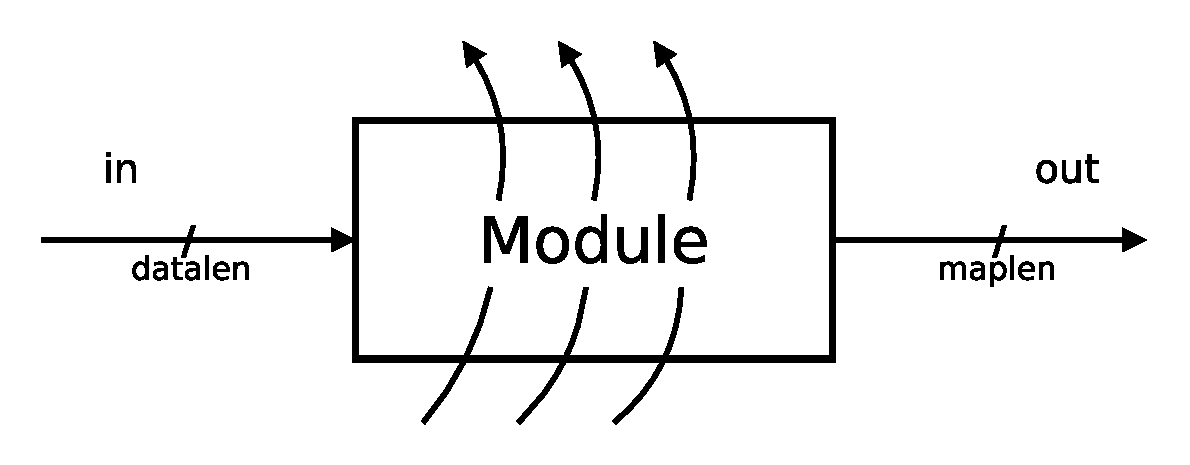
\epsfig{file=map.eps,width=0.5\columnwidth}
%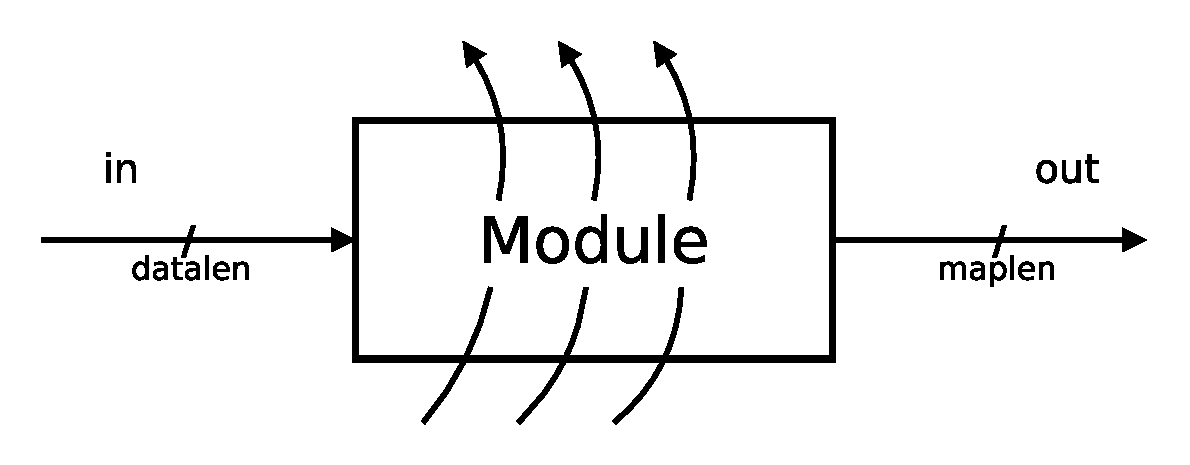
\includegraphics[scale=.5]{map}
%\vspace{-2ex}
\caption{Map Circuit Structure}
\label{fig-map}
\end{figure}

%\input{robust_matching}

\section{Robust ODL Parser}
\label{sec:parsing}

In this section, we focus on the ODL parser,
which is the core of the entire information extraction system.
% we focus on the process of structured textual information extraction,
% which is the kernel part of the entire system.
We first describe the semantics that the parser is used for generating
parsing trees based on the ODL specification.
Afterwards, we describe the detail of the fuzzy matching strategy
and the automatic correction model.

\subsection{Semantics of the ODL Parser}
% 1. in general, what's the parsing process
Referring to \figref{fig:running-parsing-tree},
the parsing process evaluates the entire data expression of ODL
into hierarchical texts organized by the parsing tree,
defined as $T = (node, [T_1, ..., T_n])$,
where $T_i$ is the $i$-th sub-tree of $T$.
The leaf nodes of $T$ are $(e, text)$ pairs representing the alignment
between some primitive expression and its corresponding text,
and non-leaf nodes are always the variable names $x$.

% 2. recursive process
Since the entire expression has a complex structure,
the evaluation is conducted recursively:
it first evaluates each sub-expression, and then composes multiple parsing trees
into a large one.
So the semantics of the parser consists of two parts:
the evaluation rules for non-compositional expressions
(constants, primitive variables and spatial expressions),
and the inductive evaluation rules for compositional expressions.

% talk about basic
% \subsubsection{Evaluation Rules for Non-compositional Expressions}
The most basic rule is for evaluating constants (or primitive variables):
given the OCR data $D$ and the constant (or primitive variable) $e$ in ODL,
searching all possible alignments between $e$ and some text box $d \in D$.
During the whole parsing process, the parser maintains an environment
$E = (x_0, y_0, x_1, y_1, x_{cr}, y_{cr})$,
which contains the coordinates of the searching area,
as well as a cursor ($x_{cr}$, $y_{cr}$).
The cursor is a reference point, indicating the rough position
that the desired text box resides.
By default, the searching area is the whole image,
and the cursor is at the top-left corner.
The relative layout in ODL is represented in a
left-to-right then top-to-bottom manner,
thus the text box $d$ becomes a candidate alignment of $e$,
if it's within the searching area,
and not located in the top-left side of the cursor.
The following $InBound$ function defines such rule:
\begin{equation}
  \begin{aligned}
      InBound(D, E) & = \{d \in D\ |\ \\
      & E.x_0 \leq d.x_0 \leq d.x_1 \leq E.x_1 \\
      \land &
      E.y_0 \leq d.y_0 \leq d.y_1 \leq E.y_1 \\
      \land & \lnot
      ( d.x_1 \leq E.x_{cr} \land d.y_1 \leq E.y_{cr} )
      \}. \\
  \end{aligned}
\end{equation}
With the environment $E$ provided,
the parser enumerates all candidate text boxes,
and use a boolean match function $Match(e, d; E)$ to
judge whether an alignment exists between $d$ and
the constant (or primitive variable) $e$.
Intuitively, $d$ is a valid match of $e$,
if its text is close to the constraints of $e$,
and it's located near the cursor ($E.x_{cr}, E.y_{cr}$).
For a better flow of explanation, the formal definition of the match function
will be given in the next section.
If matches, a new parsing tree $T=((e, d.text), [])$ is generated,
which has a single node without any children.
Besides, both $D$ and $E$ need to be changed, so that the parser
can work on the alignment of the subsequent expressions in ODL.
Following the relative layout of expressions,
the cursor is moved to the top-right corner of the box:
$E' = Move(E, d)$, and $d$ is removed from $D$,
as one text box can be aligned at most once: $D' = D - \{d\}$.
\equref{equ:semantic-operations} defines a series of functions
that changes the environment, which are used in different evaluation rules.
In which, $c$ is short for $coor$.
\begin{equation}
  \begin{aligned}
    Move(E, d) = & (E.x_0, E.y_0, E.x_1, E.y_1, d.x_1, d.y_0), \\
    Hskip(E, len) = & (E.x_0, E.y_0, E.x_1, E.y_1, E.x_{cr}+len, E.y_{cr}), \\
    Vskip(E, len) = & (E.x_0, E.y_0, E.x_1, E.y_1, E.x_0, E.y_{cr}+len), \\
    Restrict(c) = & (c.x_0, c.y_0, c.x_1, c.y_1, c.x_0, c.y_0). \\
  \end{aligned}
  \label{equ:semantic-operations}
\end{equation}

The tuple $(T, E, D)$ is called a \textit{parsing state},
which records the partial parsing tree,
the environment information and the remaining text boxes.
Since there exist multiple candidate text boxes for alignment,
given $E$ and $D$, $e$ will be evaluated into a set of parsing states,
written in the following judgment form:
\begin{equation}
  E,D;e \Downarrow \bigcup_{i} \{(T_i, E'_i, D'_i)\}.
\end{equation}


\begin{figure*}[ht!]
% \[
%   {\rm Judgment~ Form:}~~ E,D;e \Downarrow (D';parse\_tree)list
%   \label{semantic:judegement}
% \]
% where E is environment, D and D' are input\_data, C records the position of the cursor.
\begin{gather*}
  \tag{\sc E-Empty}\label{rule:empty}
  \frac
  {InBound(D,E)=\emptyset}
  {E,D;e \Downarrow \{(((e, Nil), []), E, D)\}}\\
  \tag{\sc E-PRIM1}\label{rule:c1}
  \frac
  {d \in InBound(D,E), Match(e, d; E)=True, E'=Move(E, d) ~~ E',D-\{d\};e \Downarrow r}
  {E,D;e \Downarrow r \cup \{ (((e, d.text), []), E', D-\{d\} ) \} }\\
  \tag{\sc E-PRIM2}\label{rule:c2}
  \frac
  {d \in InBound(D,E), Match(e, d; E)=False, E'=Move(E, d) ~~ E',D-\{d\};e \Downarrow r}
  {E,D;e \Downarrow r \cup \{ (((e, Nil), []), E', D-\{d\} ) \} }\\
  \tag{\sc E-Hskip}\label{rule:hskip}
  \frac
  {E'=Hskip(E,len)}
  {E,D;hskip\ len \Downarrow \{(Nil,E',D)\}   }\\
  \tag{\sc E-Vskip}\label{rule:vskip}
  \frac
  {E'=Vskip(E,len)}
  {E,D;vskip\ len \Downarrow \{(Nil,E',D)\}   }\\
  \tag{\sc E-Coor}\label{rule:coor}
  \frac
  {E'=Restrict(coor), D'=InBound(D,E') ~~ E',D';e \Downarrow \bigcup_{i} \{(T_i, E''_i, D''_i)\}}
  {E,D;e(coor) \Downarrow \bigcup_{i} \{(T_i, (E.x_0, E.y_0, E.x_1, E.y_1, E''_i.x_{cr}, E''_i.y_{cr}), D-D'+D''_i)\}}\\
  \tag{\sc E-Wrap1}\label{rule:wrap1}
  \frac
  {E,D;e \Downarrow \bigcup_i \{(T_i, E'_i, D'_i)\}}
  {E,D;\{e\}\ as\ x \Downarrow \bigcup_i \{((x, [T_i]), E'_i, D'_i)\}} \\
  \tag{\sc E-Wrap2}\label{rule:wrap2}
  \frac
  {E,D;e \Downarrow \bigcup_i \{(T_i, E'_i, D'_i)\}}
  {E,D;e\ list\ as\ x \Downarrow \bigcup_i \{((x, [T_i]), E'_i, D'_i)\}} \\
  \tag{\sc E-Union}\label{rule:union}
  \frac
  {E,D;\{e_1\}\ as\ x \Downarrow r_1 ~~ E,D;\{e_2|..|e_n\}\ as\ x \Downarrow r_2}
  {E,D;\{e_1|e_2|...|e_n\}\ as\ x \Downarrow r_1 \cup r_2}\\
  \tag{\sc E-Struct}\label{rule:struct}
  \frac
  {E,D;e_1 \Downarrow \bigcup_i \{(T_i, E'_i, D'_i)\} ~~
  \forall i: E'_i,D'_i;\{e_2,...,e_n\}\ as\ x \Downarrow
  \bigcup_j \{((x, [T_{2ij},...,T_{nij}]), E''_{ij}, D''_{ij})\}}
  {E,D;\{e_1,e_2,...e_n\}\ as\ x \Downarrow
  \bigcup_{ij} \{((x, [T_i, T_{2ij},...,T_{nij}]), E''_{ij}, D''_{ij})\}}\\  \tag{\sc E-List}\label{rule:list}
  \frac
  {E,D;e_1 \Downarrow \bigcup_i \{(T_i, E'_i, D'_i)\} ~~
  \forall i: E'_i,D'_i;e\ list\ as\ x \Downarrow
  \bigcup_j \{((x, \textbf{\textit{T}}_{ij}^{(child)}), E''_{ij}, D''_{ij})\}}
  {E,D;e\ list\ as\ x \Downarrow
  \bigcup_{ij} \{((x, [T_i] + \textbf{\textit{T}}_{ij}^{(child)}), E''_{ij}, D''_{ij})\}}\\
  % \tag{\sc E-List}\label{rule:list}
  % \frac
  % {E,D;e \Downarrow (E',D';parse\_tree)list ~~~~ }
  % {E,D;e ~~ list \Downarrow }\\
\end{gather*}
\caption{Evaluation rules of the ODL parser.}
\label{fig:semantics-kangqi}
\end{figure*}


% give rules for basic
Based on the definition of the environment, match function and parsing state,
\figref{fig:semantics-kangqi} lists all the evaluation rules.
The rules \ref{rule:empty}, \ref{rule:c1} and \ref{rule:c2} are used for
evaluating the constants or primitive variables in a recursive form,
where $r$ stands for a list of parsing states.
The parser generates new parsing trees based on whether $d$ and $e$ matches.
In addition, the parser can simply skip the text box $d$ and try to find
alignments from remaining OCR data $D-\{d\}$.

The rules \ref{rule:hskip} and \ref{rule:vskip}
are used for evaluating the spatial expressions.
Intuitively, the $hskip$ and $vskip$ expression doesn't match any text boxes,
but indicating the rough size of spacings.
Therefore, both rules merely move the cursor horizontally or vertically,
using $Hskip$ or $Vskip$ function defined in \equref{equ:semantic-operations}.

% talk about compositional
Now we introduce the evaluation rules for compositional expressions,
and focus on how the output parsing states are composed from
the multiple sub-states.
The rule \ref{rule:coor} is used for evaluating spatial constraints $e(coor)$.
The given coordinates $coor$ restrict the searching area of alignments
in the image, thus both the environment and the available OCR data are modified
when evaluating $e$.
The $Restrict$ function sets the new environment based on $coor$,
and the OCR data in the output parsing state contains
all text boxes outside the searching area ($D-D'$),
as well as unused boxes inside it ($D''_i$).
There doesn't have a evaluation rule for value constraints,
but such constraints will be used in the match function.

The last 5 rules in \figref{fig:semantics-kangqi} are used for evaluating
\textit{union}, \textit{struct} and \textit{list} expressions.
The rules \ref{rule:wrap1} and \ref{rule:wrap2}
construct the hierarchical structure of parsing trees,
where the root node $x$ is the identifier of union/struct/list expressions;
\ref{rule:union} simply combines parsing states from all its branches;
\ref{rule:struct} binds the parsing tree of $e_1$ to the larger tree of
the remaining parts;
\ref{rule:list} is similar with \ref{rule:struct}, considering that
a list equals to a struct with unlimited expressions.



\subsection{Fuzzy Match Function}
% 1. the parser works fuzzily.. (emmm)
% 2. two meanings: data: allows inexact match (15o, vcnt rule)
%                  spatial: not assigned precise boundary to every c/v
% 3. To tolerate the errors and noises,
%    we define functions measuring the distance of matching
%    at both data and spatial level, named xxx and yyy.
% 4. Match function are built based on them.
The key feature of the parsing process is the robustness:
rather than conducting exact match,
the parser tolerates the OCR recognition errors,
and the slight layout variances between images of the same format.
In order to measure the degree of fuzzy matching
between primitive expressions and text boxes,
we define penalty functions at both value and spatial level,
then based on that, we give the formal definition of the $Match$ function.
% We first discuss
% the parser can align under inexact match,
% with no precise boundary.
% Instead, using a fuzzy match function, which consider
% both data and spatial fitness between text box and expressions.
% We discuss these two points, and then give a formal definition of match function.
% Due to the limitations of OCR techniques, data derived from images is not 100\%
% correct. To tolerate the errors and noises in the OCR results, a scoring
% policy is proposed to take consideration of the constraints and OCR results.


\paragraph{Penalty Function for Value Constraints}
The value penalty function $F_v(e, text)$ measures the penalty of
aligning some text with the primitive expression $e$,
i.e., either constants or primitive variables.
For the constant $c$, since the desired value is fixed, the penalty score
is simply derived from the edit distance (Levenshtein distance)
between two texts,
which measures the minimal number of edits required to change one text to
the other.
For the primitive variable $x$ of the integer and floating point type,
the value constraint is put into use.
Referring to the value constraints $x(int, v_{min}, v_{max})$ and
$x(float, length, precision, v_{min}, v_{max})$,
edit distances are calculated between the text data and each numerical value,
satisfying the restrictions of value range, length or precision,
and the smallest edit distance is picked as the error score.
The complete form of the value penalty $F_v(e, text)$ is defined as follows:

\begin{equation}
  \begin{aligned}
    F_v(& c,text) = EditDist(c, text), \\
    F_v(& x(int,v_{min},v_{max}),text)= \min_i\{ \\
        & EditDist(i,text)\ |\ i \in Z, v_{min} \leq i \leq v_{max}\}, \\
    F_v(& x(float,l,p,v_{min},v_{max}),text)= \min_i\{ \\
        & EditDist(i,text)\ |\ i \in R', v_{min} \leq i \leq v_{max}\}, \\
  \end{aligned}
\end{equation}

\noindent
where $R'$ is the set of all real numbers in length $l$ and precision $p$.
For example, the penalty score (edit distance)
between the \textit{constant} ``Vent. rate'' and the text ``Vcnt. rule'' is 3.
As another example, the penalty score between $x(int, 60, 100)$ the text ``53''
is 1, since for all desired integers between 60 and 100,
``63'' holds the minimum edit distance with ``53'', which is 1.

\paragraph{Penalty Function for Spatial Layout}
Recap that in the parsing process, based on the left-to-right and top-to-bottom
relative layout between expressions embedded in ODL,
the cursor $(E.x_{cr}, E.y_{cr})$ maintains a rough reference position
that the desired text box resides.
That's to say, the closer a text box $d$ to the cursor,
the higher confidence to align with the current expression.
Therefore, the spatial penalty score $F_s(d, E)$ measures the spatial distance
between the cursor and the top-left corner of box, calculated in L$_1$-norm:
% TODO: unit in len / width.
\begin{equation}
	F_s(d, E) = |d.x_0 - E.x_{cr}| + |d.y_0 - E.y_{cr}|.
\end{equation}

Now we formally define the match function $Match(e, d; E)$.
The function returns a boolean value for whether the text box $d$
can be aligned to the primitive expression $e$.
Given the above penalty functions at both value and spatial view,
the $Match$ function is defined as the weighted sum of two scores,
controlled by an output threshold $\tau$:
\begin{equation}
Match(e, d; E) =
\begin{cases}
\text{T}& \text{$F_v(e, d.text)+k\cdot F_s(d, E) < \tau$}\\
\text{F}& \text{otherwise}
\end{cases}
.
\label{equ:match}
\end{equation}
\noindent
where $k$ and $\tau$ are hyperparameters of the system.
Finally, for picking the best parsing tree
from multiple parsing states of the entire image expression,
the textual error score of each primitive expression equally contributes
to the final score of the whole parsing tree $T$.
We define the overall score of $T$ as follows:
\begin{equation}
  score(T) = \sum_{(e,text) \in leaf(T)} F_v(e, text).
  \label{equ:overall}
\end{equation}


\subsection{Automatic Correction Module}
% 1. what's the correction model
The correction module aims at automatically detecting and correcting
error texts during the parsing process.
For example, the parser not only detects the error of matching the text ``15o''
to the variable $p1$ in \figref{fig:running-parsing-tree},
but also tries to correct the error text into ``150'' on-the-fly.
We first explain the automatic correction in the parsing process,
then discuss the incremental generation of the correction model.

% 2. formally define M, S
\subsubsection{Correction Model}
The correction model $M$ is a set of correction strategies $S$.
Each correction strategy $S$ is a probabilistic distribution of replacements
from the original string $ori$ to multiple candidate strings $dst$:
\begin{equation}
  S = \{(ori, dst_1, p_1), ..., (ori, dst_m, p_m)\}.
\end{equation}
\noindent
A concrete correction strategy, for example,
$S = \{(\text{``o''}, \text{``o''}, 0.6), (\text{``o''}, \text{``0''}, 0.3), (\text{``o''}, \text{``O''}, 0.1)\}$ indicates that given the character ``o''
there's a 60\% possibility that no correction is needed,
30\% possibility to replace into ``0'',
and another 10\% possibility to replace into ``O''.
Since the most frequent error of OCR recognition happens at character level,
all the original strings are short phrases (1,2,3-letter-gram).
In addition, we define $rep(text, ori, dst)$ as the result of
replacing all occurrences of $ori$ with $dst$ in the string $text$.

% 3. correction model-based scoring.
% define rep, es_with_prob, improved induction rule.
Given the correction model $M$,
the parser is able to vary the input text
such that a lower penalty for value constraints results.
Intuitively, the value penalty between ``15o'' and $x(int)$
is always 1 without correction.
It will become smaller than 1 when the correction model is applied,
due to a possibility of varying ``15o'' to ``150''.
More specifically, the relaxed version of value penalty $F'_v$
is the minimum expectation score of different texts
after being replaced by some strategy $S$:
\begin{equation}
\begin{aligned}
F'_v(e, text; M)=\min_{S \in M}\{ &
  \sum_{(dst_i, p_i) \in S} p_i \cdot F_v(e, text'_i)~ |~ \\
  & text'_i=rep(text, ori, dst_i)\}.
\end{aligned}
\end{equation}

By changing $F_v$ in \equref{equ:match} into $F'_v$,
the matching function $Match(e, d; E, M)$ is able to make better judgments
with the help of the correction model.
Once some $d$ and $e$ matches (\figref{fig:semantics-kangqi}, \ref{rule:c1}),
We record the best strategy $S^\star$ which reaches the minimum value penalty,
and generate the corresponding parsing tree $T_i = ((e, d.text'_i), [])$
for each variant of string replacement by $S^\star$.
For example, (p1, ``15o''), (p1, ``150'') and (p1, ``15O'')
are all valid parsing trees.
The best parsing result will be picked by the overall scoring function
defined in \equref{equ:overall}.
In this case, the system is able to find the correct matching results
from those candidate variants.


\subsubsection{Generation of Correction Model}
% 4. how the correction model is incrementally updated.
% what's the beginning,
The model is generated in a hybrid approach.
The initial correction model is generated from the result of OCR engine.
For each text box, the OCR engine outputs top-K candidate texts, although
only the best one is displayed in the raw OCR result.
Regarding each $i$-th candidate as the replacement of the best text,
the system counts all different ($ori$, $dst$) substring replacements.
For example, given the replacement from ``15o'' to ``150'',
distinct substring replacements are:
(``1'', ``1''), (``5'', ``5''), (``o'', ``0''),
(``15'', ``15''), (``5o'', ``50'') and (``15o'', ``150'').
For those images of the same format,
the system counts all occurrences of substring replacements from every image,
and builds the initial correction model $M$,
where the probabilities are calculated by normalization over occurrences.

The correction model can be updated by incremental human corrections.
Once the user manually changes some error texts into correct ones,
the system obtains new substring replacements ($ori$, $dst$)
and re-calculates all the probabilities in $M$.
Since the human labeled texts are ground truth texts,
all occurrences of substring replacements derived from human correction
are multiplied by a weight factor $w$,
so as to make larger contributions to the probability values in $M$.




% Model initiates by OCR software.
%
% Incremental learnt by human.
%
% Also: prompt users with most frequent error,
% associated with primitive / consts across multiple images.
%
% (random / frequent: leave to experimental settings)
%
% % \begin{enumerate}
% % \item incremental learning model, features;
% % \item How do we figure out which error should be corrected first;
% % \item What will happen after an error been corrected and
% % why the process is incremental.
% \label{sec:incremental}
% The correction model mentioned in \secref{sec:corrmodel}
% is an incremental learning model because
% the model is incrementally changed according to the corrections that
% humans make. The design of the correction model adheres to the scoring
% policy in \secref{sec:score}.
%
% \paragraph{Initial Model}
% % \KZ{Correct all the backquotes!}
% Before the results been corrected by human,
% the initial model is generated using the candidate results of the OCR
% engine. For example, for ``QRS'' in the example image, based on the OCR
% engine, the most reliable result is ``ORS''. Other top candidates are
% ``QPS'', ``QRS'' and ``OPS''. So we can learn from them that ``OR'' can be
% corrected as ``QP'', ``QR'' or ``OP''. These three candidates
% will be added into the initial model.
%
% To calculate the probabilities of the correction candidates in the initial
% model, we count the occurrence of each correction. In the example, the
% probabilities for ``OR'' corrected as ``OR'', ``QP'', ``QR'' or ``OP'' are equal
% since such corrections only happened once.
%
% % \[
% % P(newStr|oriStr) = \frac{occurrence ~of~ ()}{\sum_{tar \in all} occurrence ~of~ C(oriStr)=tar}
% % \]
%
% \paragraph{Training From Human Correction}
% After generating the parsing results using the initial model, we have
% made full use of the OCR engine. To correct the remaining errors,
% human input is needed. The incremental learning model is also suitable
% for learning from human correction.
%
% For example, if a human corrects the error result ``1o.o'' to ``10.0'',
% we can learn from it that for ``o''s in the OCR results, it's possible that
% they should be corrected as ``0''s. So the correction strategy
% for ``o'' is modified and ``0" is the new correct candidate.
% We also calculate the occurrence
% of different human correction for the probability calculation.
%
% \paragraph{Application of the Model}
% The model for correction is used in the scoring policy in the
% fuzzy parser. As shown in \secref{sec:score}, for each
% description, our system will consider all the potential
% results based on the correction strategies in the model.
% For the description ``QRS'' and the most confident results
% of OCR ``ORS'', we will try all the strategies in the model
% and consider both whether the corrected result satisfies the
% description and whether the correction strategy is
% feasible. In this example, since the four correction strategies
% are the same probability to happen, we choose ``QR'' as the correction
% result for ``OR'',
% which has the lowest error score based on the description.
%
% \subsubsection{Manual Correction Policy}
% In this section, we describe the policies for recommending
% errors to be manual corrected. When making use of human correction
% we find that some errors will have a greater impact on
% accuracy if they are corrected. The reason is some similar errors
% occur frequently. Which errors are recommended to a user
% for correction will affect the accuracy and the
% number of corrections that the user has to made.
%
% \paragraph{Random}
% The baseline for correction recommendation is random
% recommendation. Based on the parsing results, we can randomly
% recommend the errors we found for humans to correct.
%
% % \subsubsection*{Most Frequently Error Type}
%
% \paragraph{Most Frequent Error Description Elements}
% Another more efficient way to perform manual correction is to
% recommend the description
% elements that contain the most frequent errors. For a set of images
% in similar formats and the corresponding ODL descriptions,
% we find out which elements in the description are more likely
% to be parsed with errors. For those elements, similar errors
% are more likely to happen since the descriptions for them are the
% same. In this way, our recommendations can be more
% accurate than
% a random recommendation.


% \subsection{Semantics}
\label{sec:semantics}
%In this section, we describe generating process about the parser 
%based on the ODL specification. 
An in-memory representation is generated for each expression recursively, 
which eventually builds into a complete parsing tree given an input XML.
Due to the fuzzy matching policy and the approximate spatial information
in the description, our parser can generate a number of candidate parse
trees.  The final results will be selected based on an optimization strategy.

\subsubsection{Input Data and Parse Result}
%ODL is a data description language for images. 
Different from plain texts, OCR technique should be used in our procedure to 
turn images into texts. Those semi-structured data contains both spatial information and content-based information so that we can reconstruct the physical 
	layout of the images. 
% The input of our generated parser is the XML. 
In \figref{fig:data} we define the semi-structured data which is the set of all the text boxes at the word level as {\em input\_data}. 
 
% which is the set of the text and coordinate pairs.
We also define the resulting parsing tree as a {\em parse\_tree}, 
which records the ODL expression and corresponding parsing result.
% \KZ{I'm confused by the above def. Is the data the XML? This should be made 
% clear.}
\begin{figure}[ht!]
\centering
\begin{align*}
		   \text{text\_box} ::=~&\{c=\text{coor}, t=v\}\\
		   |~& \{\}\\
		   \text{parse\_tree} ::=~&((e,text\_box), [parse\_tree_1,...,parse\_tree_n])\\
		   |~& ()\\
\text{input\_data} ::=~&\{text\_box | ~~ \forall text\_box ~~in ~~XML\}\\
\end{align*}
\caption{input\_data and the parse\_tree}
\label{fig:data}
\end{figure}
\subsubsection{Correction Model}
\label{sec:corrmodel}
Besides the input data and the description in ODL, the fuzzy parser 
also needs a correction model to correct the errors in the input data. 
The generation of the correction model will be discussed in 
\secref{sec:incremental}. Correction model $M$ is a set of correction 
strategies $S$. 
%\begin{equation}
%M=\{S |~~\forall generated ~~S\}
%\end{equation}
A simplified correction strategy is shown in \figref{fig:corrstrategy}. 
Each correction strategy $S$ is a one-to-many mapping relationship between 
the original substring in the OCR result and candidate result substrings 
after correction. Each candidate is attached with a score, 
which indicates that the probability of this candidate correction result is 
the right answer for the original substring. For example, there's a 60\% 
possibility that no correction is needed when given a letter ``b''.  
In the fuzzy parser, for each text box in the input data, it will check 
the correction model to find all the strategies that can be used 
and generate new candidate text box content after correction. 
If $m$ stands for the original substring and $A$ is the 
set of the correct candidates and probabilities. 
, a correction strategy $S$ can be represented as 
\begin{equation}
S=\{(m, n, p)|~~\forall (n, p) \in A\}
\end{equation}
These candidates will be further filtered by using the scoring policies 
discussed below. 
\begin{figure}
\centering
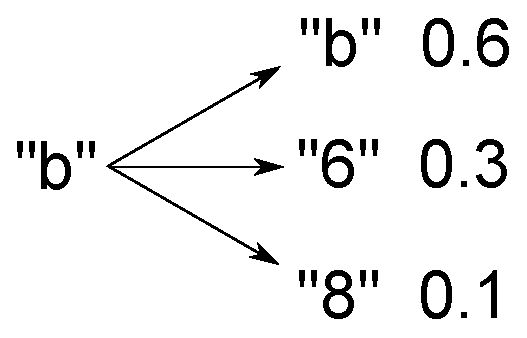
\epsfig{file=figure/correctionStrategy.eps, width=0.3\columnwidth}
\caption{An Simplified Correction Strategy}
\label{fig:corrstrategy}
\end{figure}

\subsubsection{Scoring Policy}
\label{sec:score}
In the fuzzy parser, two scoring policies are designed 
in order to solve fuzzy matching 
problems in content-based data description and spatial information description respectively.

\paragraph{Scoring Policy for Data Description}
Due to the limitations of OCR techniques, data derived from images is not 100\% 
correct. To tolerate the errors and noises in the OCR results, a scoring 
policy is proposed to take consideration of the constraints and OCR results. 

% For primitive expression, a error score is calculated based on the range, 
% length and precision information. 
% \KZ{What is base type expression? It wasn't
% mentioned before. And fix all the back quotes! If it's math expression or
% inline equation, use math mode $..$} 
The calculation of error score $es(e, t)$ derived from the edit 
distance. It uses an expression and a text box content in XML as inputs. 
Specifically, we use the edit distance result as 
the error score for the {\em constant}. 
\begin{equation}
es(c, t) = ed(c, t)
\end{equation}
For the {\em name} of the integer and floating point type, 
edit distances are calculated between the potential data and each number 
which satisfies the range, length or precision information requirements. 
The smallest edit distance is chosen as the error score. 
If $Z$ is the set of all integers and $R'$ is the set of 
all floating points that in length $l$ and precision $p$, 
the error score is calculated as: 
% \begin{multline}
\begin{equation}
es(x(int, a, b), t)=\min\{ed(i, t)| ~~\forall i \in Z, i \in \lbrack a, b \rbrack\}
\end{equation}
% \scalebox{0.8}{ 
% \parbox{1.2\textwidth}{
\begin{equation}
es(x(float, l, p, a, b), t)=\min\{ed(i, t)| ~~\forall i \in R', i \in \lbrack a, b \rbrack\}
\end{equation}
% }}
% \end{multline}
For example, if the expression is {\em constant} ``Vent. rate'' and 
the value is ``Vcnt. rule,''
the error score will be the edit distance between them which is 2. 
If the expression is {\em name} and {\em constraints} $x(int, 60, 100)$ 
and the value is ``53,'' the error score will be 1, since for all integers 
between 60 and 100, one of the minimum edit distances with ``53'' is 
the edit distance of ``63'' and ``53'', which is 1. 

Using error score computation method, we can further compute $esm(e, t, M)$ 
which is the error score with the correction model. We first define $cor(t, S)$, 
which takes a text box content $t$ and a correction strategy $S$ as inputs. 
This function will give us a set of candidate corrected text box contents and 
corresponding probabilities by replacing the substring of $t$ to new candidates 
according to $S$. In $cor(t, S)$, $rep(t, m, n)=t'$ means that $t'$ is the 
result of replacing all occurances of $m$ in the string $t$ with $n$. 
\begin{equation}
cor(t, S)=\{(t',p)|~~\forall (m,n,p) \in S, rep(t,m,n)=t'\}
\end{equation}
Then the error score with correction model $esm(e, t, M)$ will 
find the minimum product of the error score $es(e, t')$ and the probability $p$. 
\begin{equation}
esm(e, t, M)=\min\{es(e, t')*p | ~~\forall S \in M, \forall (t', p) \in cor(t, S)\}
\end{equation}
% In the 
% correction model, a substring of the OCR results is attached with the potentional 
% right results and the probability for it being corrected as the new one. 
% The generation of 
% the correction model will be further explained in \secref{sec:correction}. 
% \KZ{I'm not sure if I understood the following model correctly. C is not 
% properly explained.}
% \begin{figure}
% \begin{equation}
%   \mbox{Correction Strategy:}~ C(oriStr)=newStr
% \end{equation}
% \begin{equation}
%   \mbox{Correction Model:}~ M = \{(C, Prob(C)) ~|~ \forall C\}
% \end{equation} 
% \caption{Incremental Learning Model for Human Correction}
% \label{fig:corrModel}
% \end{figure}

% example
% \begin{algorithm}
% \caption{Error Score Computation Without Correction Model}
% \label{alg:errScore}
% \begin{algorithmic}
% \REQUIRE ~~\\
% The constant or name description $e$ and $data$.
% \ENSURE ~~\\
% The error score $errScore$
% \IF{$e$ is $c$}
% \STATE{$es$ = edit distance of $c$ and $data$}
% \ELSIF{$e$ is $x(int, min, max)$}
% 	\FOR{each integer $i$ between $min$ and $max$}
% 	\STATE{$es$ = the minimum edit distance between $i$ and $data$}
% 	\ENDFOR
% \ELSIF{$e$ is $x(float, l, p, min, max)$}
% 	\FOR{each floating-point $i$ with length l, precision p and between $min$ and $max$}
% 	\STATE{$es$ = the minimum edit distance between $i$ and $data$}
% 	\ENDFOR
% \ENDIF
% \end{algorithmic}
% \end{algorithm}

% \begin{algorithm}
% \caption{Error Score Computation With Correction Model}
% \label{alg:errScoreM}
% \begin{algorithmic}
% \REQUIRE ~~\\
% The constant or name description $e$, $data$ and correction model $m$
% \ENSURE ~~\\
% The error score with correction model $errScoreM$
% \FOR{each potentional correction result $dataCorrected$ of $data$ using $m$}
% \STATE{$errScoreM$ = the minimum product of $es$ between $e$ and $dataCorrected$ and 
% the probability of $data$ being corrected as $dataCorrected$ }
% \ENDFOR
% \end{algorithmic}
% \end{algorithm}

The total score for the description is calculated by adding all the error scores 
together. By adding all the error scores together, we can balance the tolerance for 
errors in a sub expression and the overall sequence. 
% \KZ{I think you can
% give a complete formula for the whole description.} 
% example

\paragraph{Scoring Policy for Spatial Description}
In ODL, spatial description is used to describe the rough spatial 
relationship based on human estimates. In order to minimize human efforts
in estimating the spatial distances, a spatial score $ss(coor, cc)$ 
is used, which measures the differences between the provided spatial 
description and data.
% for handling such 
% description fuzzily is used.  
It takes the coordinates of the text box ($coor$) and the position of the current cursor ($cc$) 
as inputs. 
In the semantics, we record the position 
of the parsing cursor, which is the current location of the parsing process. 
For all potential input data, the spatial score is calculated according 
to the distance between the data coordinates and the cursor. 
% \begin{figure}[ht!]
% \begin{equation*}
\begin{equation}
	ss(cc, coor) = ||cc - coor||
\end{equation}
% \caption{Spatial Score Computation}
% \label{alg:ss}
% \end{equation*}
% \caption{Spatial Score Computation}
% \label{alg:ss}
% \end{figure}

\subsubsection{Evaluation Rules}

In those previous sections, we introduce some methods of processing the input data in order to tolerate some errors in the input data. In this section, we describe the evaluation rule for generating the parser. 
The resulting parser is a list of all candidate parsing trees. Two scoring 
policies are used to relieve the computational cost by filtering low probability results. Those specific rules for parsing are shown in Figure 14 in the form of inductive judgement forms. Those functions defined in Figure 13 would be used in the those inductive rules.
The {\em Cons} function is one of the key functions of parsing. It takes 
the current position of the cursor $c$, a text box $tb$ and the expression $e$ as the input 
and return true or false for whether the text box is a suitable candidate for the 
expression. The function will evaluate the content of the text box based on 
the scoring policy for data description and the spatial position 
with the cursor according to the scoring policy for spatial description. 
A threshold {\em t} is set for the sum of the two scores.
\begin{equation}
Cons(tb, c, e) = 
\begin{cases}
\text{T}& \text{$esm(e, tb.t, M)+k*ss(c, tb.c) < t$}\\
\text{F}& \text{otherwise}
\end{cases}
\label{equ:constraint}
\end{equation}

The {\em Find} function is 
designed for finding all potential results that satisfy the scoring policies. 
The parsing process involves mapping the semi-structured data with the expression. 
{\em Filter} is designed to filter the results based on the various constraints. 
Due to 
the spatial feature of the semi-structured data, 
a variable named {\em c} is used 
in the environment to record the position of the cursor.
In the judgement form that we designed to represent the parsing process, an ODL 
expression, provided with the environment {\em E} and input data {\em D}, will be 
evaluated into a list of parse trees and remaining data {\em D'}.
\[
  {\rm Judgment~ Form:}~~ E,D;e \Downarrow (D';parse\_tree)list
  \label{semantics:judegement} 
\]
% where E is environment, D and D' are input\_data, C records the position of the cursor.

Evaluation rules \ref{rule:x}, \ref{rule:c1} and \ref{rule:c2} are used 
for evaluating variable expression and constant expression respectively. 
For each expression every given text box will be checked and will be 
considered as a potential result if it satisfies the constraints. 
For example, given {\em constant} ``Vent. rate'', current cursor at ``(132, 0)'' and some potential text boxes ``(c=$\langle$264,33, 336,45$\rangle$, t=``Vcnt. rule'')'' and ``(c=$\langle$264,51,439,64$\rangle$, t=``PR Interval'')'', the error score for the first text box is much lower compared to the second one. According to \ref{rule:c1}, the first text box will be considered as a potential result 
for the expression and the second text box will not be a potential result, according to \ref{rule:c2}. For {\em name} and {\em constraints}, filtering based on the constraints will take place after generating all the results for the {\em name}. 

Evaluation rule \ref{rule:coor}, \ref{rule:hskip} and \ref{rule:vskip} 
are used for evaluating spatial operations. \ref{rule:coor} indicates that the data searching area 
will be limited when providing coordinate information. 
For example, in {\em constraints} expression ``e($\langle$0.1w,\_,0.5w,\_$\rangle$)'', ``w'' is short for the 
width of the whole document, which is 1328 pixels and the length of the whole document is 1000 pixels in this case. All the data pairs outside of 
the rectangle, for instance outside the upper left and bottom right corners of which are ``(132, 0)'' and ``(664, 1000)'', will not be considered. 
\ref{rule:hskip} and \ref{rule:vskip} 
indicates the remaining data after skipping. 

For union, \ref{rule:union} indicates that each component 
of the union description will be considered. For example, to parse the 
{\em union} description (``month\_str'') used for the names of the months, 
every possible month name will be tried and they will be filtered 
by the constraints of the union expression and the context. 
% The {\em union} description will be considered 
% The 
% {\em union} description will be considered {\em constant} ``Feb'' and generated corresponding candidate results together with the results when it is considered as the rest names. 

{\em Struct} and {\em list} share 
similar evaluation processes according to \ref{rule:struct} and \ref{rule:list}. These rules say 
that data will be binding to them in sequence. For example, to parse the {\em struct} for ``triple'', the results for ``Vent. rate'' will be generated first, and then results for ``hskip $\backslash$s'' will be generated based on the remaining data after ``Vent. rate'' generation. 

% \subsubsection*{Data Description Expression}
% The evaluation rule for variable description and constant description is described 
% as \ref{rule:x1}, \ref{rule:x2}. The idea is that, based on the 

% \subsection{Example}

\begin{figure}[ht!]
\tiny
\centering
% \begin{eqnarray*}
% \text{text~~box} ::=&&\{c=\text{coor}, t=v\}\\
% &&|\{\}\\
% \text{parse\_tree} ::=&&()\\
% &&|((e,text~~box), [parse\_tree_1,...,parse\_tree_n])\\
% \text{input~~data} ::=&& set ~~ of ~~ text~~boxs\\
% \end{eqnarray*}

\begin{align*}
% \centering
% \[
  Cons:text\_box~*&~coor*expression \rightarrow bool \\
% \]
% \[
  Find:input\_data~*&~coor*value \rightarrow input\_data \\
% \]
\end{align*}
\begin{align*}
% \centering
% \[
  Begin:&~input\_data \rightarrow coor \\
% \]
% \[
  End:&~input\_data \rightarrow coor \\
% \]
\end{align*}
%\vspace{-6 mm}
\[
  Filter:(input\_data*parse\_tree)list*expression \rightarrow (input\_data*parse\_tree)list 
\]
\[
  Hskip:input\_data*coor*(input\_data*parse\_tree)list \rightarrow input\_data 
\]
\[
  Vskip:input\_data*coor*(input\_data*parse\_tree)list \rightarrow input\_data 
\]

\caption{Functions in Semantics}\label{fig:funseman}
\end{figure}

\begin{figure}[ht!]
\tiny
% \[
%   {\rm Judgment~ Form:}~~ E,D;e \Downarrow (D';parse\_tree)list
%   \label{semantic:judegement} 
% \]
% where E is environment, D and D' are input\_data, C records the position of the cursor.
% \begin{minipage}[c]{0.45\textwidth}
\begin{gather*}
  \tag{\sc E-Empty}\label{rule:empty}
  \frac
  {}
  {E,\{\};x \Downarrow []}\\
  % \tag{\sc E-X1}\label{rule:x1}
  % \frac
  % {p \in D ~~ E(c)=coor ~~ Cons(p, coor, type)=true ~~ E,(D-p);x \Downarrow r}
  % {E,D;x \Downarrow (\{\};(x(type), p),[])::r}\\
  % \tag{\sc E-X2}\label{rule:x2}
  % \frac
  % {p \in D ~~ E(c)=coor ~~ Cons(p, coor, type)=false ~~ E,(D-p);x \Downarrow r}
  % {E,D;x \Downarrow (\{p\};(x(type), \{\}),[])::r}\\
  \tag{\sc E-C1}\label{rule:c1}
  \frac
  {p \in D ~~ E(c)=coor ~~ Cons(p, coor, const)=true ~~ E,(D-p);x \Downarrow r}
  {E,D;const \Downarrow ((D-p);(const, p),[])::r}\\
  \tag{\sc E-C2}\label{rule:c2}
  \frac
  {p \in D ~~ E(c)=coor ~~ Cons(p, coor, const)=false ~~ E,(D-p);x \Downarrow r}
  {E,D;const \Downarrow (D;(const, \{\}),[])::r}\\
  \tag{\sc E-X}\label{rule:x}
  \frac
  {p \in D ~~ E(c)=coor ~~ E,(D-p);x \Downarrow r}
  {E,D;x \Downarrow ((D-p);(x, p),[])::r}\\
  % \tag{\sc E-Name}\label{rule:name}
  % \frac
  % {E(x)=v ~~ E(c)=coor ~~ Find(D, c, v)=D'}
  % {E,D;*x \Downarrow \sum_{p_i \in D'}((D'-p_i);(*x, p_i),[])::[]}\\
  \tag{\sc E-Constraint}\label{rule:Constraint}
  \frac
  {E,D;e_0 \Downarrow r_0 ~~~~ \forall i: r_{i+1}=Filter(r_i, e_i)}
  {E,D;e_0(e_1, e_2, ..., e_n) \Downarrow r_{n+1}}\\
  \tag{\sc E-Coor}\label{rule:coor}
  \frac
  {Find(D, coor, nil)=D' ~~ E[c \mapsto Begin(D')],D';e \Downarrow (D'';t)list}
  {E,D;e(coor) \Downarrow (D-D'+D'';t)list}\\
  %\end{gather*}
  %\end{minipage}
  %\hfill \begin{minipage}[c]{0.45\textwidth}
  %\begin{gather*}
  % \frac
  % {E,D;e \downarrow r}
  % {E,D;e~~as~~x \Downarrow }\\
  \tag{\sc E-Hskip}\label{rule:hskip}
  \frac
  {E,D;e \Downarrow r ~~ E(c)=coor ~~ Hskip(D, coor, r)=D'}
  {E,D;hskip~~e \Downarrow (D';[])::[]}\\
  \tag{\sc E-Vskip}\label{rule:vskip}
  \frac
  {E,D;e \Downarrow r ~~ E(c)=coor ~~ Vskip(D, coor, r)=D'}
  {E,D;vskip~~e \Downarrow (D';[])::[]}\\
  \tag{\sc E-Union}\label{rule:union}
  \frac
  {E,D;e_1 \Downarrow r_1 ~~ E,D;\{e_2|..|e_n\} \Downarrow r_2}
  {E,D;\{e_1|e_2|...|e_n\} \Downarrow r_1+r_2}\\
  \tag{\sc E-Sturct}\label{rule:struct}
  \frac
  {E,D;e_1 \Downarrow (E',D';parse\_tree)list~~~~  \forall i:  E'_i[c \mapsto End(D-D_i')],D_i';\{e_2,...,e_n\} \Downarrow r_i}
  {E,D;\{e_1,e_2,...e_n\} \Downarrow \sum_{i=1}^{m} (D';parse\_tree)list*r_i}\\
  \tag{\sc E-List}\label{rule:list}
  \frac
  {E,D;head ~~e~~list \Downarrow (E',D';parse\_tree)list ~~~~ \forall i:  E'_i[c \mapsto End(D-D_i')],D_i';tail~~e~~list \Downarrow r_i}
  {E,D;e~~list \Downarrow \sum_{i=1}^{m} (D';parse\_tree)list*r_i}\\
  % \tag{\sc E-List}\label{rule:list}
  % \frac
  % {E,D;e \Downarrow (E',D';parse\_tree)list ~~~~ }
  % {E,D;e ~~ list \Downarrow }\\
\end{gather*}
%\end{minipage}
\caption{Semantics}\label{fig:semantics}
\end{figure}


% Describe the process of parser generation. 
% \begin{enumerate}
% \item Using inference rules;
% \item How to use the spatial information we have;
% \item How to design the scoring policy to handle the noises and errors.
% \end{enumerate}

% \begin{figure}
% % \centering
% \begin{eqnarray*}
% \text{pair} ::=&&\{c=\text{coor}, t=v\}\\
% &&|\{\}\\
% \text{tree} ::=&&[]\\
% &&|((e,pair), [t_1,...,t_n])\\
% % \text{data} ::=&&pair ~~ list\\
% % \text{report} ::=&&pair\\
% % &&|NF\\
% % &&|pair ~~ list\\
% % \text{map} ::=&&\{e=v, r=report\}\\
% % \text{maps} ::=&&map ~~ list\\
% % \text{result} ::=&&\{\{v_1,pair_1\}, ..., \{v_n,pair_n\}\}\\
% \end{eqnarray*}
% \caption{Data}\label{fig:data}
% \end{figure}

% \begin{figure}
% % \centering
% \begin{eqnarray*}
% % \text{parse}(e, data) ::=&& \text{parse}(v, date)\\
% \text{score}(maps):&& maps->float\\
% % \text{opt}(maps ~~ list):&& maps ~~ list->map~~list\\
% \text{opt}(maps ~~ list):
% &&if ~~ score(head~~(maps~~list))>score(opt(tail~~(maps~~list)))\\
% &&then ~~ head~~(maps~~list)\\
% &&else ~~ opt(tail~~(maps~~list))\\
% \text{limit}(coor, data):
% &&if ~~ (head ~~ data).c \in coor\\
% &&then ~~ (head ~~ data)::limit(coor, tail~~data)\\
% &&else ~~ limit(coor, tail~~data)\\
% \text{used\_data}(maps):
% &&if ~~ (head~~maps).r != NF\\
% &&then ~~ (head~~maps).r::used(tail~~maps)\\
% &&else ~~ used\_data(tail~~maps)\\
% \text{remain\_data}(maps, data):
% &&data-used\_data(maps)\\
% \text{parse}(x, pair):
% &&let ~~ map ~~ = \{e=x, r=pair\}~~in\\
% &&if~~score(map)>threshold\\
% &&then~~map::[]\\
% &&else~~\{e=x, r=NF\}::[]\\
% \text{parse}(x, data):
% &&let ~~ mapslist ~~ = parse(x, head~~data)::parse(x, tail~~data)::[]~~in\\
% &&opt~~(mapslist)\\
% \text{parse}(e=\{e_1 | e_2 | ... | e_n\}, data):
% &&let ~~ mapslist ~~ = parse(first~~e, data)::parse(rest~~e, data)::[]~~in\\
% &&opt~~(mapslist)\\
% % doubt
% \text{parse}(e=\{l_1 = e_1, ..., l_n = e_n\}, data):
% &&let ~~ maps = parse(head~~e, data)~~in\\
% &&maps::parse(tail~~e, remain\_data(maps, data))\\
% % &&if ~~ type((head ~~ e)) ~~ is ~~ record\\
% % &&then ~~ combine(parse(head ~~ e, data), parse(tail~~e, remain_data))\\
% % &&else ~~  
% \text{parse}(e=e_0{_{(coor)}}, data):
% &&let ~~d_{limit} = limit(coor, data)\\
% &&parse(e_0, d_{limit})\\
% \text{parse}(e=e_0 ~~ list, data):
% &&let ~~ maps = parse(head~~e, data)~~in\\
% &&maps::parse(tail~~e, remain\_data(maps, data))\\
% \text{parse}(e.l, data):
% &&let ~~ e_1 = e.l ~~in\\
% &&parse(e_1, data)\\
% \text{parse}(e=hskip ~~ e_1, data):
% &&let ~~ pairlist = \\
% &&if ~~ e_1>0\\
% &&then ~~ (head~~data)::parse(e=hskip~~(e_1-(head~~data).coor.length), tail~~data)\\
% &&else []\\
% &&in ~~ \{e=hskip~~e_1, r=pairlist\}::[]\\
% % \text{parse}(e=vskip ~~ e_1, data):
% % &&let ~~ pairlist = \\
% % &&if ~~ e_1>0\\
% % &&then ~~ \\
% % &&let ~~ remain = \\
% % &&if ~~ 
% % (head~~data)::parse()
% % &&\text{parse}(e_{(coor)}, data)=\\
% % &&~~d_{limit} = \{p | p \in data.i, ~~ p.coor \in coor \}\\
% % &&~~\text{parse}(e, d_{limit})\\
% % &&\text{parse}(v, line)=\\
% % &&~~results ~~ = cons[result] ~~ nil[result] ~~ \text{parse}(v, head[pair] ~~ line)\\
% % &&~~results ~~ = cons[result] ~~ results ~~ \text{parse}(v, tail[pair] ~~ line)\\
% % &&~~return ~~ opt(results)\\
% % &&~~for ~~ pair ~~ in ~~ line:\\
% % &&~~~~results ~~ add ~~ (v, pair)\\
% % &&~~return ~~ opt(results)\\
% % &&\text{parse}(v, data)=\\
% % &&~~for ~~ line ~~ in ~~ data:\\
% % &&~~~~results ~~ add ~~ \text{parse}(v, line)\\
% % &&~~return ~~ opt(results)\\
% \end{eqnarray*}
% \caption{Semantic}\label{fig:semantic}
% \end{figure}

% \begin{figure}[ht!]
% \centering
% \begin{equation}
%  generate:expresion*data \rightarrow \{parse\_tree, remain\_input\} ~~ list
% \end{equation}
% \begin{equation}
%   score:parse\_tree \rightarrow float
% \end{equation}
% \begin{eqnarray*}
%   \lefteqn{generate(x, pair::data)=}\\
%   &&let \\
%   &&~~ tree = leafnode(\{x, pair\})\\
%   &&in\\
%   &&~~ \{tree, data\}::generate(x, data)\\
%   \lefteqn{generate(e=\{e_1 | e_2 | ... | e_n\}, pair::data)=}\\
%   &&append ( generate(e_1, pair::data) , generate(\{e_2|...|e_n\}, pair::data))\\
%   \lefteqn{generate(e=\{l_1 = e_1, ..., l_n = e_n\}, pair::data)=}\\
%   &&let\\ 
%   &&~~ combine(tree_1, \{tree_2, ri\}::remainlist) = \\
%   &&~~~~ \{(tree_1;tree_2), ri\}::combine(tree_1, remainlist)\\ 
%   &&~~ help(\{pt, ri\}::results) = \\
%   &&~~~~ append (combine(pt, (generate(tail ~~ e, ri))), help(results))\\
%   &&in\\
%   &&~~ help(generate(head ~~ e, pair::data))\\
%   \lefteqn{generate(e = e_0 ~~ list, pair::data)=}\\
%   &&let\\ 
%   &&~~ combine(tree_1, \{tree_2, ri\}::remainlist) = \\
%   &&~~~~ \{(tree_1;tree_2), ri\}::combine(tree_1, remainlist)\\ 
%   &&~~ help(\{pt, ri\}::results) = \\
%   &&~~~~ append (combine(pt, (generate(tail ~~ e, ri))), help(results))\\
%   &&in\\
%   &&~~ help(generate(head ~~ e, pair::data))\\
%   \lefteqn{generate(e=e_0{_{(coor)}}, pair::data)=}\\
%   &&let\\
%   &&~~ limit(coor, pair::data) = \\
%   &&~~~~ if ~~ pair.c \in coor\\
%   &&~~~~ then ~~ \{pair::limit(coor, data).1, limit(coor, data).2\}\\
%   &&~~~~ else ~~ if ~~ pair.c ~~ after ~~ coor\\
%   &&~~~~ then ~~ \{limit(coor, data).1, pair::limit(coor, data).2\}\\
%   &&~~~~ else ~~ \{limit(coor, data).1, limit(coor, data).2\}\\
%   &&~~ data_{limit} = limit(coor, pair::data).1\\
%   &&~~ data_{remain} = limit(coor, pair::data).2\\
%   &&~~ combine(data_{re}, \{tree, ri\}::results) = \\
%   &&~~~~ \{tree, data_{re}::ri\}::combine(data_{re}, results) \\
%   &&in\\
%   &&~~ combine(data_{remain}, generate(e_0, data_{limit}))\\
%   \lefteqn{generate(e.l, data)=}\\
%   &&let\\
%   &&~~ e_1 = e.l\\
%   &&in\\
%   &&~~ generate(e_1, data)\\
%   \lefteqn{generate(e=(hskip e_0), pair::data)=}\\
%   &&if ~~ e_0 > 0 ~~ and ~~ pair != newline\\
%   &&then ~~ combine(leafnode{pair}, generate(hskip (e_0-pair.length), data))\\
%   &&else ~~ []\\
%   \lefteqn{generate(e=(vskip e_0), data)=}\\
%   &&if ~~ e_0 > 0 ~~ and ~~ pair == newline \\
%   &&then ~~ combine(leafnode{pair}, generate(vskip (e_0-pair.height), data))\\
%   &&else ~~ if ~~ pair != newline\\
%   &&then ~~ combine(leafnode{pair}, generate(vskip e_0, data))\\
%   &&else ~~ []\\
% \end{eqnarray*}
% \caption{Semantic}\label{fig:semantic}
% \end{figure}

% \subsection{Human Correction}
\label{sec:correction}
The parse tree returned from the previous process may contain errors. 
Our system prompts the user to manually correct some of these errors
and such rectification goes into the correction model which improves the
overall accuracy.
% \item incremental learning model, features;
% \item How do we figure out which error should be corrected first;
% \item What will happen after an error been corrected and 
% why the process is incremental.

\subsubsection{Incremental Learning Model}
\label{sec:incremental}
The correction model mentioned in \secref{sec:corrmodel} 
is an incremental learning model. 
%The reason for this is that the model is incrementally changed 
%according to the corrections that humans make. 
The design of the correction model adheres to the scoring
policy in \secref{sec:score}.

\paragraph{Initial Model}
% \KZ{Correct all the backquotes!}
The initial model without any human correction
is generated using the candidate results of the OCR 
engine. For example, for ``QRS'' in the example image, based on the OCR 
engine, the most reliable result is ``ORS''. Other top candidates are 
``QPS'', ``QRS'' and ``OPS''. Thus the system learns that ``OR'' may
be corrected as ``QP'', ``QR'' or ``OP''. These three candidates 
will be added into the initial model. 

To calculate the probabilities of the correction candidates in the initial 
model, we count the occurrences of each correction. In the example, the 
probabilities for ``OR'' corrected as ``OR'', ``QP'', ``QR'' 
or ``OP'' are equal since such corrections only happened once. 

% \[
% P(newStr|oriStr) = \frac{occurrence ~of~ ()}{\sum_{tar \in all} occurrence ~of~ C(oriStr)=tar}
% \]

\paragraph{Training From Human Correction}
After generating the parsing results using the initial model, we have 
made full use of the OCR engine. To correct the remaining errors, 
human input is applied. 
%The incremental learning model is also suitable 
%for learning from human correction. 
For example, if a human corrects the error result ``1o.o'' to ``10.0'', 
we can learn from it ``o''s in the OCR results could have been
``0''s. Thus the correction strategy 
for ``o'' is modified and ``0" is the new correct candidate. 
We also calculate the occurrence 
of different human correction for the probability calculation. 

\paragraph{Application of the Model}
The model for correction is used in the scoring policy in the 
fuzzy parser. As shown in \secref{sec:score}, for each 
description, our system will consider all the potential  
results based on the correction strategies in the model. 
For the description ``QRS'' and the most confident results 
``ORS'', we try all the strategies in the model 
and consider both whether the corrected result satisfies the 
description and whether the correction strategy is 
feasible. In this example, since the four correction strategies 
have the same probability, we choose ``QR'' as the correction 
result for ``OR'', 
which has the lowest error score based on the description.  

\subsubsection{Manual Correction Policy}
In this section, we describe the policies for recommending 
errors to be manual corrected. When making use of human correction, 
some of errors have a greater impact on 
accuracy if they are corrected. The reason is some similar errors 
occur frequently. Which errors are recommended to a user 
for correction will affect the accuracy and the 
number of corrections that the user has to made. 

\paragraph{Random}
The baseline for correction recommendation is random 
recommendation. Based on the parsing results, we can randomly 
recommend the errors we found for humans to correct.  

% \subsubsection*{Most Frequently Error Type}

\paragraph{Most Frequent Error Description Elements}
Another more effective correction strategy is to 
recommend the description 
elements that contain the most frequent errors. For a set of images 
in similar formats and the corresponding ODL descriptions, 
we discovery which elements in the description are more likely 
to be parsed with errors. For those elements, similar errors 
are more likely to happen since the descriptions for them are the 
same. Consequently, such recommendations are more effective
than a random recommendation. 

% \end{enumerate}

%
\section{Experiment}
In this section, we experiment on different NLG tasks. We first present the experimental setup on different tasks. Then, we show the quantitative and qualitative results together with comprehensive analysis and ablation studies.

\subsection{Implementation Details}
We evaluate the newly proposed ICL strategy on five commonly-researched natural language generation tasks: reading comprehension, dialogue summarization, style transfer, question generation and news summarization. Details on the task description, the strong baseline, corresponding  dataset, evaluation metrics and key hyper-parameters for each task are presented as follows.

\begin{table*}[th]
	\scriptsize
	\centering
	\begin{tabular}{lp{1.1cm}rrrcccc}
		\hline
		Task & Dataset & \#Train & \#Val & \#Test & Input & Output & Avg & Std\\
		\hline
		Reading Comprehension & DREAM & 6,116 & 2,040 & 2,041 & ``Q:''+ question + dialogue & answer & 5.59 & 2.61\\
		Dialogue Summarization & SAMSum & 14,732 & 818 & 819 & dialogue & summary  & 24.99 & 13.06\\
		Style Transfer & Shakespeare & 36,790 & 2,436 & 2,924 & original/modern  & modern/original  & 11.63 & 8.19 \\
		Question Generation & SQuAD1.1 & 75,722 & 10,570 & 11,877 & passage + [SEP] + answer & question & 13.09 & 4.27 \\
		News Summarization & CNNDM & 287,227& 13,368& 11,490 & document & summary & 70.97 & 29.59\\ 
		\hline
	\end{tabular}
	\caption{A summary of tasks and datasets. \#Train, \#Val and \#Test refers to the number of samples in the corresponding dataset. Avg and Std are the statistics for the number of output tokens. ``+'' refers to the concatenation operation.}
	\label{tab:taskdata}
\end{table*}

\textbf{Reading comprehension} is the task that answering questions about a piece of text. We use the DREAM dataset~\cite{sun2019dream} where questions are about corresponding dialogues and the answer is a complete sentence in natural language. We neglect the negative choices in the original dataset and formulate it as a NLG task. We adopt the pre-trained language model BART~\cite{lewis2020bart} as the baseline, where the input is a concatenation of a question and the corresponding dialogue made up of speakers and utterances. 
We experiment with  transformers\footnote{\url{https://github.com/huggingface/transformers}} based on the publically available ``facebook/bart-large'' checkpoint \footnote{\url{https://huggingface.co/facebook/bart-large}}.
%The preceding BART model is also adopted as the baseline, whereas the input is a concatenation of question and a dialogue.
The generated answers are evaluated by BLEU scores\footnote{The BLEU-1/2/3/4 scores are computed according the Google's implementation(\url{https://github.com/tensorflow/nmt/blob/master/nmt/scripts/bleu.py}).}~\cite{papineni2002bleu} widely used for QA systems, together with Meteor and Rouge-L F1 as mentioned above. The parameters are also the same as dialogue summarization, except that the early-stop is activated if there is no improvement on the perplexity of the validation set. 


\textbf{Dialogue summarization} is to generate a concise summary covering the salient information in the input dialogue. The preceding model BART has shown to be a strong baseline for this task, where only the dialogue is concatenated into a single sequence as the input. We experiment with  %transformers\footnote{\url{https://github.com/huggingface/transformers}} based on the publically available ``facebook/bart-large'' checkpoint \footnote{\url{https://huggingface.co/facebook/bart-large}} and 
SAMSum dataset\footnote{\url{https://arxiv.org/src/1911.12237v2/anc/corpus.7z}}~\cite{gliwa2019samsum} for daily-chat dialogues. 
The generated summaries are evaluated by comparing with the reference through evaluation metrics, including Rouge-1/2/L F1 scores\footnote{\url{https://github.com/pltrdy/files2rouge}}~\cite{lin2004rouge}, Meteor~\cite{banerjee2005meteor} and BertScore F1\footnote{Both Meteor and BertScore are calculated by SummEval(\url{https://github.com/Yale-LILY/SummEval}), and the latter one is based on the default bert-base-uncased model.}. We evaluate the model on the validation set after each training epoch and the early-stop patience will be added 1 if there is no improvement according to the Rouge-2 F1 score. The training process terminates when the early-stop patience equals or is larger than 3.  During the inference, the minimum and maximum output length is set to 5 and 100 respectively, with no\_repeat\_ngram\_size=3, length\_penalty=1.0 and num\_beams=4.


% The answer is either a span of words in the original text or a complete sentence in natural language.
\textbf{Style transfer} preserves the semantic meaning of a given sentence while modifies it's style, such as positive to negative, formal to informal, etc.
We adopt the Shakespeare author imitation dataset~\cite{xu2012paraphrasing}, containing William Shakespeare's original plays and corresponding modernized versions. Krishna el al.~\shortcite{krishna2020reformulating} proposed to do unsupervised style transfer by training paraphrase models based on the GPT-2 language model~\cite{radford2019language}. We re-implemented their approach STRAT\footnote{\url{https://github.com/martiansideofthemoon/style-transfer-paraphrase}} and evaluated with the provided script. Evaluation metrics includes 
transfer accuracy(ACC), semantic similarity(SIM), Fluency(FL) and two aggregation metrics, i.e., geometric averaging(GM) and their newly introduced $J(\cdot)$ metric. The hyper-parameter $hp$ equaling 0.0, 0.6 or 0.9  in Table~\ref{tab:end2endst} is the sampling parameter for trades off between ACC and SIM in their approach. 
In the training stage, we evaluate the model after updating every 500 steps. The perplexity on the validation set is used to activate the early-stop which equals 3. The inference is done as default.
 
\textbf{Question generation}~\cite{zhou2017neural} aims at generating a question given an input document and its corresponding answer span. SQuAD 1.1~\cite{rajpurkar2016squad} is generally used for evaluation. We adopt the data split as in \cite{du2017learning} and fine-tune the pre-trained UniLM~\cite{dong2019unified} as the strong baseline according to their official implementation\footnote{\url{https://github.com/microsoft/unilm/tree/master/unilm-v1}}. Generated questions are evaluated by metrics including BLEU-1/2/3/4, Meteor and Rouge-L with the provided scripts. The model is evaluated every 1000 steps and the early-stop equaling 3 is associated with the perplexity on the validation set. Other parameters are unchanged following the official guideline.

\textbf{News summarization} differs from dialogue summarization where the input is a document instead of a dialogue. We adopt the same strong baseline BART and evaluation metrics as dialogue summarization. Experiments are done with CNNDM dataset~\cite{HermannKGEKSB15} consisting of news articles and multi-sentence summaries\footnote{\url{https://github.com/pytorch/fairseq/blob/main/examples/bart/README.summarization.md}}. The model is evaluated every 2000 steps and the early-stop equaling 3 is associated with the Rouge-2 on the validation set. During the inference, the minimum and maximum output length is set to 45 and 140 respectively, with no\_repeat\_ngram\_size=3, length\_penalty=2.0 and num\_beams=4.
%\footnote{Inference parameters are borrowed from \url{https://github.com/pytorch/fairseq/blob/main/examples/bart/summarize.py}}

The summary of each task is listed in Table~\ref{tab:taskdata}. For fair comparisons, we re-implemented baselines following the above instructions on our machine. On top of the above baselines, we further arm them with the ICL strategy according to the Algorithm~\ref{alg:picl}. The settings of newly introduce Start and Stride are specified and discussed in following sub-sections. All of our experiments are done on a single RTX 3090 or a single RTX 2080Ti with 24G and 11G GPU memory respectively.
%and the result are averaged over three runs.


 
\subsection{Automatic Evaluations on Different Tasks}
\label{sec:taskperformances}

We compare our approach with the vanilla models mentioned above and the approach from~\citet{liang-etal-2021-token-wise} as baselines.
The performances on different NLG tasks are shown in Table~\ref{tab:end2end}. 
These tasks not only focus on solving different problems, but also has various amount of training data as well
as reference output lengths as shown
Table~\ref{tab:taskdata}.
Besides, the basic model are also different, including BART, GPT-2 and UniLM. 
Our new training strategy achieves significantly improvements among different tasks on most evaluation metrics, which shows that our method not only works well, but also has strong generalization abilities.

We explain the some specific results as follows:

(1) Our training strategy boosts the performances of the original STRAT with different $hp$ in the style transfer task. GM and J are two comprehensive evaluation metrics, with our approach topping the ranks with significant improvements.

(2) TCL generally performs poorly on tasks
with more training data. For example, it failed on question generation without any improvements over the vanilla model under the same parameter setting, while ICL still 
logs gains. This is mainly due to two reasons.
First, because the nature of TCL is data augmentation which is more effective in low-resource settings,
when training data is abundant, it becomes less useful. 
Second, the way they calculate the loss as sub-sequence generation better suites paraphrasing tasks, such as machine translation tested in their paper, as the order of 
the corresponding tokens between input and output 
are almost the same. Learning such forward mapping can 
be regarded as a kind of ``easy-to-hard'' 
in these limited scenarios.
However, this doesn't hold true for other tasks, 
such as summarization and question generation. 
Therefore, we didn't further test it on CNNDM since
CNNDM has the large amount of training data among
the five.

(3) For news summarization, Rouge-1 scores (precision, recall) for the baseline and our method on CNNDM are (38.16, 52.72) and (40.84, 49.23) correspondingly. Our method made substantial improvements on the precision with a compromise on the recall. 
The meteor score based on the unigram precision and recall emphasizes more on the recall than the Rouge-1 F1. As a result, it drops while Rouge-1 F1 increases. Overall, our method still outperforms BART on this task, especially on F1 scores of Rouge-2 and Rouge-L.




\begin{table}[th]
	\small
	\centering
	\begin{subtable}{\linewidth}
		\scriptsize
		\centering
		\begin{tabular}{lcccccc}
			\hline
			{Method} & {B1} & {B2} & {B3} & {B4} & {Met} & {RL}\\
			\hline
			w/o CL &  32.03 & 16.01 & 8.77 & \textbf{4.80} & 19.84 & 38.89\\
			TCL & 32.53 & 16.25 & 8.52 &4.67 &19.88 & 39.65 \\
			ICL &  \underline{\textbf{33.99}} & \underline{\textbf{17.43}} & \underline{\textbf{9.18 }}& 4.64 & \textbf{20.60} & \textbf{40.78}\\

			\hline
		\end{tabular}
		\caption{Reading Comprehension}
		\label{tab:end2endrc}
	\end{subtable}
	\\[5pt]
	\begin{subtable}{\linewidth}
		\scriptsize
		\centering
		\begin{tabular}{lccccc}
			\hline
			{Method} & {R1} & {R2} & {RL} & {Met} & {BertS} \\
			\hline
			%BART & 52.60&27.00 &42.10 &- & - \\
			w/o CL & 51.88 & 27.30 & 42.77 & 24.75 & 71.38 \\
			TCL  & 52.33 & 27.80 & \textbf{43.91} & 24.59 & 71.77 \\
			ICL & \underline{\textbf{53.07}} & \underline{\textbf{28.23}} & {43.83} & \underline{\textbf{26.12}}& \underline{\textbf{72.17}} \\
			
			\hline
		\end{tabular}
		\caption{Dialogue Summarization}
		\label{tab:end2endds}
	\end{subtable}
	\\[5pt]
	\begin{subtable}{\linewidth}
		\scriptsize
		\centering
		\begin{tabular}{lcccccc}
			
			\hline
			{Method}&$hp$ &  {ACC} & {SIM} & {FL} & {GM} & {J}\\
			\hline
			%\multirow{3}{*}{STRAT}& 0.0 & 71.70 & \textbf{56.40} & 85.20 & 70.10 & 34.70 \\
			%& 0.6 & 75.70 & 53.70 & 82.70 & 69.50 & 33.50 \\
			%& 0.9 & 79.80 & 47.60 & 71.70 & 64.80 & 27.50 \\
			%\hline
			\multirow{3}{*}{w/o CL}& 0.0 & 70.49 & 55.70 & 85.98 & 69.63& 33.72 \\
			& 0.6 &75.31 & 53.46 & 82.56 & 69.27& 33.30\\
			& 0.9 & 78.76 & 47.38 & 74.42 &65.24 & 27.88\\
						\hline
			\multirow{3}{*}{TCL } & 0.0 & 70.31 & \textbf{55.95} &\textbf{87.24} &  70.01& 34.71 \\
			& 0.6 & 74.79 & 53.14 & 82.56 & 68.97 & 33.21 \\
			& 0.9 & 79.41 & 46.88 & 71.92 &64.45 & 26.92 \\
			\hline
			\multirow{3}{*}{ICL}& 0.0 & \underline{73.72} & 55.91 & 86.30 & \underline{\textbf{70.60}} &\underline{\textbf{35.81}}\\
			& 0.6 & 77.26 & \underline{53.80} & \underline{83.87} & \underline{70.38} & 34.64\\
			& 0.9 & \textbf{79.65} & 48.16 & 76.06 & 66.32 & 29.03\\

			\hline
		\end{tabular}
		\caption{Style Transfer.}
		\label{tab:end2endst}
	\end{subtable}
	\\[5pt]
	\begin{subtable}{\linewidth}
		\scriptsize
		\centering
		\begin{tabular}{lcccccc}
			\hline
			{Method} & {B1} & {B2} & {B3} & {B4} & {Met} & {RL}\\
			\hline
			w/o CL & \textbf{50.38} & 35.67 & 27.24 & 21.36 & 24.40 & 50.67 \\
			TCL &\textbf{50.38} & 35.67 & 27.24 & 21.36 & 24.40 & 50.67\\
			ICL &  50.18 & \textbf{35.72} & \textbf{27.36} & \textbf{21.54} & \textbf{24.57} & \underline{\textbf{51.09}} \\
			\hline
		\end{tabular}
		\caption{Question Generation}
		\label{tab:end2endqg}
	\end{subtable}
		\\[5pt]
	\begin{subtable}{\linewidth}
		\scriptsize
		\centering
		\begin{tabular}{lccccc}
			\hline
			{Method} & {R1} & {R2} & {RL} & {Met} & {BertS}\\
			\hline
			%BART &  \\
			w/o CL &  43.07 & 20.01 & 35.94 & \textbf{21.44} & 63.72 \\
			TCL & - & -&- &- &- \\
			ICL & \textbf{43.39} & \underline{\textbf{20.55}} & \underline{\textbf{36.63}} & 19.68 & \textbf{64.05}\\
			\hline
		\end{tabular}
		\caption{News Summarization}
		\label{tab:end2endns}
	\end{subtable}
	\caption{Performances on different NLG tasks. ICL represents the models trained with our ICL algorithm. TCL refers to the previous work from~\cite{liang-etal-2021-token-wise}. Scores underlined are statistically significantly better than both re-implemented baselines with $p<0.05$ according to t-test. }	
	\label{tab:end2end}
\end{table}


\subsection{Human Evaluations}

To further prove the improvement of ICL, we hired three proficient English speakers for human evaluation. 20 samples from the test set of each task are randomly selected, ignoring the ones with totally same generations among three models, including the vanilla model, TCL and ICL. The original input, reference output and three generations are shown to annotators together, while the order of three generations are unknown and different among samples. 3-point Likert Scale is adopted for scoring for each generation~\cite{gliwa2019samsum}, where [1, 3, 5] represent 
excellent, moderate and disappointing results 
respectively. The average scores and agreements 
among the annotators are shown in 
Table~\ref{tab:humaneval}.

The Fleiss Kappa on the first four tasks indicates the fair to moderate agreements. It shows the promising improvement of ICL over the vanilla model and TCL especially on DREAM, SAMSum, and SQuAD1.1, which is consistent with the conclusion based on automatic metrics.
Although the agreement on style transfer is fair, 
our annotators without Shakespeare background 
tend to give low scores to all outputs.
Therefore, the absolute improvement is 
only $0.04$ compared to both baselines.
%This mainly due to the indistinguishable styles between
%Shakespeare’s plays with are quite different from modern languages. 
Besides, the poor agreement on CNNDM reflects the 
diverse concerns of summarization from different 
annotators. Without more specific instructions, they 
tends to focus more on the content coverage instead 
of checking the detailed facts. This is also 
consistent with the higher Meteor scores of the 
vanilla model over ICL.

\begin{table}[th]
	\scriptsize
	\centering
	\begin{tabular}{l|ccc|c}
		\hline
		{Datasets} & {w/o CL} & {TCL} & {ICL} & {Agreement}  \\
		\hline
		DREAM  &3.07 & 2.50&3.20 &0.48 \\
		SAMSum &2.97 &3.57 &3.97 &0.40 \\
		Shakespeare &2.23 &2.23 & 2.27&0.32 \\
		SQuAD1.1 &3.43 & 3.43 &3.77 &0.35 \\
		CNNDM & 3.45 &- &3.40 &0.11 \\
	%	\hline
	%	overall & & & &\\
		\hline
	\end{tabular}
	\caption{Human evaluations. The agreement is calculated by Fleiss Kappa.}
	\label{tab:humaneval}
\end{table}




%Following Liu et al.\shortcite{liu2021competence}'s work, we asked annotators to comparing the performance between our generated results and baselines by choosing from ``Better, Tie, Worse''. 
%The counts for each choice are shown in Table~\cite{}, where the Fleiss Kappa among annotators is ??.

%Analysis





%\subsection{Analysis on Variable Generation Lengths}

%Teacher forcing, which predicts each token given the reference summary tokens during training and given the previous generated tokens during inference, leads to the exposure bias problem for NLG tasks.
%Since ICL starts the training process by predicting the last few tokens of outputs and gradually calculates the loss based on more tokens when the model is stronger, we hypothesis that it can alleviate the exposure bias for training Seq2Seq models to some extent.
%As stated in~\cite{pang2020text}, the output quality tends to degrade as the output length increase with the exposure bias.
%So, we divided the test set of each task according to the length of the generated output into 4 buckets and randomly picked 20 samples in each buckets for both the corresponding baselines and our approach. Each generation is annotated by 5 point Likert Scale, where 1 is the worst and 5 is the best. 

%The trends of performances on variable generation lengths are in Figure~\ref{}.


% \section{Discussion}
\label{sec:discuss}
In this section, we will discuss some implementation details
and the limitations of our system. 
The medical images that we have can pose various problems 
for a traditional OCR engine to process. For example, 
the textual information on the medical images may be 
covered by grid lines as shown in \figref{fig:ecgexample2} or 
in the inverted colour. In these situations, the results of 
the OCR engine will garbled. We preprocess the 
images to remove those noises. First, we threshold the 
images and turn them into binary images. 
% Thresholding is the simplest method of image segmentation. 
Separate thresholds for each of the RGB channels of the image 
are used and combined them with an AND operation. 
In order to automatically threshold the images, 
we make use of ImageJ \cite{schneider2012671}, which implements many
existing auto-thresholding algorithms. 
Then we invert the color of the images if the text 
is white color. 
After preprocessing, we get a simplified version of the 
images and make the text on the images stand out. 
% contrast the text on the images. 
%An example of this preprocessing result is shown in \figref{fig:preprocess}. 

%\begin{figure*}[ht]
%\centering
%\subfloat[Before Preprocessing]{
%\label{fig:preprocess:1}
%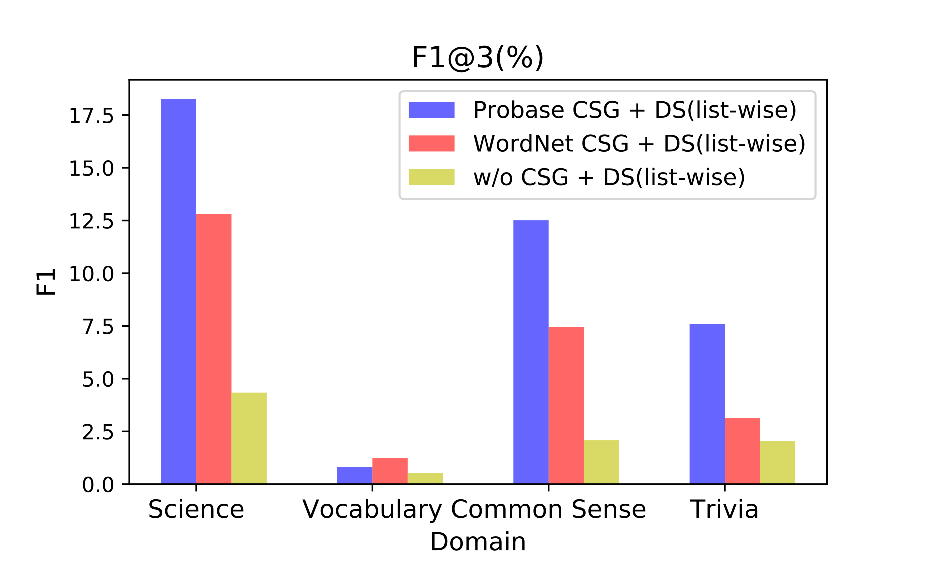
\epsfig{file=figure/f1.eps, width=0.45\columnwidth}
%}
%\hfill
%\subfloat[After Preprocessing]{
%\label{fig:preprocess:2}
%\epsfig{file=figure/pref1.eps, width=0.45\columnwidth}
%}
%\caption{Results of Preprocessing}
%\label{fig:preprocess}
%\end{figure*}
%% \KZ{There seems to be some repetition from the eval section.} 
%

In our system, two parameters are important for the 
performance. 
One is the parameter $k$ in the {\em Constraint} function 
\equref{equ:constraint}, which affects the weight of 
the spatial constraints.
Another is the threshold $t$ in the same function, which 
determines whether the input data satisfy the 
type and spatial constraints based on our scoring policies 
and how many candidates will be generated.  

%\JL{In our system, two parameters which should be defined by ourselves are very important.One is the parameter $k$ in the {\em Constraint} function 
%	\equref{equ:constraint}, 
%	which affects the weight of 
%	the spatial constraints in the whole set of constraints. Another is the threshold we set since an appropriate threshold could give us appropriate numbers of candidates after the selection by filtering some bad results.}
% \KZ{Which param in constraint. The constraint function needs to be
% defined carefully.}
In the implementation process, 
we hold out 20 images separately to train these two parameters 
and choose the ones that have the best performance. 
% some more results

Although our system achieves good results based on our 
experiments, there are some limitations that call for future 
work. First, in order to fuzzy match the information onto the images, 
we need to provide enough constraints in the description, 
such as the type of the 
data or the range of the data. If the constraints are not 
sufficiently specified, it is hard for our system to evaluate what 
data among the OCR outputs are more suitable for the description. 
For example, if we constrain the data to be an integer in the 
description, then any integers that appear in the OCR output can be 
candidates if they satisfy the spatial constraints. 
In many cases, insufficiency in the constraints can be 
made up by the constraints indicated from the neighboring descriptions. 
But sometimes, simple descriptions will lead to sub-standard results. 
Second, the correction model 
we generated is a probabilistic model based on the statistics. 
This correction model can make mistakes, 
e.g., correcting the right answer into the wrong one. More data 
from manual correction will help to reduce this possibility. 

% \KZ{Perhaps there's more issues you can discuss, now that u have
% changed the def of the correction model...}


\section{Related Work}
This section surveys previous works on question generation and tree encoding
respectively.

Text question generation has attracted the attention 
after the work of ~\citeauthor{du2017learning}~\shortcite{du2017learning}, who uses deep seq2seq model 
to generate questions from a raw text paragraph. 
Before that, text question generation relied heavily on hand-craft 
question patterns~\cite{HeilmanS10,LabutovBV15,MostowC09} which is time and 
labor consuming. 

However, this pure seq2seq model is not focused and 
has no control over part in the paragraph to generate question. 
~\citeauthor{zhou2017neural}~\shortcite{zhou2017neural} proposed to encode 
key phrase information using binary indicators to generate 
key-aware questions and they assumes the answer to be key phrase. 
Considering key phrase (answer) is unavailable in reality, 
~\citeauthor{SubramanianWYT17}~\shortcite{SubramanianWYT17} applied 
a two-stage approach. First, key phrases are extracted by 
pointer network~\cite{ptrnet}. Second, 
key phrases are encoded in the same way as 
Zhou et al. With the intuition that questions could be asked in many ways, 
~\citeauthor{Yao2018vae}~\shortcite{Yao2018vae} used conditional-VAE to 
increase the diversity of questions. More recently, models with 
auxiliary feature information~\cite{HarrisonW18} helped improve 
the question quality. Structure question generation aims at 
converting structured data such as triples in knowledge graph to questions. 
~\citeauthor{SerbanGGACCB16}~\shortcite{SerbanGGACCB16} proposed a model to generate factoid questions from knowledge base triples.  None of the above work
considered using parse tree structures to aid question generation process,
which is the focus of this paper.

Sequential RNN model takes sentence as a sequence of words, 
ignoring the syntactic information. In order to utilize
such syntactic information with sequential information, 
~\citeauthor{tai2015improved}~\shortcite{tai2015improved} proposed Tree-LSTM to 
encode the binary parse tree recursively in a bottom-up fashion to 
classify sentiment. In text generation task, 
\citeauthor{eriguchi2016tree}~\shortcite{eriguchi2016tree} 
proposed a tree-to-sequence model with attention mechanism to do 
machine translation and 
~\citeauthor{liang2018automatic}~\shortcite{liang2018automatic} proposed a 
tree-to-sequence model which could handle arbitrary trees, 
to do code comment generation. Our work is inspired by these previous
attempts and we are first to adapt structure encoded neural models to
textual question generations.
\section{Conclusion}
We implement a novel sequence-based dependency parsing
framework which takes advantage of high order features 
in parsing history. 
%We can also adapt beam search to this framework so as to
%relax the strictly greedy nature. Vine pruning\cite{rush2012vine} could
%be incorporated to speed up the parsing.
More importantly, we discovered that the parsing accuracy is very sensitive to
the quality of parsing sequence. Future work can be focused on
developing better sequence predictors that outperform Malt action classifier.
Furthermore, we use two sets of features for sequence predictor and
head mapper right now. A unified set of features between these two components
are worth exploring.
%Besides, better sequence predicting method and unified feature
%representation of two components are worth exploring.
%
%Though we currently get a not bad result,
%the sequence predictor still needs more exploration.
%According to our experiment, slightly changes
%on the sequence can lead to a fatal decline on accuracy. Ensuring the match degree of training sequence and testing
%sequence demands a high quality of sequence predictor.
%
%Further, the features in our current implementation are not expanded and well tuned yet  and we are free to define high order features to make use of parsing history. Our framework is flexible to merge other technics to enhance the performance. Introducing beam could make up for our greedy decoder and improve our accuracy. Vine pruning\cite{rush2012vine} could speed up parsing process. Besides, better sequence predicting method and unified feature representation of two components are worth exploring.


% \IEEEraisesectionheading{
% % \section{Introduction}

Protein$-$protein interactions (PPIs) are of central importance for the majority of biological functions, such as signal transduction, metabolic pathways, molecular dynamics, and protein networks\cite{Hoffmann.Krallinger.ea:2005}, for they serve as the most fundamental building blocks of the entire interacademic systems of any organisms. Collecting data on pairwise interaction relationships is essential for multiple purpose, including identification of modules with certain functionality\cite{Spirin.Mirny.03}, mapping diseases to dominated genes\cite{Ideker.Sharan.08}, and after all, understanding wholistic metabolic/genetic networks from a system biology perspective.

A lot of databases have been built to store protein and genetic interactions from major model organism species and are available in various standardized formats, such as MINT\cite{Zanzoni.Montecchi-Palazzi.ea:2002}, BIND\cite{Bader.ea:2003}, BIOGRID\cite{DBLP:journals/nar/StarkBRBBT06}, etc. Among those mainstream databases, the data largely rely on voluntary reports by scientists or researchers, besides, comprehensive curation efforts become indispensable for the sake of accuracy. However, the amount of biology-related literatures with respect to protein interactions grows explosively and thus make it either impossible or impractical to manually detect PPI information anymore.

Considering huge amount of PPI information with great wealth hidden in published papers, in recent years, numerous mining techniques have been proposed that aim to extract PPI information automatically from free text, especially machine learning, information retrieval, and natural language processing\cite{DBLP:journals/bib/WinnenburgWPDS08}.These approaches can be roughly categorized into three classes: co$-$occurrence, rule$-$based, and machine learning. 

Co$-$occurrence is the approach with most simplicity and naivete. Just as its name implies, this method intends to find out pairs of proteins that co-occur in the same context. The scope of "same context" ranges from phrase, sentence, paragraph to whole abstract, even document. The underlying assumption is that whenever two proteins are mentioned together by authors, chances are high that there is some kind of relationship between them. However, however, in-context closeness even semantic relation does not necessarily represent actual biological interaction. As a consequence, a large fraction of candidate pairs are mismatched inevitably, causing a high recall but low precision.

The second approach is rule-based extraction, in other words, pattern matching. There are many types of rules, most of them concern natural language processing (NLP). One way is to specify hand-crafted regular expressions before hand, which mostly lean on language usage preference. Besides, by using full or partial (shallow) parsing strategies, more information would be acquired, such as part-of-speech taggers, local dependencies between syntactic components, context-free grammar\cite{DBLP:journals/bioinformatics/TemkinG03}, and full sentence structure. Compared to co$-$occurrence, rule-based approach enjoy better precision but much lower recall. In addition, since the rules are usually derived from training data, that is to say, the improper choice of training data would be significantly lethal, therefore quality of extraction is invariably instable and may not applicable to other data.

The third and most commonly used approach use machine learning techniques, in this case, the task to extract protein$-$protein interactions turns out to be a binary classification problem. Each protein pairs are represented along with a set of features, which is associated with their context, then a well$-$defined classifier gives the answer whether the candidate protein pairs is classified to be qualified PPI. (TO BE FURTHER FILLED!!!)

In this paper, we introduce a general bootstrapping framework for Protein$-$protein interaction extraction from natural text.Our method differs from most of the previous works in three aspects:

(1)The extraction process is driven by only tiny fraction of training data, which are regarded as seed data. In each round, it would derive reliable patterns automatically from seed data, then extract more positive PPI pairs consequently, what's more, the seed data would be augmented by the newly extracted results with high confidence.

(2)multiple graph kernel. 

(3)various evaluation.




% \section{Introduction}\label{sec:introduction}
% }

% \IEEEPARstart{T}{his} demo file is intended to serve as a ``starter file''
% for IEEE Computer Society journal papers produced under \LaTeX\ using
% IEEEtran.cls version 1.8a and later.
% % You must have at least 2 lines in the paragraph with the drop letter
% % (should never be an issue)
% I wish you the best of success.

% \hfill mds

% \hfill September 17, 2014

% \subsection{Subsection Heading Here}
% Subsection text here.

% % needed in second column of first page if using \IEEEpubid
% %\IEEEpubidadjcol

% \subsubsection{Subsubsection Heading Here}
% Subsubsection text here.

% \section{Conclusion}
% The conclusion goes here.

\section*{Acknowledgments}
Kenny Q. Zhu and Jia Wei are the corresponding authors. This work
was partially supported by the AstraZeneca-SJTU collaborative
research grant.

%\bibliographystyle{apacite}
\bibliography{ocr}

\end{document}
